In diesem Kapitel werden die Messergebnisse vorgestellt, die eine
Charakterisierung des Lasersystems erlauben. Dabei werden zunächst Messungen
aufgeführt, die die reine Frequenzstabilität der Laser erfassen. Dazu werden
das Lang- und Kurzzeitverhalten sowohl des alten als auch des neuen
Laserstabilisierungssystems untersucht und miteinander verglichen (Abschn.
\ref{sec:stabilitaet_der_laser}).
Weiterhin wird das Linearitätsverhalten der \textit{iScans} charakterisiert, wobei die
Nichtlinearitäten und deren Auswirkung auf die
Frequenzverstimmungsroutine quantifiziert werden (Abschn.
\ref{sec:linearisierung_charakterisierung}). Abschnitt \ref{sec:spektroskopie} beschäftigt
sich mit den bisherigen spektroskopischen Messungen an Uran mit dem alten wie
auch dem neuen System, dem bisher verwendeten Anregungsschema und der Suche nach
neuen Anregungsschemata.
% In Abschn. \ref{sec:countraten_fluktuation} wird kurz auf die
% Gesamtstabilität der Systeme eingegangen und Zählratenfluktuationen vorgstellt.
Zu Beginn des Kapitels soll zunächst die notwendige Charakterisierung
des verwendeten FPIs besprochen werden.

\section{Charakterisierung des FPIs}\label{sec:charakterisierung_FPI}
Die gemessenen Charakteristika des FPIs betreffen die Parameter FSR und Finesse.

\subsection{FSR}\label{subsec:FSR-messung}
Um korrekte Relativfrequenzen berechnen und anfahren zu
können, ist es von essenzieller Bedeutung, den FSR des FPIs möglichst genau zu
kennen. Um frequenzabhängige optische Elemente zu kalibrieren, wird immer eine bzw. mehrere
Referenzfrequenz(en) benötigt, die wiederum nur bis auf eine endliche
Genauigkeit bestimmt werden kann/können. Das FPI kann auf verschiedene
Weise kalibriert werden.\par
Eine in der Arbeit \cite{kuschnick:2000:diplomarbeit}
vorgestellte Methode bedient sich der Hyperfeinstrukturübergänge des
Cäsiumatoms, für die sehr genaue Literaturwerte mit Fehlern von wenigen kHz \cite{PhysRevA.38.1616} bekannt sind
und die somit als absolute Relativfrequenzen dienen können. Der damals gemessene
FSR wurde mit einer Genauigkeit von $6,7\cdot10^{-6}$ bzw. $4,0\cdot10^{-5}$ bestimmt. Da
diese Methode eines hohen experimentellen Aufwands bedarf, wurde hier
eine andere, die sog. \textit{Nonius-Methode}, angewandt, welche bereits im
Rahmen der Arbeit \cite{schumann:2005:dissertation} zum Einsatz kam. Hierbei werden eine
Reihe von Absolutfrequenzen eines Lasers, für die das
FPI transmittiv ist, mit dem Wavemeter gemessen. Dazu wird das FPI wie beim FOL
gerampt betrieben und der Laser immer so verstimmt, dass sich sein
Transmissionsfringe mit dem des He:Ne-Lasers deckt. Die Abstände zwischen allen
gemessenen Frequenzen sind also ganzzahlige
Vielfache des FSRs. Der Ansatz besteht nun darin, den Wert für den FSR zu
finden, der alle gemessenen Frequenzabstände möglichst ganzzahlig teilt. Das Minimum der Fehlerfunktion
\begin{equation}\label{eq:nonius}
	f(\text{FSR})=\sum\limits_i\left[\frac{\delta\nu_i}{\text{FSR}}-\text{Round}\left(\frac{\delta\nu_i}{\text{FSR}}\right)\right]^2
\end{equation}
ist ein gutes Maß für den wahrscheinlichsten FSR.
Ein Summand besteht aus einer Aneinanderreihung von Parabeln, deren Minima bei
$\nicefrac{\text{FSR}_{wahr}}{n}$ mit $n\in\N$ liegen, wobei $\text{FSR}_{wahr}$
der tatsächliche FSR ist. Es ist wichtig, sowohl große als auch kleine
Frequenzabstände zu messen, damit sowohl in kleinen als auch in großen
Frequenzbereichen die Mehrdeutigkeit eliminiert wird, was sich durch Vergrößern
der Frequenzabstände mit einem konstanten Faktor erreichen lässt:
\begin{equation}\label{eq:nonius_faktor}
	\nu_i=a\cdot\nu_{i-1}\,.
\end{equation}
Weiterhin ist darauf zu achten, dass dieser Faktor maximal in der Größenordnung
des Verhältnisses
\begin{equation}\label{eq:nonius_faktor}
	a\stackrel{!}{<}\frac{\text{FSR}}{2\Delta\nu}\,,
\end{equation}
liegt, wobei $\Delta\nu$ der Fehler des Wavemeters ($40\,$MHz) ist. Ansonsten
können mehrere Minima von Summanden höherer Frequenzabstände in einem Minimum
eines Summanden eines kleineren Frequenzabstands liegen. Das würde eine
eindeutige Aussage über den wahren FSR verhindern. Da bei
einem Faktor $a=3$ große Probleme bei der eindeutigen Bestimmung des FSR
aufgetreten sind, wurden einige Simulationen mit \textit{Mathematica}
durchgeführt, die bei der Optimierung dieses Parameters geholfen haben.
In Anhang \ref{anh:sec:nonius_simulationen} finden sich Simulationen für einige
Frequenzabstände und verschiedene Werte von $a$. Wie man sieht, eignet sich
$a=2$ gut zur eindeutigen FSR-Bestimmung.\par
\begin{table}[h]
	%Summe der Breiten muss 0.91 mal \textwidth sein.
	\begin{tabular}{ccccc}
		\toprule
		\multicolumn{1}{C{0.05\textwidth}}{i} &
		\multicolumn{1}{C{0.15\textwidth}}{$\nu$ [MHz]} &
		\multicolumn{1}{C{0.10\textwidth}}{T [°C]} &
		\multicolumn{1}{C{0.25\textwidth}}{ungefähre Verstimmung zum
		Schritt i-1 [GHz]} &
		\multicolumn{1}{C{0.23\textwidth}}{ungefähre FSR-Anzahl}\\
		\midrule[1px]
		\hline
		%%%%%%%%%%%%%%%%%%%%%%%%%%%%%%%%%%%%%%%%%%%%%%%%%%%%%%%%%%%%%%%%%%%%%%
%%                                                                  %%
%%  This is a LaTeX2e table fragment exported from Gnumeric.        %%
%%                                                                  %%
%%%%%%%%%%%%%%%%%%%%%%%%%%%%%%%%%%%%%%%%%%%%%%%%%%%%%%%%%%%%%%%%%%%%%%
%i	&nu [Mhz]	&T [°C]	&ungefähre Verstimmung zum vorherigen Schritt [Ghz]
% &ungefähre Anzahl von FSR\\
0	&376580060	&23,0	&0	&0\\
1	&376580330	&23,1	&0,3	&1\\
2	&376580950	&23,0	&0,6	&2\\
3	&376582120	&23,1	&1,2	&4\\
4	&376584550	&23,1	&2,4	&8\\
5	&376589310	&23,1	&4,8	&16\\
6	&376598860	&23,1	&9,6	&32\\
7	&376618200	&23,1	&19,2	&64\\
8	&376656670	&23,1	&38,4	&128\\
9	&376733260	&23,1	&76,8	&256\\
10	&376887090	&23,1	&153,6	&512\\
11	&377194120	&23,1	&307,2	&1024\\
12	&377808470	&23,1	&614,4	&2048\\
13	&379037480	&23,1	&1228,8	&4096\\
14	&381494880	&23,1	&2457,6	&8192\\
15	&386410030	&23,1	&4915,2	&16384\\
16	&396240640	&23,0	&9830,4	&32768\\

		\bottomrule[1px]
	\end{tabular}
	\caption[FSR Messung]{Messwerte für die Bestimmung des
	FSRs des FPIs. Messdatum: 14.01.2012, 1:30 Uhr}
	\label{tab:nonius_FSR_messung}
\end{table}
Dafür wurden die in Tab. \ref{tab:nonius_FSR_messung} aufgelisteten Frequenzen
mit dem Master-Diodenlaser des \textit{TA-Pro} von \textit{Toptica} gemessen,
welcher sich von $745$ bis $795\,$nm mühelos durchstimmen lässt.
Die Temperatur unterlag Schwankungen von $\pm0,1\,$K, was nach
\cite{kuschnick:2000:diplomarbeit} zu Fehlern im Sub-kHz-Bereich führt.
Abbildung \ref{fig:nonius_FSR_messung} zeigt die Fehlerfunktion für die
gemessenen Frequenzen, wobei alle möglichen $136$ Frequenzabstände berechnet
wurden. Darin ist ein globales Minimum eindeutig zu identifizieren.
Vergrößert man den Bereich des vermuteten FSRs, findet man über numerische
Anpassung
\begin{equation}\label{eq:FSR_messung}
	\text{FSR}=(298,0856\pm0,0026)\,\text{MHz}\,,
\end{equation}
wobei der Fehler durch die halbe Halbwertsbreite der Parabel in Abb.
\ref{fig:nonius_FSR_messung}\subref{subfig:nonius_FSR_messung_d} abgeschätzt
werden kann. Daraus folgt ein relativer Fehler von $8,7\cdot10^{-6}$. Ein Aufkleber auf dem FPI von
07.06.1999 gibt an, dass ein FSR von $(298,085\pm0,017)\,$MHz gemessen wurde.
Sollte dieser Aufkleber eine damalige Messung repräsentieren, stimmt der
am 14.01.2012 gemessene Wert unter Einbezug der Fehlertoleranz sehr gut mit dem
damaligen Wert überein. Der FSR hat sich nahezu nicht verändert und konnte um
einen Faktor $6,5$ genauer bestimmt werden.
\begin{figure}[h]
 	\centering
 	\fbox{\parbox{\dimexpr \linewidth - 2\fboxrule - 2\fboxsep}{
 	\subfloat[]{
		\label{subfig:nonius_FSR_messung_a}
		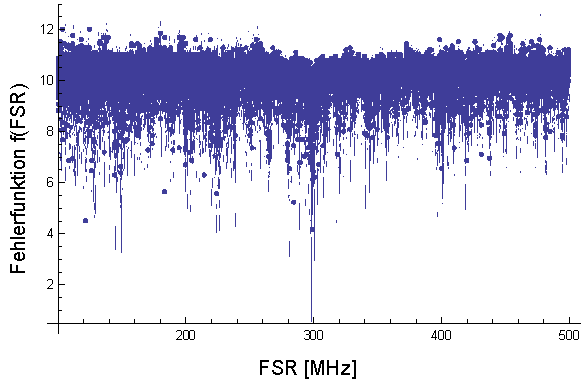
\includegraphics[width=(\textwidth-0.6cm)/2]{plt/nonius_FSR_messung_a}
		}
 	\subfloat[]{
		\label{subfig:nonius_FSR_messung_b}
		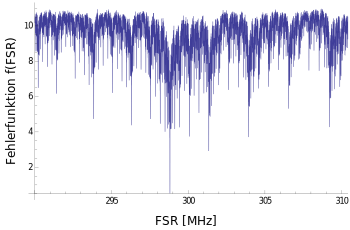
\includegraphics[width=(\textwidth-0.6cm)/2]{plt/nonius_FSR_messung_b}
		}\\
	 \subfloat[]{
		\label{subfig:nonius_FSR_messung_c}
		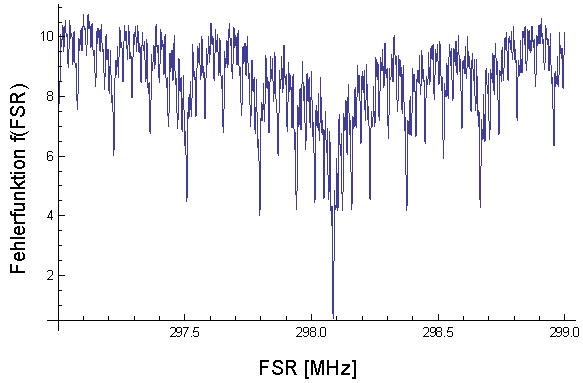
\includegraphics[width=(\textwidth-0.6cm)/2]{plt/nonius_FSR_messung_c}
		}
	\subfloat[]{
		\label{subfig:nonius_FSR_messung_d}
		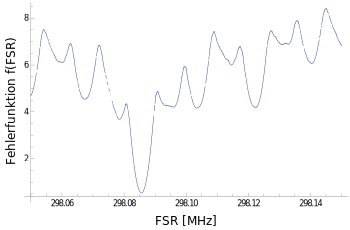
\includegraphics[width=(\textwidth-0.6cm)/2]{plt/nonius_FSR_messung_d}
		}
	}}
	\caption[FSR-Bestimmung]{Plots der Fehlerfunktionen. Von (a) nach (d) wurde der
	Ausschnitt des interessanten Minimums vergrößert. Die Stelle des Minimums ist
	der wahrscheinlichste FSR des FPIs.}
	\label{fig:nonius_FSR_messung}
\end{figure}

\subsection{Finesse}\label{subsec:finesse}
Im Gegensatz zum FSR ist die Finesse ein weniger
kritischer Parameter, sollte dennoch groß genug sein, damit die Spitze der
Transmissionsfringes mit der FOL-Technik präzise detektiert werden
kann. Wie in Abschn. \ref{subsec:fabry-perot-interferometer} erklärt, ist
die Finesse abhängig von der Wellenlänge des Laserlichts. Deshalb wurde für jeden
Wellenlängenbereich der in diesem System verwendeten Laser die Finesse
gemessen. Dazu wurde jeweils mithilfe eines Oszilloskops das Fringepattern bei
ansteigenden Rampe aufgenommen und daran eine Airy-Funktion
\begin{equation}\label{eq:finesse_messung_01}
	U(t,\kappa,a,b,c) = b\cdot\frac{1}{1+\kappa \sin^2{(at)}}+c
\end{equation}
angepasst, wobei $U$ die verstärkte Spannung an der Photodiode, $t$ die Zeit,
$\kappa$ das Maß für die Finesse und $a$, $b$, $c$ Normierungsgrößen sind.
Abbildung \ref{fig:finesse_messung} zeigt die Plots inklusive Fits der
Fringepattern von \textit{DL-Pro} mit $772\,$nm (a), He:Ne-Laser mit $633\,$nm (b), und dem
blauen Diodenlaser mit $405\,$nm (c).
\begin{figure}[h]
 	\centering
 	\footnotesize
 	\fbox{\parbox{\dimexpr \linewidth - 2\fboxrule - 2\fboxsep}{
 	\subfloat[]{
		\label{subfig:finesse_messung_a}
		% GNUPLOT: LaTeX picture with Postscript
\begingroup
  \makeatletter
  \providecommand\color[2][]{%
    \GenericError{(gnuplot) \space\space\space\@spaces}{%
      Package color not loaded in conjunction with
      terminal option `colourtext'%
    }{See the gnuplot documentation for explanation.%
    }{Either use 'blacktext' in gnuplot or load the package
      color.sty in LaTeX.}%
    \renewcommand\color[2][]{}%
  }%
  \providecommand\includegraphics[2][]{%
    \GenericError{(gnuplot) \space\space\space\@spaces}{%
      Package graphicx or graphics not loaded%
    }{See the gnuplot documentation for explanation.%
    }{The gnuplot epslatex terminal needs graphicx.sty or graphics.sty.}%
    \renewcommand\includegraphics[2][]{}%
  }%
  \providecommand\rotatebox[2]{#2}%
  \@ifundefined{ifGPcolor}{%
    \newif\ifGPcolor
    \GPcolortrue
  }{}%
  \@ifundefined{ifGPblacktext}{%
    \newif\ifGPblacktext
    \GPblacktexttrue
  }{}%
  % define a \g@addto@macro without @ in the name:
  \let\gplgaddtomacro\g@addto@macro
  % define empty templates for all commands taking text:
  \gdef\gplbacktext{}%
  \gdef\gplfronttext{}%
  \makeatother
  \ifGPblacktext
    % no textcolor at all
    \def\colorrgb#1{}%
    \def\colorgray#1{}%
  \else
    % gray or color?
    \ifGPcolor
      \def\colorrgb#1{\color[rgb]{#1}}%
      \def\colorgray#1{\color[gray]{#1}}%
      \expandafter\def\csname LTw\endcsname{\color{white}}%
      \expandafter\def\csname LTb\endcsname{\color{black}}%
      \expandafter\def\csname LTa\endcsname{\color{black}}%
      \expandafter\def\csname LT0\endcsname{\color[rgb]{1,0,0}}%
      \expandafter\def\csname LT1\endcsname{\color[rgb]{0,1,0}}%
      \expandafter\def\csname LT2\endcsname{\color[rgb]{0,0,1}}%
      \expandafter\def\csname LT3\endcsname{\color[rgb]{1,0,1}}%
      \expandafter\def\csname LT4\endcsname{\color[rgb]{0,1,1}}%
      \expandafter\def\csname LT5\endcsname{\color[rgb]{1,1,0}}%
      \expandafter\def\csname LT6\endcsname{\color[rgb]{0,0,0}}%
      \expandafter\def\csname LT7\endcsname{\color[rgb]{1,0.3,0}}%
      \expandafter\def\csname LT8\endcsname{\color[rgb]{0.5,0.5,0.5}}%
    \else
      % gray
      \def\colorrgb#1{\color{black}}%
      \def\colorgray#1{\color[gray]{#1}}%
      \expandafter\def\csname LTw\endcsname{\color{white}}%
      \expandafter\def\csname LTb\endcsname{\color{black}}%
      \expandafter\def\csname LTa\endcsname{\color{black}}%
      \expandafter\def\csname LT0\endcsname{\color{black}}%
      \expandafter\def\csname LT1\endcsname{\color{black}}%
      \expandafter\def\csname LT2\endcsname{\color{black}}%
      \expandafter\def\csname LT3\endcsname{\color{black}}%
      \expandafter\def\csname LT4\endcsname{\color{black}}%
      \expandafter\def\csname LT5\endcsname{\color{black}}%
      \expandafter\def\csname LT6\endcsname{\color{black}}%
      \expandafter\def\csname LT7\endcsname{\color{black}}%
      \expandafter\def\csname LT8\endcsname{\color{black}}%
    \fi
  \fi
  \setlength{\unitlength}{0.0500bp}%
  \begin{picture}(7936.00,3968.00)%
    \gplgaddtomacro\gplbacktext{%
      \csname LTb\endcsname%
      \put(980,640){\makebox(0,0)[r]{\strut{} 0}}%
      \put(980,983){\makebox(0,0)[r]{\strut{} 0.01}}%
      \put(980,1326){\makebox(0,0)[r]{\strut{} 0.02}}%
      \put(980,1669){\makebox(0,0)[r]{\strut{} 0.03}}%
      \put(980,2012){\makebox(0,0)[r]{\strut{} 0.04}}%
      \put(980,2355){\makebox(0,0)[r]{\strut{} 0.05}}%
      \put(980,2698){\makebox(0,0)[r]{\strut{} 0.06}}%
      \put(980,3041){\makebox(0,0)[r]{\strut{} 0.07}}%
      \put(980,3384){\makebox(0,0)[r]{\strut{} 0.08}}%
      \put(980,3727){\makebox(0,0)[r]{\strut{} 0.09}}%
      \put(1100,440){\makebox(0,0){\strut{}-6}}%
      \put(1909,440){\makebox(0,0){\strut{}-5}}%
      \put(2719,440){\makebox(0,0){\strut{}-4}}%
      \put(3528,440){\makebox(0,0){\strut{}-3}}%
      \put(4338,440){\makebox(0,0){\strut{}-2}}%
      \put(5147,440){\makebox(0,0){\strut{}-1}}%
      \put(5956,440){\makebox(0,0){\strut{} 0}}%
      \put(6766,440){\makebox(0,0){\strut{} 1}}%
      \put(7575,440){\makebox(0,0){\strut{} 2}}%
      \put(160,2183){\rotatebox{-270}{\makebox(0,0){\strut{}Amplitude U [V]}}}%
      \put(4337,140){\makebox(0,0){\strut{}Zeit t [ms]}}%
      \put(2719,2894){\makebox(0,0)[l]{\strut{}$\kappa = 992\pm14$}}%
      \put(2719,2677){\makebox(0,0)[l]{\strut{}$a = (562.020\pm0.044)\,$s$^{-1}$}}%
      \put(2719,2461){\makebox(0,0)[l]{\strut{}$b = (0.05961\pm0.00028)\,$V}}%
      \put(2719,2245){\makebox(0,0)[l]{\strut{}$c = (0.010994\pm0.000029)\,$V}}%
    }%
    \gplgaddtomacro\gplfronttext{%
      \csname LTb\endcsname%
      \put(6672,3564){\makebox(0,0)[r]{\strut{}Fringepattern}}%
      \csname LTb\endcsname%
      \put(6672,3364){\makebox(0,0)[r]{\strut{}Fit}}%
    }%
    \gplbacktext
    \put(0,0){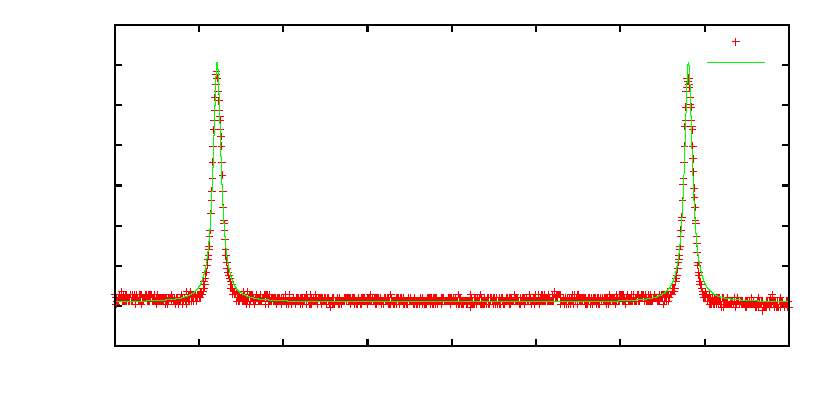
\includegraphics{finesse_messung_a}}%
    \gplfronttext
  \end{picture}%
\endgroup

		}
 	\subfloat[]{
		\label{subfig:finesse_messung_b}
		% GNUPLOT: LaTeX picture with Postscript
\begingroup
  \makeatletter
  \providecommand\color[2][]{%
    \GenericError{(gnuplot) \space\space\space\@spaces}{%
      Package color not loaded in conjunction with
      terminal option `colourtext'%
    }{See the gnuplot documentation for explanation.%
    }{Either use 'blacktext' in gnuplot or load the package
      color.sty in LaTeX.}%
    \renewcommand\color[2][]{}%
  }%
  \providecommand\includegraphics[2][]{%
    \GenericError{(gnuplot) \space\space\space\@spaces}{%
      Package graphicx or graphics not loaded%
    }{See the gnuplot documentation for explanation.%
    }{The gnuplot epslatex terminal needs graphicx.sty or graphics.sty.}%
    \renewcommand\includegraphics[2][]{}%
  }%
  \providecommand\rotatebox[2]{#2}%
  \@ifundefined{ifGPcolor}{%
    \newif\ifGPcolor
    \GPcolortrue
  }{}%
  \@ifundefined{ifGPblacktext}{%
    \newif\ifGPblacktext
    \GPblacktexttrue
  }{}%
  % define a \g@addto@macro without @ in the name:
  \let\gplgaddtomacro\g@addto@macro
  % define empty templates for all commands taking text:
  \gdef\gplbacktext{}%
  \gdef\gplfronttext{}%
  \makeatother
  \ifGPblacktext
    % no textcolor at all
    \def\colorrgb#1{}%
    \def\colorgray#1{}%
  \else
    % gray or color?
    \ifGPcolor
      \def\colorrgb#1{\color[rgb]{#1}}%
      \def\colorgray#1{\color[gray]{#1}}%
      \expandafter\def\csname LTw\endcsname{\color{white}}%
      \expandafter\def\csname LTb\endcsname{\color{black}}%
      \expandafter\def\csname LTa\endcsname{\color{black}}%
      \expandafter\def\csname LT0\endcsname{\color[rgb]{1,0,0}}%
      \expandafter\def\csname LT1\endcsname{\color[rgb]{0,1,0}}%
      \expandafter\def\csname LT2\endcsname{\color[rgb]{0,0,1}}%
      \expandafter\def\csname LT3\endcsname{\color[rgb]{1,0,1}}%
      \expandafter\def\csname LT4\endcsname{\color[rgb]{0,1,1}}%
      \expandafter\def\csname LT5\endcsname{\color[rgb]{1,1,0}}%
      \expandafter\def\csname LT6\endcsname{\color[rgb]{0,0,0}}%
      \expandafter\def\csname LT7\endcsname{\color[rgb]{1,0.3,0}}%
      \expandafter\def\csname LT8\endcsname{\color[rgb]{0.5,0.5,0.5}}%
    \else
      % gray
      \def\colorrgb#1{\color{black}}%
      \def\colorgray#1{\color[gray]{#1}}%
      \expandafter\def\csname LTw\endcsname{\color{white}}%
      \expandafter\def\csname LTb\endcsname{\color{black}}%
      \expandafter\def\csname LTa\endcsname{\color{black}}%
      \expandafter\def\csname LT0\endcsname{\color{black}}%
      \expandafter\def\csname LT1\endcsname{\color{black}}%
      \expandafter\def\csname LT2\endcsname{\color{black}}%
      \expandafter\def\csname LT3\endcsname{\color{black}}%
      \expandafter\def\csname LT4\endcsname{\color{black}}%
      \expandafter\def\csname LT5\endcsname{\color{black}}%
      \expandafter\def\csname LT6\endcsname{\color{black}}%
      \expandafter\def\csname LT7\endcsname{\color{black}}%
      \expandafter\def\csname LT8\endcsname{\color{black}}%
    \fi
  \fi
  \setlength{\unitlength}{0.0500bp}%
  \begin{picture}(7936.00,3968.00)%
    \gplgaddtomacro\gplbacktext{%
      \csname LTb\endcsname%
      \put(860,640){\makebox(0,0)[r]{\strut{}-0.1}}%
      \put(860,1026){\makebox(0,0)[r]{\strut{} 0}}%
      \put(860,1412){\makebox(0,0)[r]{\strut{} 0.1}}%
      \put(860,1798){\makebox(0,0)[r]{\strut{} 0.2}}%
      \put(860,2184){\makebox(0,0)[r]{\strut{} 0.3}}%
      \put(860,2569){\makebox(0,0)[r]{\strut{} 0.4}}%
      \put(860,2955){\makebox(0,0)[r]{\strut{} 0.5}}%
      \put(860,3341){\makebox(0,0)[r]{\strut{} 0.6}}%
      \put(860,3727){\makebox(0,0)[r]{\strut{} 0.7}}%
      \put(980,440){\makebox(0,0){\strut{}-2}}%
      \put(1922,440){\makebox(0,0){\strut{}-1}}%
      \put(2864,440){\makebox(0,0){\strut{} 0}}%
      \put(3806,440){\makebox(0,0){\strut{} 1}}%
      \put(4749,440){\makebox(0,0){\strut{} 2}}%
      \put(5691,440){\makebox(0,0){\strut{} 3}}%
      \put(6633,440){\makebox(0,0){\strut{} 4}}%
      \put(7575,440){\makebox(0,0){\strut{} 5}}%
      \put(160,2183){\rotatebox{-270}{\makebox(0,0){\strut{}Amplitude U [V]}}}%
      \put(4277,140){\makebox(0,0){\strut{}Zeit t [ms]}}%
      \put(2629,2894){\makebox(0,0)[l]{\strut{}$\kappa = 522.6\pm6.9$}}%
      \put(2629,2677){\makebox(0,0)[l]{\strut{}$a = (686.405\pm0.068)\,$s$^{-1}$}}%
      \put(2629,2461){\makebox(0,0)[l]{\strut{}$b = (0.5879\pm0.0026)\,$V}}%
      \put(2629,2245){\makebox(0,0)[l]{\strut{}$c = (-0.02542\pm0.00035)\,$V}}%
    }%
    \gplgaddtomacro\gplfronttext{%
      \csname LTb\endcsname%
      \put(6672,3564){\makebox(0,0)[r]{\strut{}Fringepattern}}%
      \csname LTb\endcsname%
      \put(6672,3364){\makebox(0,0)[r]{\strut{}Fit}}%
    }%
    \gplbacktext
    \put(0,0){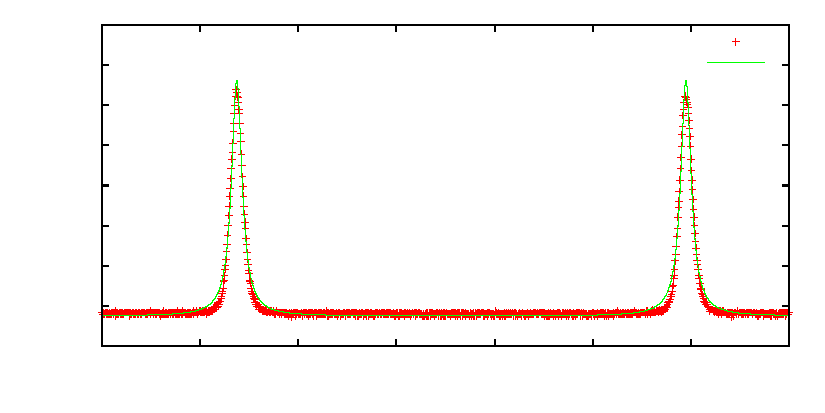
\includegraphics{finesse_messung_b}}%
    \gplfronttext
  \end{picture}%
\endgroup

		}\\
	\centering
	\subfloat[]{
		\label{subfig:finesse_messung_c}
		% GNUPLOT: LaTeX picture with Postscript
\begingroup
  \makeatletter
  \providecommand\color[2][]{%
    \GenericError{(gnuplot) \space\space\space\@spaces}{%
      Package color not loaded in conjunction with
      terminal option `colourtext'%
    }{See the gnuplot documentation for explanation.%
    }{Either use 'blacktext' in gnuplot or load the package
      color.sty in LaTeX.}%
    \renewcommand\color[2][]{}%
  }%
  \providecommand\includegraphics[2][]{%
    \GenericError{(gnuplot) \space\space\space\@spaces}{%
      Package graphicx or graphics not loaded%
    }{See the gnuplot documentation for explanation.%
    }{The gnuplot epslatex terminal needs graphicx.sty or graphics.sty.}%
    \renewcommand\includegraphics[2][]{}%
  }%
  \providecommand\rotatebox[2]{#2}%
  \@ifundefined{ifGPcolor}{%
    \newif\ifGPcolor
    \GPcolortrue
  }{}%
  \@ifundefined{ifGPblacktext}{%
    \newif\ifGPblacktext
    \GPblacktexttrue
  }{}%
  % define a \g@addto@macro without @ in the name:
  \let\gplgaddtomacro\g@addto@macro
  % define empty templates for all commands taking text:
  \gdef\gplbacktext{}%
  \gdef\gplfronttext{}%
  \makeatother
  \ifGPblacktext
    % no textcolor at all
    \def\colorrgb#1{}%
    \def\colorgray#1{}%
  \else
    % gray or color?
    \ifGPcolor
      \def\colorrgb#1{\color[rgb]{#1}}%
      \def\colorgray#1{\color[gray]{#1}}%
      \expandafter\def\csname LTw\endcsname{\color{white}}%
      \expandafter\def\csname LTb\endcsname{\color{black}}%
      \expandafter\def\csname LTa\endcsname{\color{black}}%
      \expandafter\def\csname LT0\endcsname{\color[rgb]{1,0,0}}%
      \expandafter\def\csname LT1\endcsname{\color[rgb]{0,1,0}}%
      \expandafter\def\csname LT2\endcsname{\color[rgb]{0,0,1}}%
      \expandafter\def\csname LT3\endcsname{\color[rgb]{1,0,1}}%
      \expandafter\def\csname LT4\endcsname{\color[rgb]{0,1,1}}%
      \expandafter\def\csname LT5\endcsname{\color[rgb]{1,1,0}}%
      \expandafter\def\csname LT6\endcsname{\color[rgb]{0,0,0}}%
      \expandafter\def\csname LT7\endcsname{\color[rgb]{1,0.3,0}}%
      \expandafter\def\csname LT8\endcsname{\color[rgb]{0.5,0.5,0.5}}%
    \else
      % gray
      \def\colorrgb#1{\color{black}}%
      \def\colorgray#1{\color[gray]{#1}}%
      \expandafter\def\csname LTw\endcsname{\color{white}}%
      \expandafter\def\csname LTb\endcsname{\color{black}}%
      \expandafter\def\csname LTa\endcsname{\color{black}}%
      \expandafter\def\csname LT0\endcsname{\color{black}}%
      \expandafter\def\csname LT1\endcsname{\color{black}}%
      \expandafter\def\csname LT2\endcsname{\color{black}}%
      \expandafter\def\csname LT3\endcsname{\color{black}}%
      \expandafter\def\csname LT4\endcsname{\color{black}}%
      \expandafter\def\csname LT5\endcsname{\color{black}}%
      \expandafter\def\csname LT6\endcsname{\color{black}}%
      \expandafter\def\csname LT7\endcsname{\color{black}}%
      \expandafter\def\csname LT8\endcsname{\color{black}}%
    \fi
  \fi
  \setlength{\unitlength}{0.0500bp}%
  \begin{picture}(7936.00,3968.00)%
    \gplgaddtomacro\gplbacktext{%
      \csname LTb\endcsname%
      \put(860,640){\makebox(0,0)[r]{\strut{} 1}}%
      \put(860,983){\makebox(0,0)[r]{\strut{} 1.5}}%
      \put(860,1326){\makebox(0,0)[r]{\strut{} 2}}%
      \put(860,1669){\makebox(0,0)[r]{\strut{} 2.5}}%
      \put(860,2012){\makebox(0,0)[r]{\strut{} 3}}%
      \put(860,2355){\makebox(0,0)[r]{\strut{} 3.5}}%
      \put(860,2698){\makebox(0,0)[r]{\strut{} 4}}%
      \put(860,3041){\makebox(0,0)[r]{\strut{} 4.5}}%
      \put(860,3384){\makebox(0,0)[r]{\strut{} 5}}%
      \put(860,3727){\makebox(0,0)[r]{\strut{} 5.5}}%
      \put(1451,440){\makebox(0,0){\strut{}-3}}%
      \put(2393,440){\makebox(0,0){\strut{}-2}}%
      \put(3335,440){\makebox(0,0){\strut{}-1}}%
      \put(4277,440){\makebox(0,0){\strut{} 0}}%
      \put(5220,440){\makebox(0,0){\strut{} 1}}%
      \put(6162,440){\makebox(0,0){\strut{} 2}}%
      \put(7104,440){\makebox(0,0){\strut{} 3}}%
      \put(160,2183){\rotatebox{-270}{\makebox(0,0){\strut{}Amplitude U [V]}}}%
      \put(4277,140){\makebox(0,0){\strut{}Zeit t [ms]}}%
      \put(2629,1597){\makebox(0,0)[l]{\strut{}$\kappa = 1.515\pm0.026$}}%
      \put(2629,1381){\makebox(0,0)[l]{\strut{}$a = (1065.75\pm0.51)\,$s$^{-1}$}}%
      \put(2629,1165){\makebox(0,0)[l]{\strut{}$b = (2.917\pm0.020)\,$V}}%
      \put(2629,949){\makebox(0,0)[l]{\strut{}$c = (1.690\pm0.022)\,$V}}%
    }%
    \gplgaddtomacro\gplfronttext{%
      \csname LTb\endcsname%
      \put(6672,3564){\makebox(0,0)[r]{\strut{}Fringepattern}}%
      \csname LTb\endcsname%
      \put(6672,3364){\makebox(0,0)[r]{\strut{}Fit}}%
    }%
    \gplbacktext
    \put(0,0){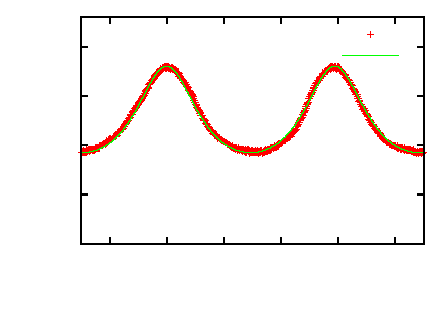
\includegraphics{finesse_messung_c}}%
    \gplfronttext
  \end{picture}%
\endgroup

		}
	}}
	\caption[Finesse des FPIs]{Plots des Fringepattern für $772\,$nm (a), $633\,$nm
	(b) und $405\,$nm (c).}
	\label{fig:finesse_messung}
\end{figure}
Aus den Fits lassen sich die jeweiligen Reflektivitäten der Spiegel für die
Wellenlängen über
\begin{equation}\label{eq:finesse_messung_02}
	\begin{split}
		\kappa&=\frac{4R}{(1-R)^2}\\
		&\Rightarrow\\
		R&=\frac{2+\kappa\pm2\sqrt{1+\kappa}}{\kappa}
	\end{split}	
\end{equation}
berechnen, wobei nur die Lösung mit dem negativen Vorzeichen physikalisch ist.
Tabelle \ref{tab:finesse} führt alle Reflektivitäten und Finessen (nach
Gl. \eqref{eq:FPI_finesse}) auf. Wie schon in Abschn. \ref{sec:lasersystem}
erwähnt, hat das FPI im blauen Bereich eine sehr schlechte Finesse, mit der allerdings immernoch hinreichend präzise detektiert werden kann. Im infraroten
Bereich hat das FPI offensichtlich die höchste Finesse.
\begin{table}[h]
	%Summe der Breiten muss 0.91 mal \textwidth sein.
	\begin{tabular}{ccc}
		\toprule
		\multicolumn{1}{C{0.30\textwidth}}{Wellenlänge [nm]} &
		\multicolumn{1}{C{0.31\textwidth}}{Spiegelreflektivität} &
		\multicolumn{1}{C{0.30\textwidth}}{Finesse}\\
		\midrule[1px]
		\hline
		%%%%%%%%%%%%%%%%%%%%%%%%%%%%%%%%%%%%%%%%%%%%%%%%%%%%%%%%%%%%%%%%%%%%%%
%%                                                                  %%
%%  This is a LaTeX2e table fragment exported from Gnumeric.        %%
%%                                                                  %%
%%%%%%%%%%%%%%%%%%%%%%%%%%%%%%%%%%%%%%%%%%%%%%%%%%%%%%%%%%%%%%%%%%%%%%
%Wellenlänge [nm]	&Spiegelreflektivität	&Finesse\\
772	&0,938	&49,47\\
633	&0,916	&35,79\\
405	&0,227	&1,936\\

		\bottomrule[1px]
	\end{tabular}
	\caption[FPI Finesse]{Messwerte für die Reflektivität der
	Spiegel und die Finesse des FPIs in Abhängigkeit von der Wellenlänge.}
	\label{tab:finesse}
\end{table}

\section{Stabilität der Laser}\label{sec:stabilitaet_der_laser}
Um die Lang- und Kurzzeitstabilität der Laser zu untersuchen wurden zwei
verschiedene Methoden angewandt. Zum einen wurde sowohl vom alten als auch vom
neuen Lasersystem das Frequenzverhalten mithilfe der neu entwickelte Software
aufgezeichnet. Zum anderen wurden Schwebungsfrequenzmessungen zweier Laser mit
nahezu gleicher Frequenz durchgeführt, die Relativfrequenzdaten beider Laser
liefern. Die Ergebnisse dieser beiden Methoden sollen in diesem Abschnitt
vorgestellt werden. Dabei wurde das alte System ausschließlich mit der alten und
das neue ausschließlich mit der im Ramen dieser Arbeit entwickelten
neuen Regelung stabilsiliert.

\subsection{Stabilitätsmessung mit neuer
Software}\label{sec:stabilitaetsmessungen_software} Das Frequenzverhalten
aller drei Laser des neuen Systems wurde mit der neu entwickelten Software über zwei Stunden hinweg analysiert, wobei die
Laser jeweils in den Modi freilaufend, \textit{iScan}-stabilisiert und
\textit{iScan}+FOL-stabilisiert gemessen wurden. Zusätzlich wurde repräsentativ
für das alte System das Frequenzverhalten des Lasers für den zweiten
Anregungsschritt mit der neuen Software aufgezeichnet, während dieser
mit der alten FOL-Technik stabilisiert wurde.

\subsubsection{Laserstabilität im neuen
System}\label{subsubsec:stabilitaetsmessungen_software_neues_system}
\begin{figure}[h]
 	\centering
 	\footnotesize
	% GNUPLOT: LaTeX picture with Postscript
\begingroup
  \makeatletter
  \providecommand\color[2][]{%
    \GenericError{(gnuplot) \space\space\space\@spaces}{%
      Package color not loaded in conjunction with
      terminal option `colourtext'%
    }{See the gnuplot documentation for explanation.%
    }{Either use 'blacktext' in gnuplot or load the package
      color.sty in LaTeX.}%
    \renewcommand\color[2][]{}%
  }%
  \providecommand\includegraphics[2][]{%
    \GenericError{(gnuplot) \space\space\space\@spaces}{%
      Package graphicx or graphics not loaded%
    }{See the gnuplot documentation for explanation.%
    }{The gnuplot epslatex terminal needs graphicx.sty or graphics.sty.}%
    \renewcommand\includegraphics[2][]{}%
  }%
  \providecommand\rotatebox[2]{#2}%
  \@ifundefined{ifGPcolor}{%
    \newif\ifGPcolor
    \GPcolortrue
  }{}%
  \@ifundefined{ifGPblacktext}{%
    \newif\ifGPblacktext
    \GPblacktexttrue
  }{}%
  % define a \g@addto@macro without @ in the name:
  \let\gplgaddtomacro\g@addto@macro
  % define empty templates for all commands taking text:
  \gdef\gplbacktext{}%
  \gdef\gplfronttext{}%
  \makeatother
  \ifGPblacktext
    % no textcolor at all
    \def\colorrgb#1{}%
    \def\colorgray#1{}%
  \else
    % gray or color?
    \ifGPcolor
      \def\colorrgb#1{\color[rgb]{#1}}%
      \def\colorgray#1{\color[gray]{#1}}%
      \expandafter\def\csname LTw\endcsname{\color{white}}%
      \expandafter\def\csname LTb\endcsname{\color{black}}%
      \expandafter\def\csname LTa\endcsname{\color{black}}%
      \expandafter\def\csname LT0\endcsname{\color[rgb]{1,0,0}}%
      \expandafter\def\csname LT1\endcsname{\color[rgb]{0,1,0}}%
      \expandafter\def\csname LT2\endcsname{\color[rgb]{0,0,1}}%
      \expandafter\def\csname LT3\endcsname{\color[rgb]{1,0,1}}%
      \expandafter\def\csname LT4\endcsname{\color[rgb]{0,1,1}}%
      \expandafter\def\csname LT5\endcsname{\color[rgb]{1,1,0}}%
      \expandafter\def\csname LT6\endcsname{\color[rgb]{0,0,0}}%
      \expandafter\def\csname LT7\endcsname{\color[rgb]{1,0.3,0}}%
      \expandafter\def\csname LT8\endcsname{\color[rgb]{0.5,0.5,0.5}}%
    \else
      % gray
      \def\colorrgb#1{\color{black}}%
      \def\colorgray#1{\color[gray]{#1}}%
      \expandafter\def\csname LTw\endcsname{\color{white}}%
      \expandafter\def\csname LTb\endcsname{\color{black}}%
      \expandafter\def\csname LTa\endcsname{\color{black}}%
      \expandafter\def\csname LT0\endcsname{\color{black}}%
      \expandafter\def\csname LT1\endcsname{\color{black}}%
      \expandafter\def\csname LT2\endcsname{\color{black}}%
      \expandafter\def\csname LT3\endcsname{\color{black}}%
      \expandafter\def\csname LT4\endcsname{\color{black}}%
      \expandafter\def\csname LT5\endcsname{\color{black}}%
      \expandafter\def\csname LT6\endcsname{\color{black}}%
      \expandafter\def\csname LT7\endcsname{\color{black}}%
      \expandafter\def\csname LT8\endcsname{\color{black}}%
    \fi
  \fi
  \setlength{\unitlength}{0.0500bp}%
  \begin{picture}(8502.00,6802.00)%
    \gplgaddtomacro\gplbacktext{%
      \csname LTb\endcsname%
      \put(1080,3401){\makebox(0,0)[r]{\strut{}-60}}%
      \put(1080,3796){\makebox(0,0)[r]{\strut{}-50}}%
      \put(1080,4191){\makebox(0,0)[r]{\strut{}-40}}%
      \put(1080,4586){\makebox(0,0)[r]{\strut{}-30}}%
      \put(1080,4981){\makebox(0,0)[r]{\strut{}-20}}%
      \put(1080,5376){\makebox(0,0)[r]{\strut{}-10}}%
      \put(1080,5771){\makebox(0,0)[r]{\strut{} 0}}%
      \put(1080,6166){\makebox(0,0)[r]{\strut{} 10}}%
      \put(1080,6561){\makebox(0,0)[r]{\strut{} 20}}%
      \put(1200,3201){\makebox(0,0){\strut{}}}%
      \put(2357,3201){\makebox(0,0){\strut{}}}%
      \put(3514,3201){\makebox(0,0){\strut{}}}%
      \put(4671,3201){\makebox(0,0){\strut{}}}%
      \put(5827,3201){\makebox(0,0){\strut{}}}%
      \put(6984,3201){\makebox(0,0){\strut{}}}%
      \put(8141,3201){\makebox(0,0){\strut{}}}%
      \put(500,4981){\rotatebox{-270}{\makebox(0,0){\strut{}relative Frequenz [MHz]}}}%
    }%
    \gplgaddtomacro\gplfronttext{%
      \csname LTb\endcsname%
      \put(5040,3964){\makebox(0,0)[r]{\strut{}freilaufend}}%
      \csname LTb\endcsname%
      \put(5040,3764){\makebox(0,0)[r]{\strut{}\textit{iScan}-stabilisiert}}%
      \csname LTb\endcsname%
      \put(5040,3564){\makebox(0,0)[r]{\strut{}\textit{iScan}+FOL-stabilisiert}}%
    }%
    \gplgaddtomacro\gplbacktext{%
      \csname LTb\endcsname%
      \put(1080,2585){\makebox(0,0)[r]{\strut{} 0.5}}%
      \put(1080,2791){\makebox(0,0)[r]{\strut{} 1}}%
      \put(1080,2996){\makebox(0,0)[r]{\strut{} 1.5}}%
      \put(1200,2180){\makebox(0,0){\strut{}}}%
      \put(2357,2180){\makebox(0,0){\strut{}}}%
      \put(3514,2180){\makebox(0,0){\strut{}}}%
      \put(4671,2180){\makebox(0,0){\strut{}}}%
      \put(5827,2180){\makebox(0,0){\strut{}}}%
      \put(6984,2180){\makebox(0,0){\strut{}}}%
      \put(8141,2180){\makebox(0,0){\strut{}}}%
    }%
    \gplgaddtomacro\gplfronttext{%
    }%
    \gplgaddtomacro\gplbacktext{%
      \csname LTb\endcsname%
      \put(1080,1615){\makebox(0,0)[r]{\strut{} 0.5}}%
      \put(1080,1870){\makebox(0,0)[r]{\strut{} 1}}%
      \put(1080,2125){\makebox(0,0)[r]{\strut{} 1.5}}%
      \put(1200,1160){\makebox(0,0){\strut{}}}%
      \put(2357,1160){\makebox(0,0){\strut{}}}%
      \put(3514,1160){\makebox(0,0){\strut{}}}%
      \put(4671,1160){\makebox(0,0){\strut{}}}%
      \put(5827,1160){\makebox(0,0){\strut{}}}%
      \put(6984,1160){\makebox(0,0){\strut{}}}%
      \put(8141,1160){\makebox(0,0){\strut{}}}%
      \put(500,1870){\rotatebox{-270}{\makebox(0,0){\strut{}Jitter [MHz]}}}%
    }%
    \gplgaddtomacro\gplfronttext{%
    }%
    \gplgaddtomacro\gplbacktext{%
      \csname LTb\endcsname%
      \put(1080,790){\makebox(0,0)[r]{\strut{} 0.5}}%
      \put(1080,980){\makebox(0,0)[r]{\strut{} 1}}%
      \put(1080,1170){\makebox(0,0)[r]{\strut{} 1.5}}%
      \put(1200,400){\makebox(0,0){\strut{}0}}%
      \put(2357,400){\makebox(0,0){\strut{}20}}%
      \put(3514,400){\makebox(0,0){\strut{}40}}%
      \put(4671,400){\makebox(0,0){\strut{}60}}%
      \put(5827,400){\makebox(0,0){\strut{}80}}%
      \put(6984,400){\makebox(0,0){\strut{}100}}%
      \put(8141,400){\makebox(0,0){\strut{}120}}%
      \put(4670,100){\makebox(0,0){\strut{}Zeit [min]}}%
    }%
    \gplgaddtomacro\gplfronttext{%
    }%
    \gplbacktext
    \put(0,0){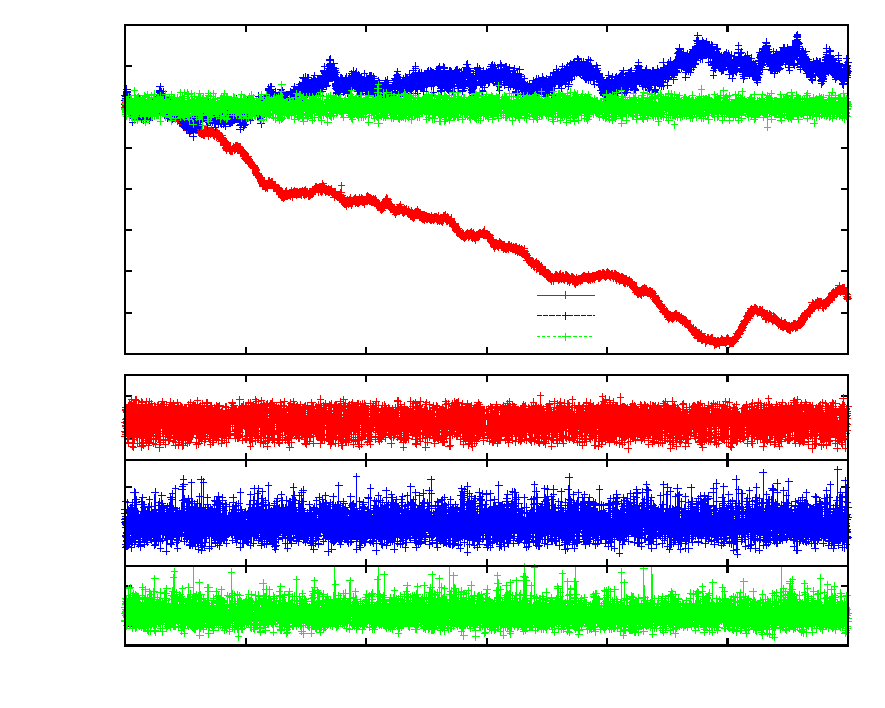
\includegraphics{laserstabilitaet_b_alles}}%
    \gplfronttext
  \end{picture}%
\endgroup

	\caption[Laserfrequenzverhalten \textit{DL-Pro}]{Laserfrequenzverhalten des
	\textit{DL-Pro} im freilaufenden (rot), \textit{iScan}-stabiliserten (blau) und
	\textit{iScan}+FOL-stabiliserten Modus (grün). Darunter ist jeweils
	entsprechend farblich kodiert der Jitter aufgetragen. Separate,
	hochaufgelöstere Plots für alle Laser finden sich in Anh.
	\ref{anh:sec:laserstabilitaet}.}
	\label{fig:laserstabilitaet_b_alles}
\end{figure}
Abbildung \ref{fig:laserstabilitaet_b_alles} zeigt den relativen
Frequenzverlauf des \textit{DL-Pro} im freilaufenden (rot),
\textit{iScan}-stabilisierten (blau) und \textit{iScan}+FOL-stabilisierten Modus
(grün). Die Plots für die anderen beiden Laser befinden sich in Anh.
\ref{anh:sec:laserstabilitaet}. Sind die Laser nicht aktiv stabilisiert, driften
sie deutlich in der Frequenz. Der \textit{DL-Pro} driftet in zwei Stunden bis zu $60\,$MHz, wohingehen der
\textit{TA-Pro} nur eine maximale Drift von $20\,$MHz aufweist. Dieser
Unterschied beinhaltet allerdings keine Systematik, da auch beim \textit{TA-Pro}
schon größere Drifts beobachtet wurden. Sehr viel größere Frequenzfluktuationen (bis $700\,$MHz)
weist der blaue Laser auf, was auf die wesentlich instabilere Mechanik
zurückzuführen ist. Größtenteils sind die Drifts vermutlich mit der Temperatur
korreliert, was hier allerdings nicht nachgeprüft wurde. Eine weitere Ursache
ist der Piezoaktuator des Gitters, der nach Ändern der Spannung noch lange in
die gleiche Richtung nachdriftet. Der Jitter der Laser (Standardabweichung der
Frequenz über die durch den \textit{Arduino} gemittelten Werte) liegt für die
beiden \textit{Toptica}-Lasern bei maximal $1,5\,$MHz. Für den blauen Laser
liegt dieser bei etwa $5\,$MHz.\par
Wie erwartet reduziert sich die Drift bei \textit{iScan}-Stabilisierung auf ca. $20\,$MHz,
verschwindet aber nicht völlig. Für den \textit{TA-Pro} ist die
\textit{iScan}-Stabilisierung kein besonderer Mehrgewinn, was allerdings wie
schon erwähnt nur speziell auf diese Messung zutreffend ist. Der blaue Laser
erfährt einen dramatischen Zugewinn an Stabilität mit einer Reduzierung der
Drift auf ca. $100\,$MHz. Es zeigt sich, dass die \textit{iScans} zwar
eine hinreichend gute Stabilität in kurzen Zeitintervallen gewährleisten, jedoch
auf größeren Zeitskalen statistischen Schwankungen unterworfen sind. Die
wahrscheinlichste Ursache ist die sensible räumliche Abhängigkeit der
Einkopplung in die \textit{iScan heads}, was sich durch den alternativen Ansatz
einer Faserkopplung überprüfen ließe. Dies ist jedoch eine eigenständige,
kommerzielle Option, die aktuell nicht zur Verfügung steht. Eine weitere Ursache
könnte trotz Temperaturkontrolle die fehlende aktive Stabilisierung der internen \textit{iScan}-Optik sein. Der Jitter ändert sich im Vergleich zum freilaufenden Fall nicht merklich,
weist aber ab und zu kleinere Überhöhungen auf, die mit der Regelung der
\textit{iScans} und/oder des FOL zu erklären sind.\par
%TODO: evtl. periodische Schwingung des Jitters erwähnen
Um die Drifts völlig zu eliminieren, muss das FOL hinzugeschaltet werden. Wie
Abb. \ref{fig:laserstabilitaet_b_alles} zeigt, reduziert sich
durch das FOL die Drift auf nahezu $0\,$MHz. Die Fluktuationen um die
Soll-Relativfrequenz (hier $0\,$MHz) ergibt sich nur noch aus dem Jitter der
Laser und der Regelung des FOL zu maximal $\pm12\,$MHz für den blauen und
$\pm4\,$MHz für die beiden roten Laser. Dieses Frequenzrauschen lässt sich ggf.
noch durch Variation der Ober- und Untergrenzen für das FOL verkleinern, kann
aber bei zu eng gewählten Grenzen zu Überreglung und somit zu größeren
Fluktuationen oder sogar dem Auftreten von Schwingungen führen.
\subsubsection{Laserstabilität im alten
System}\label{subsubsec:stabilitaetsmessungen_software_altes_system}
\begin{figure}[h]
 	\centering
 	\footnotesize
	% GNUPLOT: LaTeX picture with Postscript
\begingroup
  \makeatletter
  \providecommand\color[2][]{%
    \GenericError{(gnuplot) \space\space\space\@spaces}{%
      Package color not loaded in conjunction with
      terminal option `colourtext'%
    }{See the gnuplot documentation for explanation.%
    }{Either use 'blacktext' in gnuplot or load the package
      color.sty in LaTeX.}%
    \renewcommand\color[2][]{}%
  }%
  \providecommand\includegraphics[2][]{%
    \GenericError{(gnuplot) \space\space\space\@spaces}{%
      Package graphicx or graphics not loaded%
    }{See the gnuplot documentation for explanation.%
    }{The gnuplot epslatex terminal needs graphicx.sty or graphics.sty.}%
    \renewcommand\includegraphics[2][]{}%
  }%
  \providecommand\rotatebox[2]{#2}%
  \@ifundefined{ifGPcolor}{%
    \newif\ifGPcolor
    \GPcolortrue
  }{}%
  \@ifundefined{ifGPblacktext}{%
    \newif\ifGPblacktext
    \GPblacktexttrue
  }{}%
  % define a \g@addto@macro without @ in the name:
  \let\gplgaddtomacro\g@addto@macro
  % define empty templates for all commands taking text:
  \gdef\gplbacktext{}%
  \gdef\gplfronttext{}%
  \makeatother
  \ifGPblacktext
    % no textcolor at all
    \def\colorrgb#1{}%
    \def\colorgray#1{}%
  \else
    % gray or color?
    \ifGPcolor
      \def\colorrgb#1{\color[rgb]{#1}}%
      \def\colorgray#1{\color[gray]{#1}}%
      \expandafter\def\csname LTw\endcsname{\color{white}}%
      \expandafter\def\csname LTb\endcsname{\color{black}}%
      \expandafter\def\csname LTa\endcsname{\color{black}}%
      \expandafter\def\csname LT0\endcsname{\color[rgb]{1,0,0}}%
      \expandafter\def\csname LT1\endcsname{\color[rgb]{0,1,0}}%
      \expandafter\def\csname LT2\endcsname{\color[rgb]{0,0,1}}%
      \expandafter\def\csname LT3\endcsname{\color[rgb]{1,0,1}}%
      \expandafter\def\csname LT4\endcsname{\color[rgb]{0,1,1}}%
      \expandafter\def\csname LT5\endcsname{\color[rgb]{1,1,0}}%
      \expandafter\def\csname LT6\endcsname{\color[rgb]{0,0,0}}%
      \expandafter\def\csname LT7\endcsname{\color[rgb]{1,0.3,0}}%
      \expandafter\def\csname LT8\endcsname{\color[rgb]{0.5,0.5,0.5}}%
    \else
      % gray
      \def\colorrgb#1{\color{black}}%
      \def\colorgray#1{\color[gray]{#1}}%
      \expandafter\def\csname LTw\endcsname{\color{white}}%
      \expandafter\def\csname LTb\endcsname{\color{black}}%
      \expandafter\def\csname LTa\endcsname{\color{black}}%
      \expandafter\def\csname LT0\endcsname{\color{black}}%
      \expandafter\def\csname LT1\endcsname{\color{black}}%
      \expandafter\def\csname LT2\endcsname{\color{black}}%
      \expandafter\def\csname LT3\endcsname{\color{black}}%
      \expandafter\def\csname LT4\endcsname{\color{black}}%
      \expandafter\def\csname LT5\endcsname{\color{black}}%
      \expandafter\def\csname LT6\endcsname{\color{black}}%
      \expandafter\def\csname LT7\endcsname{\color{black}}%
      \expandafter\def\csname LT8\endcsname{\color{black}}%
    \fi
  \fi
  \setlength{\unitlength}{0.0500bp}%
  \begin{picture}(8502.00,6802.00)%
    \gplgaddtomacro\gplbacktext{%
      \csname LTb\endcsname%
      \put(1080,2380){\makebox(0,0)[r]{\strut{}-100}}%
      \put(1080,2977){\makebox(0,0)[r]{\strut{}-50}}%
      \put(1080,3575){\makebox(0,0)[r]{\strut{} 0}}%
      \put(1080,4172){\makebox(0,0)[r]{\strut{} 50}}%
      \put(1080,4769){\makebox(0,0)[r]{\strut{} 100}}%
      \put(1080,5366){\makebox(0,0)[r]{\strut{} 150}}%
      \put(1080,5964){\makebox(0,0)[r]{\strut{} 200}}%
      \put(1080,6561){\makebox(0,0)[r]{\strut{} 250}}%
      \put(1200,2180){\makebox(0,0){\strut{}}}%
      \put(2357,2180){\makebox(0,0){\strut{}}}%
      \put(3514,2180){\makebox(0,0){\strut{}}}%
      \put(4671,2180){\makebox(0,0){\strut{}}}%
      \put(5827,2180){\makebox(0,0){\strut{}}}%
      \put(6984,2180){\makebox(0,0){\strut{}}}%
      \put(8141,2180){\makebox(0,0){\strut{}}}%
      \put(380,4470){\rotatebox{-270}{\makebox(0,0){\strut{}relative Frequenz [MHz]}}}%
    }%
    \gplgaddtomacro\gplfronttext{%
      \csname LTb\endcsname%
      \put(3240,2743){\makebox(0,0)[r]{\strut{}freilaufend}}%
      \csname LTb\endcsname%
      \put(3240,2543){\makebox(0,0)[r]{\strut{}FOL-stabilisiert}}%
    }%
    \gplgaddtomacro\gplbacktext{%
      \csname LTb\endcsname%
      \put(1080,1565){\makebox(0,0)[r]{\strut{} 5}}%
      \put(1080,1770){\makebox(0,0)[r]{\strut{} 10}}%
      \put(1080,1975){\makebox(0,0)[r]{\strut{} 15}}%
      \put(1200,1160){\makebox(0,0){\strut{}}}%
      \put(2357,1160){\makebox(0,0){\strut{}}}%
      \put(3514,1160){\makebox(0,0){\strut{}}}%
      \put(4671,1160){\makebox(0,0){\strut{}}}%
      \put(5827,1160){\makebox(0,0){\strut{}}}%
      \put(6984,1160){\makebox(0,0){\strut{}}}%
      \put(8141,1160){\makebox(0,0){\strut{}}}%
      \put(500,1470){\rotatebox{-270}{\makebox(0,0){\strut{}Jitter [MHz]}}}%
    }%
    \gplgaddtomacro\gplfronttext{%
    }%
    \gplgaddtomacro\gplbacktext{%
      \csname LTb\endcsname%
      \put(1080,790){\makebox(0,0)[r]{\strut{} 5}}%
      \put(1080,980){\makebox(0,0)[r]{\strut{} 10}}%
      \put(1080,1170){\makebox(0,0)[r]{\strut{} 15}}%
      \put(1200,400){\makebox(0,0){\strut{}0}}%
      \put(2357,400){\makebox(0,0){\strut{}20}}%
      \put(3514,400){\makebox(0,0){\strut{}40}}%
      \put(4671,400){\makebox(0,0){\strut{}60}}%
      \put(5827,400){\makebox(0,0){\strut{}80}}%
      \put(6984,400){\makebox(0,0){\strut{}100}}%
      \put(8141,400){\makebox(0,0){\strut{}120}}%
      \put(4670,100){\makebox(0,0){\strut{}Zeit [min]}}%
    }%
    \gplgaddtomacro\gplfronttext{%
    }%
    \gplbacktext
    \put(0,0){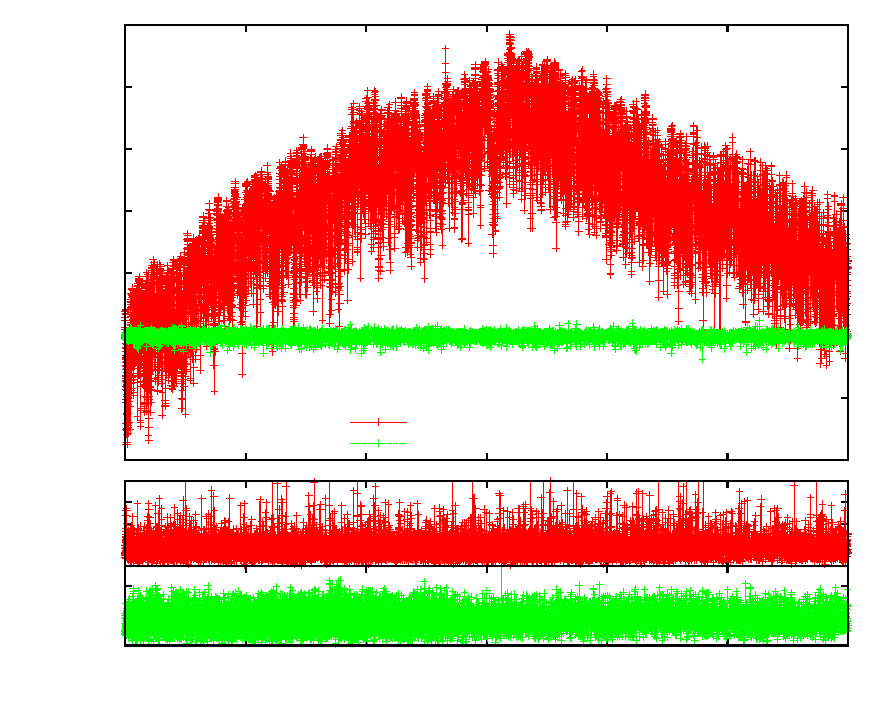
\includegraphics{laserstabilitaet_alt_alles}}%
    \gplfronttext
  \end{picture}%
\endgroup

	\caption[Laserfrequenzverhalten altes System]{Frequenzverhalten des Lasers für
	den zweiten Anregungsschritts im alten System im freilaufenden (rot) und
	FOL-stabiliserten Modus (grün). Unten ist jeweils in des entsprechenden Farben
	der Jitter aufgetragen. Separate, hochaufgelöstere Plots hierfür finden sich in
	Anh. \ref{anh:sec:laserstabilitaet}.}
	\label{fig:laserstabilitaet_alt_alles}
\end{figure}
Abbildung \ref{fig:laserstabilitaet_alt_alles} zeigt die Plots für den
roten Laser des zweiten Anregungsschritts im alten System, dessen Daten auch
über zwei Stunden, aber mit einer höreren Rate\footnote{Die Daten wurden zu
einem Zeitpunkt aufgenommen, an dem die Software bereits in einem performanteren
Stadium war und mit einer höheren Rate Laserdaten verarbeiten konnte. Die Anzahl
der Rampenzyklen zur Zeitenmittlung ist von 10 auf 5 gesunken, was die Rate
der Jitterberechnung von ein Wert pro $170\,$ms auf ein Wert pro $85\,$ms
erhöht.} aufgenommen wurden (rot:
freilaufend; grün:
FOL-stabilisiert).
Separate, hochaufgelöste Plots finden sich im Anh.
\ref{anh:sec:laserstabilitaet}. Im freilaufenden Modus driftet der Laser bis
zu $300\,$MHz in zwei Stunden. Der Jitter liegt im Mittel bei etwa $5\,$MHz und
ist im Maximum $15\,$MHz, wurde aber auf der Grundlage weniger Rampenzyklen
(weniger Mittlungen) berechnet, was mehr Fluktuationen in den Werten hervorruft.
Es zeigt sich, dass die Frequenzfluktuation darüber hinaus aber in der Größenordnung von mehreren Sekunden gut $100\,$MHz beträgt, was normalerweise für die Laser dieser Bauart
nicht üblich ist. Ein möglicher Grund können Schwebungen von Vibrationen sein,
die beispielsweise durch die Vorpumpe der Vakuumapparatur ausgelöst werden. Im
stabilisierten Modus zeigt der Laser ein vergleichbares Verhalten wie der blaue
Laser aus dem neuen System, was aufgrund der gleichen Bauart nicht verwunderlich ist. Der Jitter fluktuiert hier scheinbar mehr als beim blauen
Laser. Dies liegt aber daran, dass hier seitens des \textit{Arduinos} über
wesentlich weniger Werte gemittelt wurde. Auch verschwindet der makroskopische
Jitter, der sich auf Zeitskalen von wenigen Sekunden bemerkbar macht.\par
In der Performance der aktiven Stabilisierung unterscheiden sich die beiden
Lasersysteme also scheinbar nicht merklich. Der bis jetzt in diesem
Zusammenhang erkennbare Vorteil des neuen Systems liegt in der Bauweise der \textit{Toptica}-Laser, die die Grundstabilität enorm steigert. Fluktuationen wie im Falle des Lasers aus dem
alten System werden somit von Grund auf unterdrückt. Ein weiterer nicht
offensichtlicher Vorteil des neuen Systems liegt in der doppelten Kontrolle der
Stabilität. Die Laser werden in Zeitskalen von ms bis mehrere
Stunden sicher stabilisiert. Beim alten System hingegen ist ab Größenordnungen
$<17\,$ms keine Stabilität gewährleistet. Auch bei großen Drifts der Rampe oder
des FPIs versagt das alte System aufgrund der fehlenden He:Ne-FSR-Kontrolle, die
im neuen System zusätzlich implementiert wurde.

\subsection{Stabilitätsmessung über
Schwebungsfrequenzen}\label{subsec:beatfrequenzmessung}
\begin{figure}[hp]
 	\centering
 	\footnotesize
 	\fbox{\parbox{\dimexpr \linewidth - 2\fboxrule - 2\fboxsep}{
 	\subfloat[]{
		\label{subfig:beatfrequenzmessung_aufbau_schematisch}
		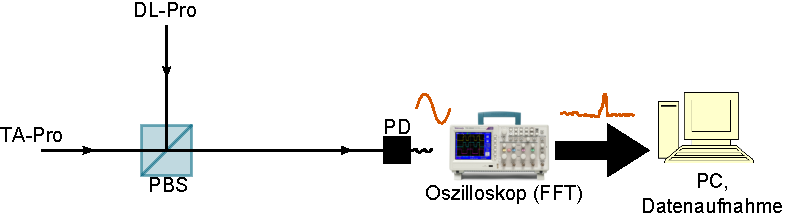
\includegraphics[width=\textwidth-2cm]{gfx/beatfrequenzmessung_aufbau_schematisch}
		}\\
 	\subfloat[]{
		\label{subfig:beatfrequenzen_signal}
		% GNUPLOT: LaTeX picture with Postscript
\begingroup
  \makeatletter
  \providecommand\color[2][]{%
    \GenericError{(gnuplot) \space\space\space\@spaces}{%
      Package color not loaded in conjunction with
      terminal option `colourtext'%
    }{See the gnuplot documentation for explanation.%
    }{Either use 'blacktext' in gnuplot or load the package
      color.sty in LaTeX.}%
    \renewcommand\color[2][]{}%
  }%
  \providecommand\includegraphics[2][]{%
    \GenericError{(gnuplot) \space\space\space\@spaces}{%
      Package graphicx or graphics not loaded%
    }{See the gnuplot documentation for explanation.%
    }{The gnuplot epslatex terminal needs graphicx.sty or graphics.sty.}%
    \renewcommand\includegraphics[2][]{}%
  }%
  \providecommand\rotatebox[2]{#2}%
  \@ifundefined{ifGPcolor}{%
    \newif\ifGPcolor
    \GPcolortrue
  }{}%
  \@ifundefined{ifGPblacktext}{%
    \newif\ifGPblacktext
    \GPblacktexttrue
  }{}%
  % define a \g@addto@macro without @ in the name:
  \let\gplgaddtomacro\g@addto@macro
  % define empty templates for all commands taking text:
  \gdef\gplbacktext{}%
  \gdef\gplfronttext{}%
  \makeatother
  \ifGPblacktext
    % no textcolor at all
    \def\colorrgb#1{}%
    \def\colorgray#1{}%
  \else
    % gray or color?
    \ifGPcolor
      \def\colorrgb#1{\color[rgb]{#1}}%
      \def\colorgray#1{\color[gray]{#1}}%
      \expandafter\def\csname LTw\endcsname{\color{white}}%
      \expandafter\def\csname LTb\endcsname{\color{black}}%
      \expandafter\def\csname LTa\endcsname{\color{black}}%
      \expandafter\def\csname LT0\endcsname{\color[rgb]{1,0,0}}%
      \expandafter\def\csname LT1\endcsname{\color[rgb]{0,1,0}}%
      \expandafter\def\csname LT2\endcsname{\color[rgb]{0,0,1}}%
      \expandafter\def\csname LT3\endcsname{\color[rgb]{1,0,1}}%
      \expandafter\def\csname LT4\endcsname{\color[rgb]{0,1,1}}%
      \expandafter\def\csname LT5\endcsname{\color[rgb]{1,1,0}}%
      \expandafter\def\csname LT6\endcsname{\color[rgb]{0,0,0}}%
      \expandafter\def\csname LT7\endcsname{\color[rgb]{1,0.3,0}}%
      \expandafter\def\csname LT8\endcsname{\color[rgb]{0.5,0.5,0.5}}%
    \else
      % gray
      \def\colorrgb#1{\color{black}}%
      \def\colorgray#1{\color[gray]{#1}}%
      \expandafter\def\csname LTw\endcsname{\color{white}}%
      \expandafter\def\csname LTb\endcsname{\color{black}}%
      \expandafter\def\csname LTa\endcsname{\color{black}}%
      \expandafter\def\csname LT0\endcsname{\color{black}}%
      \expandafter\def\csname LT1\endcsname{\color{black}}%
      \expandafter\def\csname LT2\endcsname{\color{black}}%
      \expandafter\def\csname LT3\endcsname{\color{black}}%
      \expandafter\def\csname LT4\endcsname{\color{black}}%
      \expandafter\def\csname LT5\endcsname{\color{black}}%
      \expandafter\def\csname LT6\endcsname{\color{black}}%
      \expandafter\def\csname LT7\endcsname{\color{black}}%
      \expandafter\def\csname LT8\endcsname{\color{black}}%
    \fi
  \fi
  \setlength{\unitlength}{0.0500bp}%
  \begin{picture}(7936.00,3968.00)%
    \gplgaddtomacro\gplbacktext{%
      \csname LTb\endcsname%
      \put(860,640){\makebox(0,0)[r]{\strut{}-3}}%
      \put(860,1010){\makebox(0,0)[r]{\strut{}-2.5}}%
      \put(860,1379){\makebox(0,0)[r]{\strut{}-2}}%
      \put(860,1749){\makebox(0,0)[r]{\strut{}-1.5}}%
      \put(860,2119){\makebox(0,0)[r]{\strut{}-1}}%
      \put(860,2488){\makebox(0,0)[r]{\strut{}-0.5}}%
      \put(860,2858){\makebox(0,0)[r]{\strut{} 0}}%
      \put(860,3228){\makebox(0,0)[r]{\strut{} 0.5}}%
      \put(860,3597){\makebox(0,0)[r]{\strut{} 1}}%
      \put(860,3967){\makebox(0,0)[r]{\strut{} 1.5}}%
      \put(980,440){\makebox(0,0){\strut{} 0}}%
      \put(1639,440){\makebox(0,0){\strut{} 50}}%
      \put(2299,440){\makebox(0,0){\strut{} 100}}%
      \put(2958,440){\makebox(0,0){\strut{} 150}}%
      \put(3618,440){\makebox(0,0){\strut{} 200}}%
      \put(4277,440){\makebox(0,0){\strut{} 250}}%
      \put(4937,440){\makebox(0,0){\strut{} 300}}%
      \put(5596,440){\makebox(0,0){\strut{} 350}}%
      \put(6256,440){\makebox(0,0){\strut{} 400}}%
      \put(6915,440){\makebox(0,0){\strut{} 450}}%
      \put(7575,440){\makebox(0,0){\strut{} 500}}%
      \put(160,2303){\rotatebox{-270}{\makebox(0,0){\strut{}Amplitude [mV]}}}%
      \put(4277,140){\makebox(0,0){\strut{}Zeit [ns]}}%
    }%
    \gplgaddtomacro\gplfronttext{%
    }%
    \gplbacktext
    \put(0,0){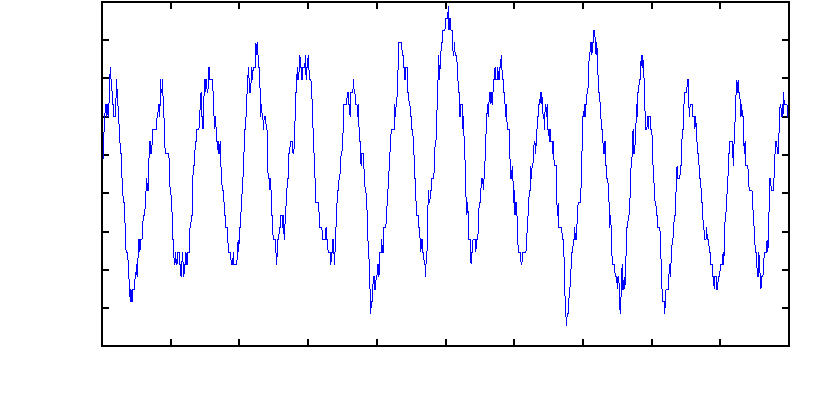
\includegraphics{beatfrequenzen_signal}}%
    \gplfronttext
  \end{picture}%
\endgroup

		}\\
	 \subfloat[]{
		\label{subfig:beatfrequenzen_fft}
		% GNUPLOT: LaTeX picture with Postscript
\begingroup
  \makeatletter
  \providecommand\color[2][]{%
    \GenericError{(gnuplot) \space\space\space\@spaces}{%
      Package color not loaded in conjunction with
      terminal option `colourtext'%
    }{See the gnuplot documentation for explanation.%
    }{Either use 'blacktext' in gnuplot or load the package
      color.sty in LaTeX.}%
    \renewcommand\color[2][]{}%
  }%
  \providecommand\includegraphics[2][]{%
    \GenericError{(gnuplot) \space\space\space\@spaces}{%
      Package graphicx or graphics not loaded%
    }{See the gnuplot documentation for explanation.%
    }{The gnuplot epslatex terminal needs graphicx.sty or graphics.sty.}%
    \renewcommand\includegraphics[2][]{}%
  }%
  \providecommand\rotatebox[2]{#2}%
  \@ifundefined{ifGPcolor}{%
    \newif\ifGPcolor
    \GPcolortrue
  }{}%
  \@ifundefined{ifGPblacktext}{%
    \newif\ifGPblacktext
    \GPblacktexttrue
  }{}%
  % define a \g@addto@macro without @ in the name:
  \let\gplgaddtomacro\g@addto@macro
  % define empty templates for all commands taking text:
  \gdef\gplbacktext{}%
  \gdef\gplfronttext{}%
  \makeatother
  \ifGPblacktext
    % no textcolor at all
    \def\colorrgb#1{}%
    \def\colorgray#1{}%
  \else
    % gray or color?
    \ifGPcolor
      \def\colorrgb#1{\color[rgb]{#1}}%
      \def\colorgray#1{\color[gray]{#1}}%
      \expandafter\def\csname LTw\endcsname{\color{white}}%
      \expandafter\def\csname LTb\endcsname{\color{black}}%
      \expandafter\def\csname LTa\endcsname{\color{black}}%
      \expandafter\def\csname LT0\endcsname{\color[rgb]{1,0,0}}%
      \expandafter\def\csname LT1\endcsname{\color[rgb]{0,1,0}}%
      \expandafter\def\csname LT2\endcsname{\color[rgb]{0,0,1}}%
      \expandafter\def\csname LT3\endcsname{\color[rgb]{1,0,1}}%
      \expandafter\def\csname LT4\endcsname{\color[rgb]{0,1,1}}%
      \expandafter\def\csname LT5\endcsname{\color[rgb]{1,1,0}}%
      \expandafter\def\csname LT6\endcsname{\color[rgb]{0,0,0}}%
      \expandafter\def\csname LT7\endcsname{\color[rgb]{1,0.3,0}}%
      \expandafter\def\csname LT8\endcsname{\color[rgb]{0.5,0.5,0.5}}%
    \else
      % gray
      \def\colorrgb#1{\color{black}}%
      \def\colorgray#1{\color[gray]{#1}}%
      \expandafter\def\csname LTw\endcsname{\color{white}}%
      \expandafter\def\csname LTb\endcsname{\color{black}}%
      \expandafter\def\csname LTa\endcsname{\color{black}}%
      \expandafter\def\csname LT0\endcsname{\color{black}}%
      \expandafter\def\csname LT1\endcsname{\color{black}}%
      \expandafter\def\csname LT2\endcsname{\color{black}}%
      \expandafter\def\csname LT3\endcsname{\color{black}}%
      \expandafter\def\csname LT4\endcsname{\color{black}}%
      \expandafter\def\csname LT5\endcsname{\color{black}}%
      \expandafter\def\csname LT6\endcsname{\color{black}}%
      \expandafter\def\csname LT7\endcsname{\color{black}}%
      \expandafter\def\csname LT8\endcsname{\color{black}}%
    \fi
  \fi
  \setlength{\unitlength}{0.0500bp}%
  \begin{picture}(7936.00,3968.00)%
    \gplgaddtomacro\gplbacktext{%
      \csname LTb\endcsname%
      \put(960,440){\makebox(0,0){\strut{} 0}}%
      \put(1622,440){\makebox(0,0){\strut{} 5}}%
      \put(2283,440){\makebox(0,0){\strut{} 10}}%
      \put(2945,440){\makebox(0,0){\strut{} 15}}%
      \put(3606,440){\makebox(0,0){\strut{} 20}}%
      \put(4268,440){\makebox(0,0){\strut{} 25}}%
      \put(4929,440){\makebox(0,0){\strut{} 30}}%
      \put(5591,440){\makebox(0,0){\strut{} 35}}%
      \put(6252,440){\makebox(0,0){\strut{} 40}}%
      \put(6914,440){\makebox(0,0){\strut{} 45}}%
      \put(7575,440){\makebox(0,0){\strut{} 50}}%
      \put(760,2293){\rotatebox{-270}{\makebox(0,0){\strut{}Amplitude}}}%
      \put(4267,140){\makebox(0,0){\strut{}Frequenz [MHz]}}%
      \put(1622,3616){\makebox(0,0)[l]{\strut{}$\sigma = (0.256\pm0.016)\,$MHz}}%
      \put(1622,3385){\makebox(0,0)[l]{\strut{}$\mu = (26.633\pm0.015)\,$MHz}}%
    }%
    \gplgaddtomacro\gplfronttext{%
      \csname LTb\endcsname%
      \put(6672,3784){\makebox(0,0)[r]{\strut{}Messpunkte}}%
      \csname LTb\endcsname%
      \put(6672,3584){\makebox(0,0)[r]{\strut{}Fit}}%
    }%
    \gplbacktext
    \put(0,0){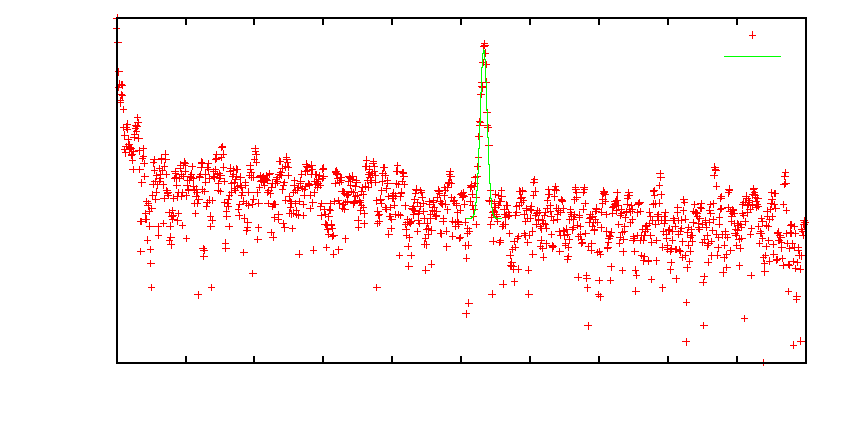
\includegraphics{beatfrequenzen_fft}}%
    \gplfronttext
  \end{picture}%
\endgroup

		}
	}}
	\caption[Beatfrequenzmessung]{(a) Aufbau der
	Schwebungsfrequenzmessung. (b) Schwebungssignal über einen
	Ausschnitt von $500\,$ns. (c) Fouriertransformierte dieses
	Signals. Weitere Erklärungen finden sich im Text. ((b) und (c) sind nur
	exemplarische Darstellungen und sind nicht miteinander korreliert.)}
	\label{fig:beatfrequenzmessung}
\end{figure}
Um die Aussagekraft der Messungen im vorherigen Abschnitt durch eine wesentlich
direktere Methode zur Relativfrequenzanalyse zu überprüfen, eignet sich hervorragend die
Messung von Schwebungsfrequenzen der beiden roten Laser. Dazu wurden wie in Abb.
\ref{fig:beatfrequenzmessung}\subref{subfig:beatfrequenzmessung_aufbau_schematisch}
schematisch dargestellt jeweils ein Teilstrahl der beiden Laser mit einen Polarisationsstrahlteiler
überlagert und auf eine Photodiode geschickt. Bringt man nun die Frequenzen
beider Laser auf nahe beieinander liegende Frequenzen (wenige MHz
Unterschied), entsteht durch Interferenz beider
elektromagnetischer Felder ein Schwebungssignal mit der Differenzfrequenz der
beiden Laserfrequenzen (siehe Abb.
\ref{fig:beatfrequenzmessung}\subref{subfig:beatfrequenzen_signal}). Das
Schwebungssignal kann durch den Strom der Photodiode an einem Oszilloskop über
die \textit{Fast-Fourier-Transformation} (FFT) spektral analysiert werden. Pro
Messung wurden so über einige Minuten mehrere $1000$ Frequenzspektren
aufgenommen, an die  mithilfe eines selbst geschriebenen \textit{Python}-Skripts
und \textit{GnuPlot} ein Gaußprofil angefittet wurde (siehe exemplarisch
\ref{fig:beatfrequenzmessung}\subref{subfig:beatfrequenzen_fft}).
Sowohl für das neue als auch für das alte System wurden bei stabilisierten
Lasern Schwebungssignale analysiert. Unstabilisiert ist es praktisch nicht
möglich einen Frequenzverlauf aufzuzeichnen, da die Laser schnell in zu
große Differenzfrequenzen driften. Zum einen bricht das Schwebungssignal
bei großen Schwebungsfrequnzen ($>30\,$MHz) fast völlig ein und kann nicht mehr
analysiert werden. Zum anderen treten Zweideutigkeiten auf, wenn die
Differenzfrequenz ihr Vorzeichen wechselt, was durchaus eintreten kann, wenn die
Laser zu Beginn in der Frequenz nur wenige MHz auseinander liegen.

\subsubsection{Schwebungsfrequenzen im neuen
System}\label{subsubsec:beatfrequenzmessung_neues_system}
Beim neuen System wurden die Schwebungsfrequenzen sowohl nur mit
\textit{iScan}-Stabilisierung als auch mit der Kombination von \textit{iScan}
und FOL aufgenommen.
\begin{figure}[hp]
 	\centering
 	\footnotesize
 	\fbox{\parbox{\dimexpr \linewidth - 2\fboxrule - 2\fboxsep}{
 	\subfloat[]{
		\label{subfig:beatfrequenzen_neu_iScan_drift}
		% GNUPLOT: LaTeX picture with Postscript
\begingroup
  \makeatletter
  \providecommand\color[2][]{%
    \GenericError{(gnuplot) \space\space\space\@spaces}{%
      Package color not loaded in conjunction with
      terminal option `colourtext'%
    }{See the gnuplot documentation for explanation.%
    }{Either use 'blacktext' in gnuplot or load the package
      color.sty in LaTeX.}%
    \renewcommand\color[2][]{}%
  }%
  \providecommand\includegraphics[2][]{%
    \GenericError{(gnuplot) \space\space\space\@spaces}{%
      Package graphicx or graphics not loaded%
    }{See the gnuplot documentation for explanation.%
    }{The gnuplot epslatex terminal needs graphicx.sty or graphics.sty.}%
    \renewcommand\includegraphics[2][]{}%
  }%
  \providecommand\rotatebox[2]{#2}%
  \@ifundefined{ifGPcolor}{%
    \newif\ifGPcolor
    \GPcolortrue
  }{}%
  \@ifundefined{ifGPblacktext}{%
    \newif\ifGPblacktext
    \GPblacktexttrue
  }{}%
  % define a \g@addto@macro without @ in the name:
  \let\gplgaddtomacro\g@addto@macro
  % define empty templates for all commands taking text:
  \gdef\gplbacktext{}%
  \gdef\gplfronttext{}%
  \makeatother
  \ifGPblacktext
    % no textcolor at all
    \def\colorrgb#1{}%
    \def\colorgray#1{}%
  \else
    % gray or color?
    \ifGPcolor
      \def\colorrgb#1{\color[rgb]{#1}}%
      \def\colorgray#1{\color[gray]{#1}}%
      \expandafter\def\csname LTw\endcsname{\color{white}}%
      \expandafter\def\csname LTb\endcsname{\color{black}}%
      \expandafter\def\csname LTa\endcsname{\color{black}}%
      \expandafter\def\csname LT0\endcsname{\color[rgb]{1,0,0}}%
      \expandafter\def\csname LT1\endcsname{\color[rgb]{0,1,0}}%
      \expandafter\def\csname LT2\endcsname{\color[rgb]{0,0,1}}%
      \expandafter\def\csname LT3\endcsname{\color[rgb]{1,0,1}}%
      \expandafter\def\csname LT4\endcsname{\color[rgb]{0,1,1}}%
      \expandafter\def\csname LT5\endcsname{\color[rgb]{1,1,0}}%
      \expandafter\def\csname LT6\endcsname{\color[rgb]{0,0,0}}%
      \expandafter\def\csname LT7\endcsname{\color[rgb]{1,0.3,0}}%
      \expandafter\def\csname LT8\endcsname{\color[rgb]{0.5,0.5,0.5}}%
    \else
      % gray
      \def\colorrgb#1{\color{black}}%
      \def\colorgray#1{\color[gray]{#1}}%
      \expandafter\def\csname LTw\endcsname{\color{white}}%
      \expandafter\def\csname LTb\endcsname{\color{black}}%
      \expandafter\def\csname LTa\endcsname{\color{black}}%
      \expandafter\def\csname LT0\endcsname{\color{black}}%
      \expandafter\def\csname LT1\endcsname{\color{black}}%
      \expandafter\def\csname LT2\endcsname{\color{black}}%
      \expandafter\def\csname LT3\endcsname{\color{black}}%
      \expandafter\def\csname LT4\endcsname{\color{black}}%
      \expandafter\def\csname LT5\endcsname{\color{black}}%
      \expandafter\def\csname LT6\endcsname{\color{black}}%
      \expandafter\def\csname LT7\endcsname{\color{black}}%
      \expandafter\def\csname LT8\endcsname{\color{black}}%
    \fi
  \fi
  \setlength{\unitlength}{0.0500bp}%
  \begin{picture}(7200.00,5040.00)%
    \gplgaddtomacro\gplbacktext{%
      \csname LTb\endcsname%
      \put(740,640){\makebox(0,0)[r]{\strut{} 0}}%
      \put(740,1333){\makebox(0,0)[r]{\strut{} 5}}%
      \put(740,2026){\makebox(0,0)[r]{\strut{} 10}}%
      \put(740,2719){\makebox(0,0)[r]{\strut{} 15}}%
      \put(740,3413){\makebox(0,0)[r]{\strut{} 20}}%
      \put(740,4106){\makebox(0,0)[r]{\strut{} 25}}%
      \put(740,4799){\makebox(0,0)[r]{\strut{} 30}}%
      \put(860,440){\makebox(0,0){\strut{} 0}}%
      \put(1524,440){\makebox(0,0){\strut{} 200}}%
      \put(2189,440){\makebox(0,0){\strut{} 400}}%
      \put(2853,440){\makebox(0,0){\strut{} 600}}%
      \put(3517,440){\makebox(0,0){\strut{} 800}}%
      \put(4182,440){\makebox(0,0){\strut{} 1000}}%
      \put(4846,440){\makebox(0,0){\strut{} 1200}}%
      \put(5510,440){\makebox(0,0){\strut{} 1400}}%
      \put(6175,440){\makebox(0,0){\strut{} 1600}}%
      \put(6839,440){\makebox(0,0){\strut{} 1800}}%
      \put(160,2719){\rotatebox{-270}{\makebox(0,0){\strut{}Schwebungsfrequenz [MHz]}}}%
      \put(3849,140){\makebox(0,0){\strut{}Messpunkt #}}%
    }%
    \gplgaddtomacro\gplfronttext{%
    }%
    \gplbacktext
    \put(0,0){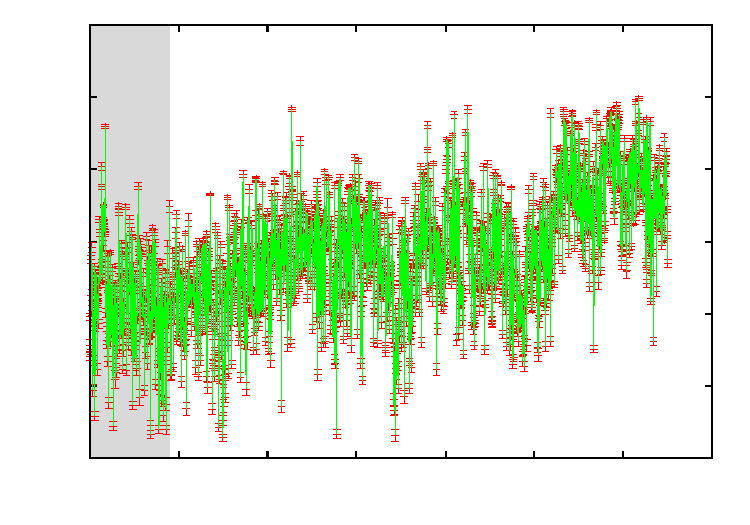
\includegraphics{beatfrequenzen_neu_iScan_drift}}%
    \gplfronttext
  \end{picture}%
\endgroup

		}\\
 	\subfloat[]{
		\label{subfig:beatfrequenzen_neu_iScan_histogramm}
		% GNUPLOT: LaTeX picture with Postscript
\begingroup
  \makeatletter
  \providecommand\color[2][]{%
    \GenericError{(gnuplot) \space\space\space\@spaces}{%
      Package color not loaded in conjunction with
      terminal option `colourtext'%
    }{See the gnuplot documentation for explanation.%
    }{Either use 'blacktext' in gnuplot or load the package
      color.sty in LaTeX.}%
    \renewcommand\color[2][]{}%
  }%
  \providecommand\includegraphics[2][]{%
    \GenericError{(gnuplot) \space\space\space\@spaces}{%
      Package graphicx or graphics not loaded%
    }{See the gnuplot documentation for explanation.%
    }{The gnuplot epslatex terminal needs graphicx.sty or graphics.sty.}%
    \renewcommand\includegraphics[2][]{}%
  }%
  \providecommand\rotatebox[2]{#2}%
  \@ifundefined{ifGPcolor}{%
    \newif\ifGPcolor
    \GPcolortrue
  }{}%
  \@ifundefined{ifGPblacktext}{%
    \newif\ifGPblacktext
    \GPblacktexttrue
  }{}%
  % define a \g@addto@macro without @ in the name:
  \let\gplgaddtomacro\g@addto@macro
  % define empty templates for all commands taking text:
  \gdef\gplbacktext{}%
  \gdef\gplfronttext{}%
  \makeatother
  \ifGPblacktext
    % no textcolor at all
    \def\colorrgb#1{}%
    \def\colorgray#1{}%
  \else
    % gray or color?
    \ifGPcolor
      \def\colorrgb#1{\color[rgb]{#1}}%
      \def\colorgray#1{\color[gray]{#1}}%
      \expandafter\def\csname LTw\endcsname{\color{white}}%
      \expandafter\def\csname LTb\endcsname{\color{black}}%
      \expandafter\def\csname LTa\endcsname{\color{black}}%
      \expandafter\def\csname LT0\endcsname{\color[rgb]{1,0,0}}%
      \expandafter\def\csname LT1\endcsname{\color[rgb]{0,1,0}}%
      \expandafter\def\csname LT2\endcsname{\color[rgb]{0,0,1}}%
      \expandafter\def\csname LT3\endcsname{\color[rgb]{1,0,1}}%
      \expandafter\def\csname LT4\endcsname{\color[rgb]{0,1,1}}%
      \expandafter\def\csname LT5\endcsname{\color[rgb]{1,1,0}}%
      \expandafter\def\csname LT6\endcsname{\color[rgb]{0,0,0}}%
      \expandafter\def\csname LT7\endcsname{\color[rgb]{1,0.3,0}}%
      \expandafter\def\csname LT8\endcsname{\color[rgb]{0.5,0.5,0.5}}%
    \else
      % gray
      \def\colorrgb#1{\color{black}}%
      \def\colorgray#1{\color[gray]{#1}}%
      \expandafter\def\csname LTw\endcsname{\color{white}}%
      \expandafter\def\csname LTb\endcsname{\color{black}}%
      \expandafter\def\csname LTa\endcsname{\color{black}}%
      \expandafter\def\csname LT0\endcsname{\color{black}}%
      \expandafter\def\csname LT1\endcsname{\color{black}}%
      \expandafter\def\csname LT2\endcsname{\color{black}}%
      \expandafter\def\csname LT3\endcsname{\color{black}}%
      \expandafter\def\csname LT4\endcsname{\color{black}}%
      \expandafter\def\csname LT5\endcsname{\color{black}}%
      \expandafter\def\csname LT6\endcsname{\color{black}}%
      \expandafter\def\csname LT7\endcsname{\color{black}}%
      \expandafter\def\csname LT8\endcsname{\color{black}}%
    \fi
  \fi
  \setlength{\unitlength}{0.0500bp}%
  \begin{picture}(7200.00,5040.00)%
    \gplgaddtomacro\gplbacktext{%
      \csname LTb\endcsname%
      \put(740,640){\makebox(0,0)[r]{\strut{} 0}}%
      \put(740,1234){\makebox(0,0)[r]{\strut{} 10}}%
      \put(740,1828){\makebox(0,0)[r]{\strut{} 20}}%
      \put(740,2422){\makebox(0,0)[r]{\strut{} 30}}%
      \put(740,3017){\makebox(0,0)[r]{\strut{} 40}}%
      \put(740,3611){\makebox(0,0)[r]{\strut{} 50}}%
      \put(740,4205){\makebox(0,0)[r]{\strut{} 60}}%
      \put(740,4799){\makebox(0,0)[r]{\strut{} 70}}%
      \put(860,440){\makebox(0,0){\strut{} 0}}%
      \put(2056,440){\makebox(0,0){\strut{} 5}}%
      \put(3252,440){\makebox(0,0){\strut{} 10}}%
      \put(4447,440){\makebox(0,0){\strut{} 15}}%
      \put(5643,440){\makebox(0,0){\strut{} 20}}%
      \put(6839,440){\makebox(0,0){\strut{} 25}}%
      \put(160,2719){\rotatebox{-270}{\makebox(0,0){\strut{}H"aufigkeit}}}%
      \put(3849,140){\makebox(0,0){\strut{}Schwebungsfrequenz [MHz]}}%
      \put(4148,4591){\makebox(0,0)[l]{\strut{}$\sigma = (3.10\pm0.11)\,$MHz}}%
      \put(4148,4300){\makebox(0,0)[l]{\strut{}$A = (423\pm14)\,$MHz}}%
      \put(4148,4009){\makebox(0,0)[l]{\strut{}$\mu = (10.54\pm0.11)\,$MHz}}%
    }%
    \gplgaddtomacro\gplfronttext{%
    }%
    \gplbacktext
    \put(0,0){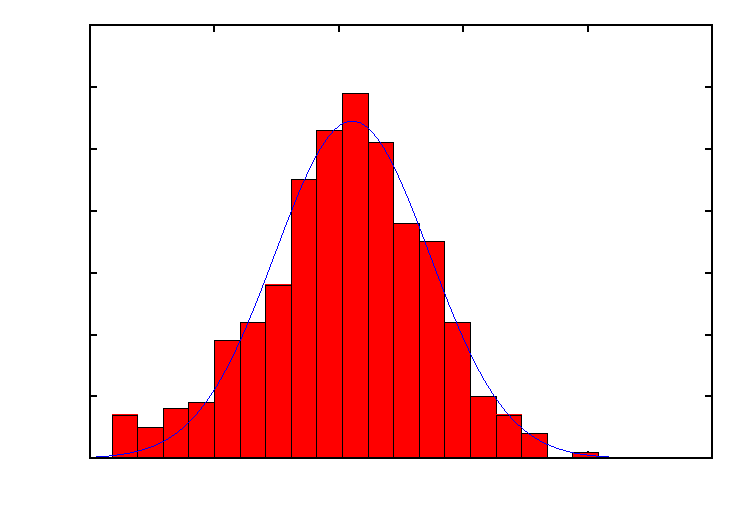
\includegraphics{beatfrequenzen_neu_iScan_histogramm}}%
    \gplfronttext
  \end{picture}%
\endgroup

		}
	}}
	\caption[Beatfrequenzen - neues System mit \textit{iScan}]{(a) Frequenzverlauf
	des Schwebungssignals der beiden roten \textit{iScan}-stabilisierten Laser des neuen Systems über eine Zeit von
	$65\,$min. (b) zeigt die Frequenzverteilung in den ersten $9\,$min der
	Messung (grauer Bereich in (a)).}
	\label{fig:beatfrequenzen_neu_iScan}
\end{figure}
Abbildung
\ref{fig:beatfrequenzen_neu_iScan}\subref{subfig:beatfrequenzen_neu_iScan_drift} zeigt den Frequenzverlauf des Schwebungssignals über einen Zeitraum von $65\,$min mit
\textit{iScan}-Regelung. Die Fehlerbalken resultieren aus den
Standardabweichungen der einzelnen Gauß-Fits. Es ist eine leichte Drift von
maximal $10\,$MHz zu erkennen, welcher in der Größenordnung mit den
einzelnen Drifts der beiden Laser bei den Messungen des vorherigen Abschnitts
übereinstimmt. Dort sind die beide Laser jeweils in der gleichen Zeit ca.
$10\,$MHz gedriftet. Zu beachten ist, dass synchrone Drifts beider Laser (evtl.
Temperaturdrifts) keine Auswirkungen auf Schwebungsfrequenzdrifts haben. Um eine
quantitativ gesicherte Aussage über den Vergleich beider Messungen machen zu
können, wären viele Einzelmessungen mit guter Statistik sowie ggf. eine
systematische Beeinflussung der Schwebung über äußere Einflüsse nötig.
Die Messung der Schwebungsfrequenzen liefert also bezüglich der Drift qualitativ die gleiche
Aussage wie die Messungen mit der neuen Software. Weiterhin kann eine quantitative Aussage über die Fluktuation
der Laserfrequenzen in kleinen Zeitskalen bei eingeschalteter
\textit{iScan}-Stabilisierung getroffen werden. Dazu wurde für die ersten
$9\,$min der Messung (grauer Bereich in Abb.
\ref{fig:beatfrequenzen_neu_iScan}\subref{subfig:beatfrequenzen_neu_iScan_drift})
eine Analyse der Frequenzverteilung durchgeführt (siehe Abb.
\ref{fig:beatfrequenzen_neu_iScan}\subref{subfig:beatfrequenzen_neu_iScan_histogramm}).
In diesem Zeitraum waren die Laser noch fast keiner Drift unterworfen. Die Lücke
im niederfrequenten Bereich des Histogramms resultiert aus der
Frequenzauflösungsbeschränkung des Oszilloskops. An das Histogramm wurde eine
Gaußkurve gemäß
\begin{equation}\label{eq:schwebungsfrequenzen_gauss}
	G(\nu)=A\cdot\frac{1}{\sigma\sqrt{2\pi}}\mathrm{e}^{-\frac{1}{2}\frac{(\nu-\mu)^2}{\sigma^2}}
\end{equation}
angepasst. Man findet $2\sigma_{ges,neu,iScan}=(6,20\pm0,23)\,$MHz als
Standardabweichung und gleichzeitig als Linienbreite der Faltung der effektiven Linienbreiten beider
Laser\footnote{In die effektive Linienbreite fließen hier neben der Linienbreite
des ungestörten Lasers noch alle durch äußere Störungen verursachten
Frequenzfluktuationen ein.}. Geht man davon aus, dass die effektiven
Linienbreiten der Laser in etwa gleich sind, findet man über
\begin{equation}\label{eq:schwebungsfrequenzen_linienbreite}
	\sigma_{ges}=\sqrt{\sigma_1^2+\sigma_2^2}
\end{equation}
die effektiven Linienbreiten der beiden Laser
$2\sigma_{1,neu,iScan}=2\sigma_{2,neu,iScan}=(4,38\pm0,16)\,$MHz. Diese ist
wichtig, um bei weiterführenden spektroskopischen Messungen Aussagen über
Übergangslinienbreiten treffen zu können.\par
Abbildung \ref{fig:beatfrequenzen_neu_iScan+FOL} zeigt die
Schwebungsfrequenzmessung mit \textit{iScan}+FOL-Stabilisierung.
\begin{figure}[hp]
 	\centering
 	\footnotesize
 	\fbox{\parbox{\dimexpr \linewidth - 2\fboxrule - 2\fboxsep}{
 	\subfloat[]{
		\label{subfig:beatfrequenzen_neu_iScan+FOL_drift}
		% GNUPLOT: LaTeX picture with Postscript
\begingroup
  \makeatletter
  \providecommand\color[2][]{%
    \GenericError{(gnuplot) \space\space\space\@spaces}{%
      Package color not loaded in conjunction with
      terminal option `colourtext'%
    }{See the gnuplot documentation for explanation.%
    }{Either use 'blacktext' in gnuplot or load the package
      color.sty in LaTeX.}%
    \renewcommand\color[2][]{}%
  }%
  \providecommand\includegraphics[2][]{%
    \GenericError{(gnuplot) \space\space\space\@spaces}{%
      Package graphicx or graphics not loaded%
    }{See the gnuplot documentation for explanation.%
    }{The gnuplot epslatex terminal needs graphicx.sty or graphics.sty.}%
    \renewcommand\includegraphics[2][]{}%
  }%
  \providecommand\rotatebox[2]{#2}%
  \@ifundefined{ifGPcolor}{%
    \newif\ifGPcolor
    \GPcolortrue
  }{}%
  \@ifundefined{ifGPblacktext}{%
    \newif\ifGPblacktext
    \GPblacktexttrue
  }{}%
  % define a \g@addto@macro without @ in the name:
  \let\gplgaddtomacro\g@addto@macro
  % define empty templates for all commands taking text:
  \gdef\gplbacktext{}%
  \gdef\gplfronttext{}%
  \makeatother
  \ifGPblacktext
    % no textcolor at all
    \def\colorrgb#1{}%
    \def\colorgray#1{}%
  \else
    % gray or color?
    \ifGPcolor
      \def\colorrgb#1{\color[rgb]{#1}}%
      \def\colorgray#1{\color[gray]{#1}}%
      \expandafter\def\csname LTw\endcsname{\color{white}}%
      \expandafter\def\csname LTb\endcsname{\color{black}}%
      \expandafter\def\csname LTa\endcsname{\color{black}}%
      \expandafter\def\csname LT0\endcsname{\color[rgb]{1,0,0}}%
      \expandafter\def\csname LT1\endcsname{\color[rgb]{0,1,0}}%
      \expandafter\def\csname LT2\endcsname{\color[rgb]{0,0,1}}%
      \expandafter\def\csname LT3\endcsname{\color[rgb]{1,0,1}}%
      \expandafter\def\csname LT4\endcsname{\color[rgb]{0,1,1}}%
      \expandafter\def\csname LT5\endcsname{\color[rgb]{1,1,0}}%
      \expandafter\def\csname LT6\endcsname{\color[rgb]{0,0,0}}%
      \expandafter\def\csname LT7\endcsname{\color[rgb]{1,0.3,0}}%
      \expandafter\def\csname LT8\endcsname{\color[rgb]{0.5,0.5,0.5}}%
    \else
      % gray
      \def\colorrgb#1{\color{black}}%
      \def\colorgray#1{\color[gray]{#1}}%
      \expandafter\def\csname LTw\endcsname{\color{white}}%
      \expandafter\def\csname LTb\endcsname{\color{black}}%
      \expandafter\def\csname LTa\endcsname{\color{black}}%
      \expandafter\def\csname LT0\endcsname{\color{black}}%
      \expandafter\def\csname LT1\endcsname{\color{black}}%
      \expandafter\def\csname LT2\endcsname{\color{black}}%
      \expandafter\def\csname LT3\endcsname{\color{black}}%
      \expandafter\def\csname LT4\endcsname{\color{black}}%
      \expandafter\def\csname LT5\endcsname{\color{black}}%
      \expandafter\def\csname LT6\endcsname{\color{black}}%
      \expandafter\def\csname LT7\endcsname{\color{black}}%
      \expandafter\def\csname LT8\endcsname{\color{black}}%
    \fi
  \fi
  \setlength{\unitlength}{0.0500bp}%
  \begin{picture}(7200.00,5040.00)%
    \gplgaddtomacro\gplbacktext{%
      \csname LTb\endcsname%
      \put(740,640){\makebox(0,0)[r]{\strut{} 5}}%
      \put(740,1160){\makebox(0,0)[r]{\strut{} 10}}%
      \put(740,1680){\makebox(0,0)[r]{\strut{} 15}}%
      \put(740,2200){\makebox(0,0)[r]{\strut{} 20}}%
      \put(740,2719){\makebox(0,0)[r]{\strut{} 25}}%
      \put(740,3239){\makebox(0,0)[r]{\strut{} 30}}%
      \put(740,3759){\makebox(0,0)[r]{\strut{} 35}}%
      \put(740,4279){\makebox(0,0)[r]{\strut{} 40}}%
      \put(740,4799){\makebox(0,0)[r]{\strut{} 45}}%
      \put(860,440){\makebox(0,0){\strut{} 0}}%
      \put(1607,440){\makebox(0,0){\strut{} 10}}%
      \put(2355,440){\makebox(0,0){\strut{} 20}}%
      \put(3102,440){\makebox(0,0){\strut{} 30}}%
      \put(3849,440){\makebox(0,0){\strut{} 40}}%
      \put(4597,440){\makebox(0,0){\strut{} 50}}%
      \put(5344,440){\makebox(0,0){\strut{} 60}}%
      \put(6092,440){\makebox(0,0){\strut{} 70}}%
      \put(6839,440){\makebox(0,0){\strut{} 80}}%
      \put(160,2719){\rotatebox{-270}{\makebox(0,0){\strut{}Schwebungsfrequenz [MHz]}}}%
      \put(3849,140){\makebox(0,0){\strut{}Zeit [min]}}%
    }%
    \gplgaddtomacro\gplfronttext{%
      \csname LTb\endcsname%
      \put(2056,1264){\makebox(0,0)[l]{\strut{}\textit{iScans}: aktiv}}%
      \put(2056,973){\makebox(0,0)[l]{\strut{}FOL: aktiv}}%
      \put(5045,1264){\makebox(0,0)[l]{\strut{}\textit{iScans}: aktiv}}%
      \put(5045,973){\makebox(0,0)[l]{\strut{}FOL: inaktiv}}%
    }%
    \gplbacktext
    \put(0,0){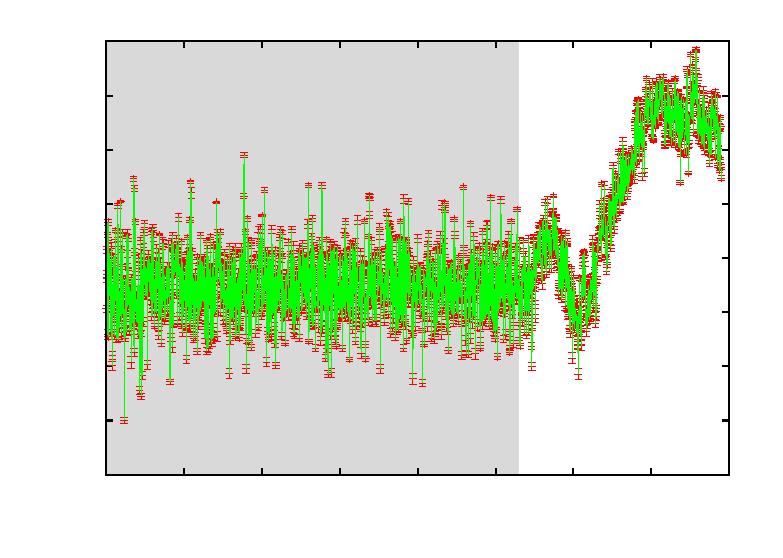
\includegraphics{beatfrequenzen_neu_iScan+FOL_drift}}%
    \gplfronttext
  \end{picture}%
\endgroup

		}\\
 	\subfloat[]{
		\label{subfig:beatfrequenzen_neu_iScan+FOL_histogramm}
		% GNUPLOT: LaTeX picture with Postscript
\begingroup
  \makeatletter
  \providecommand\color[2][]{%
    \GenericError{(gnuplot) \space\space\space\@spaces}{%
      Package color not loaded in conjunction with
      terminal option `colourtext'%
    }{See the gnuplot documentation for explanation.%
    }{Either use 'blacktext' in gnuplot or load the package
      color.sty in LaTeX.}%
    \renewcommand\color[2][]{}%
  }%
  \providecommand\includegraphics[2][]{%
    \GenericError{(gnuplot) \space\space\space\@spaces}{%
      Package graphicx or graphics not loaded%
    }{See the gnuplot documentation for explanation.%
    }{The gnuplot epslatex terminal needs graphicx.sty or graphics.sty.}%
    \renewcommand\includegraphics[2][]{}%
  }%
  \providecommand\rotatebox[2]{#2}%
  \@ifundefined{ifGPcolor}{%
    \newif\ifGPcolor
    \GPcolortrue
  }{}%
  \@ifundefined{ifGPblacktext}{%
    \newif\ifGPblacktext
    \GPblacktexttrue
  }{}%
  % define a \g@addto@macro without @ in the name:
  \let\gplgaddtomacro\g@addto@macro
  % define empty templates for all commands taking text:
  \gdef\gplbacktext{}%
  \gdef\gplfronttext{}%
  \makeatother
  \ifGPblacktext
    % no textcolor at all
    \def\colorrgb#1{}%
    \def\colorgray#1{}%
  \else
    % gray or color?
    \ifGPcolor
      \def\colorrgb#1{\color[rgb]{#1}}%
      \def\colorgray#1{\color[gray]{#1}}%
      \expandafter\def\csname LTw\endcsname{\color{white}}%
      \expandafter\def\csname LTb\endcsname{\color{black}}%
      \expandafter\def\csname LTa\endcsname{\color{black}}%
      \expandafter\def\csname LT0\endcsname{\color[rgb]{1,0,0}}%
      \expandafter\def\csname LT1\endcsname{\color[rgb]{0,1,0}}%
      \expandafter\def\csname LT2\endcsname{\color[rgb]{0,0,1}}%
      \expandafter\def\csname LT3\endcsname{\color[rgb]{1,0,1}}%
      \expandafter\def\csname LT4\endcsname{\color[rgb]{0,1,1}}%
      \expandafter\def\csname LT5\endcsname{\color[rgb]{1,1,0}}%
      \expandafter\def\csname LT6\endcsname{\color[rgb]{0,0,0}}%
      \expandafter\def\csname LT7\endcsname{\color[rgb]{1,0.3,0}}%
      \expandafter\def\csname LT8\endcsname{\color[rgb]{0.5,0.5,0.5}}%
    \else
      % gray
      \def\colorrgb#1{\color{black}}%
      \def\colorgray#1{\color[gray]{#1}}%
      \expandafter\def\csname LTw\endcsname{\color{white}}%
      \expandafter\def\csname LTb\endcsname{\color{black}}%
      \expandafter\def\csname LTa\endcsname{\color{black}}%
      \expandafter\def\csname LT0\endcsname{\color{black}}%
      \expandafter\def\csname LT1\endcsname{\color{black}}%
      \expandafter\def\csname LT2\endcsname{\color{black}}%
      \expandafter\def\csname LT3\endcsname{\color{black}}%
      \expandafter\def\csname LT4\endcsname{\color{black}}%
      \expandafter\def\csname LT5\endcsname{\color{black}}%
      \expandafter\def\csname LT6\endcsname{\color{black}}%
      \expandafter\def\csname LT7\endcsname{\color{black}}%
      \expandafter\def\csname LT8\endcsname{\color{black}}%
    \fi
  \fi
  \setlength{\unitlength}{0.0500bp}%
  \begin{picture}(7200.00,5040.00)%
    \gplgaddtomacro\gplbacktext{%
      \csname LTb\endcsname%
      \put(860,640){\makebox(0,0)[r]{\strut{} 0}}%
      \put(860,1160){\makebox(0,0)[r]{\strut{} 20}}%
      \put(860,1680){\makebox(0,0)[r]{\strut{} 40}}%
      \put(860,2200){\makebox(0,0)[r]{\strut{} 60}}%
      \put(860,2719){\makebox(0,0)[r]{\strut{} 80}}%
      \put(860,3239){\makebox(0,0)[r]{\strut{} 100}}%
      \put(860,3759){\makebox(0,0)[r]{\strut{} 120}}%
      \put(860,4279){\makebox(0,0)[r]{\strut{} 140}}%
      \put(860,4799){\makebox(0,0)[r]{\strut{} 160}}%
      \put(980,440){\makebox(0,0){\strut{} 5}}%
      \put(1957,440){\makebox(0,0){\strut{} 10}}%
      \put(2933,440){\makebox(0,0){\strut{} 15}}%
      \put(3910,440){\makebox(0,0){\strut{} 20}}%
      \put(4886,440){\makebox(0,0){\strut{} 25}}%
      \put(5863,440){\makebox(0,0){\strut{} 30}}%
      \put(6839,440){\makebox(0,0){\strut{} 35}}%
      \put(160,2719){\rotatebox{-270}{\makebox(0,0){\strut{}H"aufigkeit}}}%
      \put(3909,140){\makebox(0,0){\strut{}Schwebungsfrequenz [MHz]}}%
      \put(1273,4591){\makebox(0,0)[l]{\strut{}$\sigma = (2.780\pm0.070)\,$MHz}}%
      \put(1273,4300){\makebox(0,0)[l]{\strut{}$A = (899\pm20)\,$MHz}}%
      \put(1273,4009){\makebox(0,0)[l]{\strut{}$\mu = (22.035\pm0.070)\,$MHz}}%
    }%
    \gplgaddtomacro\gplfronttext{%
    }%
    \gplbacktext
    \put(0,0){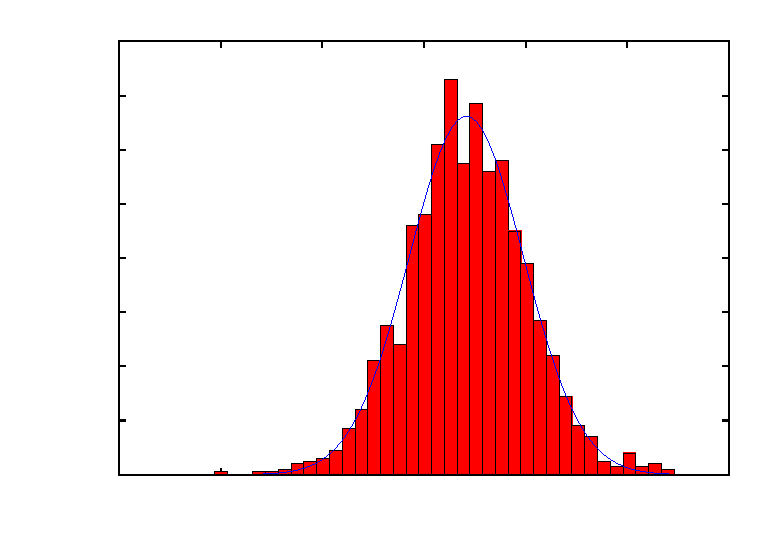
\includegraphics{beatfrequenzen_neu_iScan+FOL_histogramm}}%
    \gplfronttext
  \end{picture}%
\endgroup

		}
	}}
	\caption[Beatfrequenzen - neues System mit \textit{iScan}+FOL]{(a)
	Frequenzverlauf des Schwebungssignals der beiden roten
	\textit{iScan}+FOL-stabilisierten Laser des neuen Systems über eine Zeit von
	$79\,$min. Nach $53\,$min wurde das FOL allerdings ausgeschaltet, um
	einen direkten Vergleich zur alleinigen \textit{iScan}-Stabilisierung zu
	bekommen. (b) zeigt die Frequenzverteilung in den ersten $53\,$min der Messung
	(grauer Bereich in (a)), während die \textit{iScan}+FOL-Stabilisierung noch
	aktiv war.}
	\label{fig:beatfrequenzen_neu_iScan+FOL}
\end{figure}
Das FOL war in den ersten $53\,$min hinzugeschaltet und wurde danach
deaktiviert, die \textit{iScans} blieben aktiv. Während der aktiven Phase des
FOL (grauer Bereich in Abb.
\ref{fig:beatfrequenzen_neu_iScan+FOL}\subref{subfig:beatfrequenzen_neu_iScan+FOL_drift})
blieb die Schwebungsfrequenz weitgehendst konstant, was die korrekte Funktion des FOL bestätigt. Nach
Abschalten des FOL driften beide Laser auseinander. Für den
\textit{iScan}+FOL-stabilisierten Fall wurde wieder die Frequenzverteilung
analysiert, woraus eine Linienbreite von
$2\sigma_{ges,neu,iScan+FOL}=(5,56\pm0,14)\,$MHz hervorgeht. Für die effektive
Linienbreite der Laser folgt
$2\sigma_{1,neu,iScan+FOL}=2\sigma_{2,neu,iScan+FOL}=(3,93\pm0,10)\,$MHz mit
der Annahme, dass beide Laser annähernd die gleiche effektive Linienbreite haben.
Offensichtlich reduziert also das FOL zusätzlich zu den \textit{iScans} die
effektive Linienbreite der Laser geringfügig, wobei zu beachten ist, dass im
ersten Fall die Linienbreite fälschlicherweise verbreitert gemessen wurde. In der
Praxis hat also das Zuschalten des FOL keinen nennenswerten Effekt auf die
effektive Linienbreite in kleinen Zeitskalen.

\subsubsection{Schwebungsfrequenzen im alten
System}\label{subsubsec:beatfrequenzmessung_altes_system}
Abbildung \ref{fig:beatfrequenzen_alt_FOL} stellt das Verhalten der
Schwebungsfrequenz der beiden roten Laser im alten System über $30\,$min dar.
Auch hier wurde eine Frequenzverteilungsanalyse durchgeführt, allerdings über
den Zeitraum der kompletten Messung.
\begin{figure}[hp]
 	\centering
 	\footnotesize
 	\fbox{\parbox{\dimexpr \linewidth - 2\fboxrule - 2\fboxsep}{
 	\subfloat[]{
		\label{subfig:beatfrequenzen_alt_FOL_drift}
		% GNUPLOT: LaTeX picture with Postscript
\begingroup
  \makeatletter
  \providecommand\color[2][]{%
    \GenericError{(gnuplot) \space\space\space\@spaces}{%
      Package color not loaded in conjunction with
      terminal option `colourtext'%
    }{See the gnuplot documentation for explanation.%
    }{Either use 'blacktext' in gnuplot or load the package
      color.sty in LaTeX.}%
    \renewcommand\color[2][]{}%
  }%
  \providecommand\includegraphics[2][]{%
    \GenericError{(gnuplot) \space\space\space\@spaces}{%
      Package graphicx or graphics not loaded%
    }{See the gnuplot documentation for explanation.%
    }{The gnuplot epslatex terminal needs graphicx.sty or graphics.sty.}%
    \renewcommand\includegraphics[2][]{}%
  }%
  \providecommand\rotatebox[2]{#2}%
  \@ifundefined{ifGPcolor}{%
    \newif\ifGPcolor
    \GPcolortrue
  }{}%
  \@ifundefined{ifGPblacktext}{%
    \newif\ifGPblacktext
    \GPblacktexttrue
  }{}%
  % define a \g@addto@macro without @ in the name:
  \let\gplgaddtomacro\g@addto@macro
  % define empty templates for all commands taking text:
  \gdef\gplbacktext{}%
  \gdef\gplfronttext{}%
  \makeatother
  \ifGPblacktext
    % no textcolor at all
    \def\colorrgb#1{}%
    \def\colorgray#1{}%
  \else
    % gray or color?
    \ifGPcolor
      \def\colorrgb#1{\color[rgb]{#1}}%
      \def\colorgray#1{\color[gray]{#1}}%
      \expandafter\def\csname LTw\endcsname{\color{white}}%
      \expandafter\def\csname LTb\endcsname{\color{black}}%
      \expandafter\def\csname LTa\endcsname{\color{black}}%
      \expandafter\def\csname LT0\endcsname{\color[rgb]{1,0,0}}%
      \expandafter\def\csname LT1\endcsname{\color[rgb]{0,1,0}}%
      \expandafter\def\csname LT2\endcsname{\color[rgb]{0,0,1}}%
      \expandafter\def\csname LT3\endcsname{\color[rgb]{1,0,1}}%
      \expandafter\def\csname LT4\endcsname{\color[rgb]{0,1,1}}%
      \expandafter\def\csname LT5\endcsname{\color[rgb]{1,1,0}}%
      \expandafter\def\csname LT6\endcsname{\color[rgb]{0,0,0}}%
      \expandafter\def\csname LT7\endcsname{\color[rgb]{1,0.3,0}}%
      \expandafter\def\csname LT8\endcsname{\color[rgb]{0.5,0.5,0.5}}%
    \else
      % gray
      \def\colorrgb#1{\color{black}}%
      \def\colorgray#1{\color[gray]{#1}}%
      \expandafter\def\csname LTw\endcsname{\color{white}}%
      \expandafter\def\csname LTb\endcsname{\color{black}}%
      \expandafter\def\csname LTa\endcsname{\color{black}}%
      \expandafter\def\csname LT0\endcsname{\color{black}}%
      \expandafter\def\csname LT1\endcsname{\color{black}}%
      \expandafter\def\csname LT2\endcsname{\color{black}}%
      \expandafter\def\csname LT3\endcsname{\color{black}}%
      \expandafter\def\csname LT4\endcsname{\color{black}}%
      \expandafter\def\csname LT5\endcsname{\color{black}}%
      \expandafter\def\csname LT6\endcsname{\color{black}}%
      \expandafter\def\csname LT7\endcsname{\color{black}}%
      \expandafter\def\csname LT8\endcsname{\color{black}}%
    \fi
  \fi
  \setlength{\unitlength}{0.0500bp}%
  \begin{picture}(7200.00,5040.00)%
    \gplgaddtomacro\gplbacktext{%
      \csname LTb\endcsname%
      \put(740,640){\makebox(0,0)[r]{\strut{}-20}}%
      \put(740,1234){\makebox(0,0)[r]{\strut{}-10}}%
      \put(740,1828){\makebox(0,0)[r]{\strut{} 0}}%
      \put(740,2422){\makebox(0,0)[r]{\strut{} 10}}%
      \put(740,3017){\makebox(0,0)[r]{\strut{} 20}}%
      \put(740,3611){\makebox(0,0)[r]{\strut{} 30}}%
      \put(740,4205){\makebox(0,0)[r]{\strut{} 40}}%
      \put(740,4799){\makebox(0,0)[r]{\strut{} 50}}%
      \put(860,440){\makebox(0,0){\strut{} 0}}%
      \put(1857,440){\makebox(0,0){\strut{} 5}}%
      \put(2853,440){\makebox(0,0){\strut{} 10}}%
      \put(3850,440){\makebox(0,0){\strut{} 15}}%
      \put(4846,440){\makebox(0,0){\strut{} 20}}%
      \put(5843,440){\makebox(0,0){\strut{} 25}}%
      \put(6839,440){\makebox(0,0){\strut{} 30}}%
      \put(160,2719){\rotatebox{-270}{\makebox(0,0){\strut{}Schwebungsfrequenz [MHz]}}}%
      \put(3849,140){\makebox(0,0){\strut{}Zeit [min]}}%
    }%
    \gplgaddtomacro\gplfronttext{%
    }%
    \gplbacktext
    \put(0,0){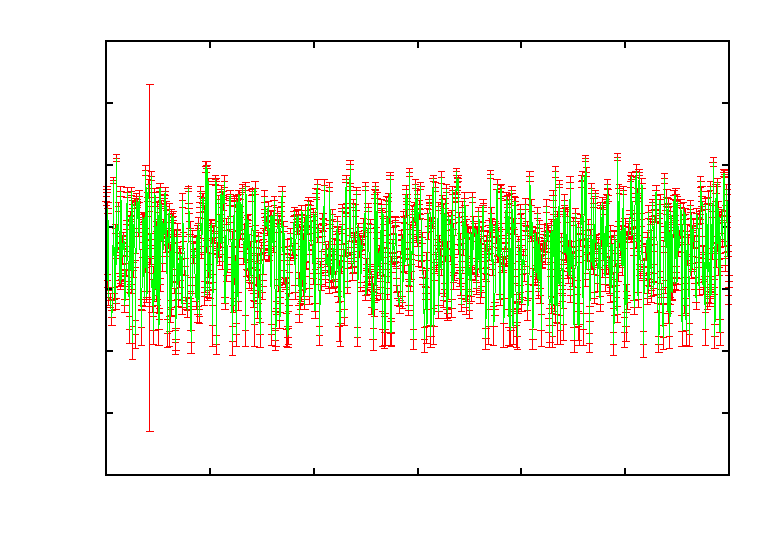
\includegraphics{beatfrequenzen_alt_FOL_drift}}%
    \gplfronttext
  \end{picture}%
\endgroup

		}\\
 	\subfloat[]{
		\label{subfig:beatfrequenzen_alt_FOL_histogramm}
		% GNUPLOT: LaTeX picture with Postscript
\begingroup
  \makeatletter
  \providecommand\color[2][]{%
    \GenericError{(gnuplot) \space\space\space\@spaces}{%
      Package color not loaded in conjunction with
      terminal option `colourtext'%
    }{See the gnuplot documentation for explanation.%
    }{Either use 'blacktext' in gnuplot or load the package
      color.sty in LaTeX.}%
    \renewcommand\color[2][]{}%
  }%
  \providecommand\includegraphics[2][]{%
    \GenericError{(gnuplot) \space\space\space\@spaces}{%
      Package graphicx or graphics not loaded%
    }{See the gnuplot documentation for explanation.%
    }{The gnuplot epslatex terminal needs graphicx.sty or graphics.sty.}%
    \renewcommand\includegraphics[2][]{}%
  }%
  \providecommand\rotatebox[2]{#2}%
  \@ifundefined{ifGPcolor}{%
    \newif\ifGPcolor
    \GPcolortrue
  }{}%
  \@ifundefined{ifGPblacktext}{%
    \newif\ifGPblacktext
    \GPblacktexttrue
  }{}%
  % define a \g@addto@macro without @ in the name:
  \let\gplgaddtomacro\g@addto@macro
  % define empty templates for all commands taking text:
  \gdef\gplbacktext{}%
  \gdef\gplfronttext{}%
  \makeatother
  \ifGPblacktext
    % no textcolor at all
    \def\colorrgb#1{}%
    \def\colorgray#1{}%
  \else
    % gray or color?
    \ifGPcolor
      \def\colorrgb#1{\color[rgb]{#1}}%
      \def\colorgray#1{\color[gray]{#1}}%
      \expandafter\def\csname LTw\endcsname{\color{white}}%
      \expandafter\def\csname LTb\endcsname{\color{black}}%
      \expandafter\def\csname LTa\endcsname{\color{black}}%
      \expandafter\def\csname LT0\endcsname{\color[rgb]{1,0,0}}%
      \expandafter\def\csname LT1\endcsname{\color[rgb]{0,1,0}}%
      \expandafter\def\csname LT2\endcsname{\color[rgb]{0,0,1}}%
      \expandafter\def\csname LT3\endcsname{\color[rgb]{1,0,1}}%
      \expandafter\def\csname LT4\endcsname{\color[rgb]{0,1,1}}%
      \expandafter\def\csname LT5\endcsname{\color[rgb]{1,1,0}}%
      \expandafter\def\csname LT6\endcsname{\color[rgb]{0,0,0}}%
      \expandafter\def\csname LT7\endcsname{\color[rgb]{1,0.3,0}}%
      \expandafter\def\csname LT8\endcsname{\color[rgb]{0.5,0.5,0.5}}%
    \else
      % gray
      \def\colorrgb#1{\color{black}}%
      \def\colorgray#1{\color[gray]{#1}}%
      \expandafter\def\csname LTw\endcsname{\color{white}}%
      \expandafter\def\csname LTb\endcsname{\color{black}}%
      \expandafter\def\csname LTa\endcsname{\color{black}}%
      \expandafter\def\csname LT0\endcsname{\color{black}}%
      \expandafter\def\csname LT1\endcsname{\color{black}}%
      \expandafter\def\csname LT2\endcsname{\color{black}}%
      \expandafter\def\csname LT3\endcsname{\color{black}}%
      \expandafter\def\csname LT4\endcsname{\color{black}}%
      \expandafter\def\csname LT5\endcsname{\color{black}}%
      \expandafter\def\csname LT6\endcsname{\color{black}}%
      \expandafter\def\csname LT7\endcsname{\color{black}}%
      \expandafter\def\csname LT8\endcsname{\color{black}}%
    \fi
  \fi
  \setlength{\unitlength}{0.0500bp}%
  \begin{picture}(7200.00,5040.00)%
    \gplgaddtomacro\gplbacktext{%
      \csname LTb\endcsname%
      \put(740,640){\makebox(0,0)[r]{\strut{} 0}}%
      \put(740,1280){\makebox(0,0)[r]{\strut{} 10}}%
      \put(740,1920){\makebox(0,0)[r]{\strut{} 20}}%
      \put(740,2560){\makebox(0,0)[r]{\strut{} 30}}%
      \put(740,3199){\makebox(0,0)[r]{\strut{} 40}}%
      \put(740,3839){\makebox(0,0)[r]{\strut{} 50}}%
      \put(740,4479){\makebox(0,0)[r]{\strut{} 60}}%
      \put(860,440){\makebox(0,0){\strut{} 0}}%
      \put(1714,440){\makebox(0,0){\strut{} 5}}%
      \put(2568,440){\makebox(0,0){\strut{} 10}}%
      \put(3422,440){\makebox(0,0){\strut{} 15}}%
      \put(4277,440){\makebox(0,0){\strut{} 20}}%
      \put(5131,440){\makebox(0,0){\strut{} 25}}%
      \put(5985,440){\makebox(0,0){\strut{} 30}}%
      \put(6839,440){\makebox(0,0){\strut{} 35}}%
      \put(160,2719){\rotatebox{-270}{\makebox(0,0){\strut{}H"aufigkeit}}}%
      \put(3849,140){\makebox(0,0){\strut{}Schwebungsfrequenz [MHz]}}%
      \put(1039,4591){\makebox(0,0)[l]{\strut{}$2\sigma = (15.03\pm0.86)\,$MHz}}%
      \put(1039,4300){\makebox(0,0)[l]{\strut{}$A = (940\pm42)\,$MHz}}%
      \put(1039,4009){\makebox(0,0)[l]{\strut{}$\mu = (17.00\pm0.36)\,$MHz}}%
    }%
    \gplgaddtomacro\gplfronttext{%
    }%
    \gplbacktext
    \put(0,0){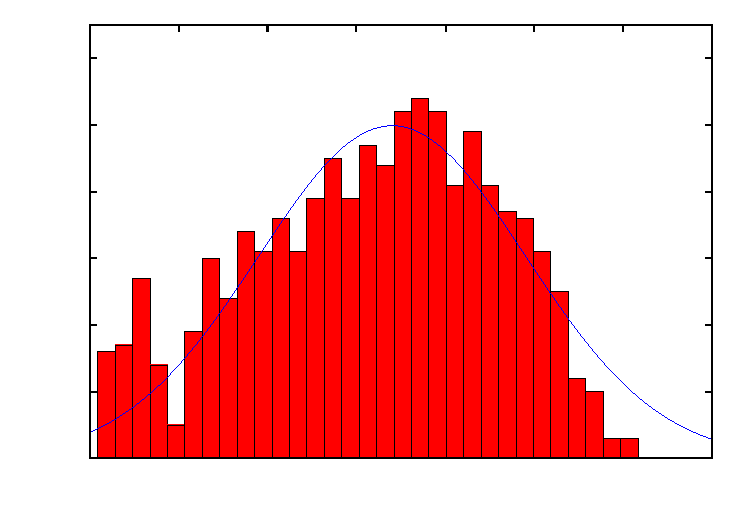
\includegraphics{beatfrequenzen_alt_FOL_histogramm}}%
    \gplfronttext
  \end{picture}%
\endgroup

		}
	}}
	\caption[Beatfrequenzen - altes System mit FOL]{(a) Frequenzverlauf des
	Schwebungssignals der beiden roten FOL-stabilisierten Laser des alten Systems
	über eine Zeit von $30\,$min. (b) zeigt die Frequenzverteilung für die
	komplette Messung (grauer Bereich in (a)).}
	\label{fig:beatfrequenzen_alt_FOL}
\end{figure}
Abbildung
\ref{fig:beatfrequenzen_alt_FOL}\subref{subfig:beatfrequenzen_alt_FOL_drift}
zeigt wie erwartet ein zeitlich stabiles Verhalten ohne Drift. Die
Frequenzverteilung (Abb.
\ref{fig:beatfrequenzen_alt_FOL}\subref{subfig:beatfrequenzen_alt_FOL_histogramm})
ist allerdings wesentlich breiter als im neuen System. Im Histogramm ist eine Asymmetrie am niederfrequenten Rand der
Verteilung zu erkennen. Die dortige Häufung ist damit zu erklären, dass sich das Vorzeichen
der Relativfrequenz im unteren Bereich ab und zu ändern kann. Da die Vorzeichen
aber über Schwebungsfrequenzen nicht unterschieden werden können, entsteht die erwähnte
Asymmetrie, die die Verteilungsbreite fälschlicherweise in geringem Maße
vergrößert. Um keine zu große Verfälschung der Linienbreite zu bekommen, wurde die untere Grenze für die am
Fit beteiligten Werte auf $5\,$MHz gesetzt. Weiterhin hat die Verteilung
untypisch stark abfallende Flanken. Diese könnten durch Ober- bzw.
Untergrenzen der Stabilisisierungsroutine erklärt werden. Aus der Arbeit
\cite{kuschnick:2000:diplomarbeit} geht allerdings nicht hervor, dass eine
derartige Regelbegrenzung implementiert wurde. Allerdings sind trotz
Implementierung im neuen System derartige Regelbeschränkungen im entsprechenden
Frequenzspektrum nicht zu erkennen. Der Gauß-Fit liefert eine Standardabweichung
von $2\sigma_{ges,alt,FOL}=(15,03\pm0,86)\,$MHz, was bei ähnlichen effektiven
Linienbreiten der beiden roten Laser zu
$\sigma_{1,alt,FOL}=\sigma_{2,alt,FOL}=(10,63\pm0,61)\,$MHz führt. Die effektive
Linienbreite ist also mehr als doppelt so groß wie die der kommerziellen Laser
von \textit{Toptica}, was aufgrund der instabileren Bauweise zu erwarten war.
Inwieweit die Stabilisierung darauf Einfluss hat, kann in diesem Fall
nicht herausgefunden werden. Dazu müssten die Laser und die
Stabilisierungstechniken untereinander getauscht und erneute Messungen
durchgeführt werden. Im Rahmen dieser Arbeit wurde dies aber nicht
untersucht. Tabelle \ref{tab:laserstabilitaet} listet noch einmal zum
Vergleich alle wichtigen Größen des Laserverhaltens auf.
\begin{table}[h]
	\small
	%Summe der Breiten muss 0.91 mal \textwidth sein.
	\begin{tabular}{L{0.34\textwidth}|C{0.09\textwidth}C{0.14\textwidth}C{0.13\textwidth}|C{0.08\textwidth}C{0.13\textwidth}|}
	&
		\multicolumn{3}{c|}{\large\textbf{neues System}} &
		\multicolumn{2}{c|}{\large\textbf{altes System}}\\
		\cline{2-6}
		&
		\normalsize\textbf{frei} &
		\normalsize\textbf{\textit{iScan}} &
		\normalsize\textbf{\textit{iScan}+FOL} &
		\normalsize\textbf{frei} &
		\normalsize\textbf{FOL}\\
		\midrule[1px]
		%%%%%%%%%%%%%%%%%%%%%%%%%%%%%%%%%%%%%%%%%%%%%%%%%%%%%%%%%%%%%%%%%%%%%%
%%                                                                  %%
%%  This is a LaTeX2e table fragment exported from Gnumeric.        %%
%%                                                                  %%
%%%%%%%%%%%%%%%%%%%%%%%%%%%%%%%%%%%%%%%%%%%%%%%%%%%%%%%%%%%%%%%%%%%%%%
Drift/2h Laser 1 [Mhz]	&$\approx700$*	&$\approx100$*	&$0$	&-- &--\\
Drift/2h Laser 2 [Mhz]	&$\approx60$*	&$\approx20$*	&$0$	&$\approx300$*	&$0$\\
Drift/2h Laser 3 [Mhz]	&$\approx20$*	&$\approx20$*	&$0$	&--	&--\\
\hline
Jitter Laser 1 [Mhz]	&$<5$	&$<5$	&$<5$	&--	&--\\
Jitter Laser 2 [Mhz]	&$<1,5$	&$<1,5$	&$<1,5$	&$<15$**
&$<15$**\\
Jitter Laser 3 [Mhz]	&$<1,5$	&$<1,5$	&$<1,5$	&--	&--\\
\hline
eff. Linienbreite Laser 1 [Mhz]	&--	&--	&--	&--	&--\\
eff. Linienbreite Laser 2 [Mhz]	&--	&$4,38\pm0,16$	&$3,93\pm0,10$	&--
&$10,63\pm0,61$\\
eff. Linienbreite Laser 3 [Mhz]	&--	&$4,38\pm0,16$	&$3,93\pm0,10$	&--
&$10,63\pm0,61$\\
		\bottomrule[1px]
	\end{tabular}
	\caption[Laserstabilität]{Alle wichtigen Größen zur
	Laserstabilität des neuen und des alten Systems.\\
	* keine Statistik\\
	** kürzere Mittelungszeiten ($\approx85\,$ms), sonst $\approx170\,$ms\\
	"`--"' keine Messungen vorhanden}
	\label{tab:laserstabilitaet}
\end{table}

\section{Linearisierung der
\textit{iScans}}\label{sec:linearisierung_charakterisierung}
Um größere Frequenzverstimmungen mit der neu entwickelten Technik fehlerfrei und
möglichst schnell durchführen zu können, ist es wichtig, dass die
\textit{iScans} linearisiert sind. Die LUTs müssen also derart abgeglichen sein,
dass die internen Frequenzskalen den realen Frequenzabständen entsprechen.
Inwieweit dies realisierbar ist (Abschn. \ref{sec:linearisierungsmessungen}) und was dies
für Frequenzscans bedeutet (Abschn. \ref{sec:frequenz_scans}), soll in
diesem Abschnitt behandelt werden. Exemplarisch sind alle folgenden Messungen
mit dem \textit{DL-Pro} durchgeführt worden.

\subsection{Linearisierungsmessungen}\label{sec:linearisierungsmessungen}
Um eine Aussage über die Linearisierung treffen zu können, wurde das
\textit{iScan} zunächst mit der in Abschn. \ref{sec:linearisierung_iscan}
beschriebenen Routine linearisiert und der Parameter \lstinline|FSR| an den wahren FSR
angepasst. Bei der Linearisierung wurde außerdem
zwischen bereits im Vorhinein korrigiertem \lstinline|FSR| und absichtlich
falsch eingestelltem \lstinline|FSR| unterschieden. Anschließend wurde das
zeitliche Verhalten der Linearität über mehrere Stunden beobachtet.

\subsubsection{Linearisierung mit korrektem
FSR}\label{subsubsec:linearisierung_FSR_okay}
Abbildung \ref{fig:linearisierung_FSR_okay} zeigt den Verlauf des maximal
möglichen Fehlers bei einem Frequenzscan (oben) und die Abweichung des Paramters \lstinline|FSR| vom wahren FSR des \textit{iScans} (unten) in Abhängigkeit vom Iterationsschritt der
Softwareroutine. Dabei liegt \lstinline|FSR| bereits nahe beim wahren FSR und
die LUT wurde vorher zurückgesetzt. Alle Werte sind Absolutbeträge der
Abweichungen.
\begin{figure}[h]
 	\centering
 	\footnotesize
	% GNUPLOT: LaTeX picture with Postscript
\begingroup
  \makeatletter
  \providecommand\color[2][]{%
    \GenericError{(gnuplot) \space\space\space\@spaces}{%
      Package color not loaded in conjunction with
      terminal option `colourtext'%
    }{See the gnuplot documentation for explanation.%
    }{Either use 'blacktext' in gnuplot or load the package
      color.sty in LaTeX.}%
    \renewcommand\color[2][]{}%
  }%
  \providecommand\includegraphics[2][]{%
    \GenericError{(gnuplot) \space\space\space\@spaces}{%
      Package graphicx or graphics not loaded%
    }{See the gnuplot documentation for explanation.%
    }{The gnuplot epslatex terminal needs graphicx.sty or graphics.sty.}%
    \renewcommand\includegraphics[2][]{}%
  }%
  \providecommand\rotatebox[2]{#2}%
  \@ifundefined{ifGPcolor}{%
    \newif\ifGPcolor
    \GPcolortrue
  }{}%
  \@ifundefined{ifGPblacktext}{%
    \newif\ifGPblacktext
    \GPblacktexttrue
  }{}%
  % define a \g@addto@macro without @ in the name:
  \let\gplgaddtomacro\g@addto@macro
  % define empty templates for all commands taking text:
  \gdef\gplbacktext{}%
  \gdef\gplfronttext{}%
  \makeatother
  \ifGPblacktext
    % no textcolor at all
    \def\colorrgb#1{}%
    \def\colorgray#1{}%
  \else
    % gray or color?
    \ifGPcolor
      \def\colorrgb#1{\color[rgb]{#1}}%
      \def\colorgray#1{\color[gray]{#1}}%
      \expandafter\def\csname LTw\endcsname{\color{white}}%
      \expandafter\def\csname LTb\endcsname{\color{black}}%
      \expandafter\def\csname LTa\endcsname{\color{black}}%
      \expandafter\def\csname LT0\endcsname{\color[rgb]{1,0,0}}%
      \expandafter\def\csname LT1\endcsname{\color[rgb]{0,1,0}}%
      \expandafter\def\csname LT2\endcsname{\color[rgb]{0,0,1}}%
      \expandafter\def\csname LT3\endcsname{\color[rgb]{1,0,1}}%
      \expandafter\def\csname LT4\endcsname{\color[rgb]{0,1,1}}%
      \expandafter\def\csname LT5\endcsname{\color[rgb]{1,1,0}}%
      \expandafter\def\csname LT6\endcsname{\color[rgb]{0,0,0}}%
      \expandafter\def\csname LT7\endcsname{\color[rgb]{1,0.3,0}}%
      \expandafter\def\csname LT8\endcsname{\color[rgb]{0.5,0.5,0.5}}%
    \else
      % gray
      \def\colorrgb#1{\color{black}}%
      \def\colorgray#1{\color[gray]{#1}}%
      \expandafter\def\csname LTw\endcsname{\color{white}}%
      \expandafter\def\csname LTb\endcsname{\color{black}}%
      \expandafter\def\csname LTa\endcsname{\color{black}}%
      \expandafter\def\csname LT0\endcsname{\color{black}}%
      \expandafter\def\csname LT1\endcsname{\color{black}}%
      \expandafter\def\csname LT2\endcsname{\color{black}}%
      \expandafter\def\csname LT3\endcsname{\color{black}}%
      \expandafter\def\csname LT4\endcsname{\color{black}}%
      \expandafter\def\csname LT5\endcsname{\color{black}}%
      \expandafter\def\csname LT6\endcsname{\color{black}}%
      \expandafter\def\csname LT7\endcsname{\color{black}}%
      \expandafter\def\csname LT8\endcsname{\color{black}}%
    \fi
  \fi
  \setlength{\unitlength}{0.0500bp}%
  \begin{picture}(7370.00,6802.00)%
    \gplgaddtomacro\gplbacktext{%
      \csname LTb\endcsname%
      \put(1080,3704){\makebox(0,0)[r]{\strut{} 1}}%
      \put(1080,4510){\makebox(0,0)[r]{\strut{} 10}}%
      \put(1080,5316){\makebox(0,0)[r]{\strut{} 100}}%
      \put(1652,3261){\makebox(0,0){\strut{}}}%
      \put(2103,3261){\makebox(0,0){\strut{}}}%
      \put(2555,3261){\makebox(0,0){\strut{}}}%
      \put(3007,3261){\makebox(0,0){\strut{}}}%
      \put(3459,3261){\makebox(0,0){\strut{}}}%
      \put(3910,3261){\makebox(0,0){\strut{}}}%
      \put(4362,3261){\makebox(0,0){\strut{}}}%
      \put(4814,3261){\makebox(0,0){\strut{}}}%
      \put(5266,3261){\makebox(0,0){\strut{}}}%
      \put(5717,3261){\makebox(0,0){\strut{}}}%
      \put(380,4631){\rotatebox{-270}{\makebox(0,0){\strut{}max. Scanfehler [MHz]}}}%
    }%
    \gplgaddtomacro\gplfronttext{%
    }%
    \gplgaddtomacro\gplbacktext{%
      \csname LTb\endcsname%
      \put(1080,1000){\makebox(0,0)[r]{\strut{} 0.1}}%
      \put(1080,2269){\makebox(0,0)[r]{\strut{} 1}}%
      \put(1652,800){\makebox(0,0){\strut{}1}}%
      \put(2103,800){\makebox(0,0){\strut{}2}}%
      \put(2555,800){\makebox(0,0){\strut{}3}}%
      \put(3007,800){\makebox(0,0){\strut{}4}}%
      \put(3459,800){\makebox(0,0){\strut{}5}}%
      \put(3910,800){\makebox(0,0){\strut{}6}}%
      \put(4362,800){\makebox(0,0){\strut{}7}}%
      \put(4814,800){\makebox(0,0){\strut{}8}}%
      \put(5266,800){\makebox(0,0){\strut{}9}}%
      \put(5717,800){\makebox(0,0){\strut{}10}}%
      \put(380,2170){\rotatebox{-270}{\makebox(0,0){\strut{}FSR Fehler [MHz]}}}%
      \put(3684,500){\makebox(0,0){\strut{}Iteration}}%
    }%
    \gplgaddtomacro\gplfronttext{%
    }%
    \gplbacktext
    \put(0,0){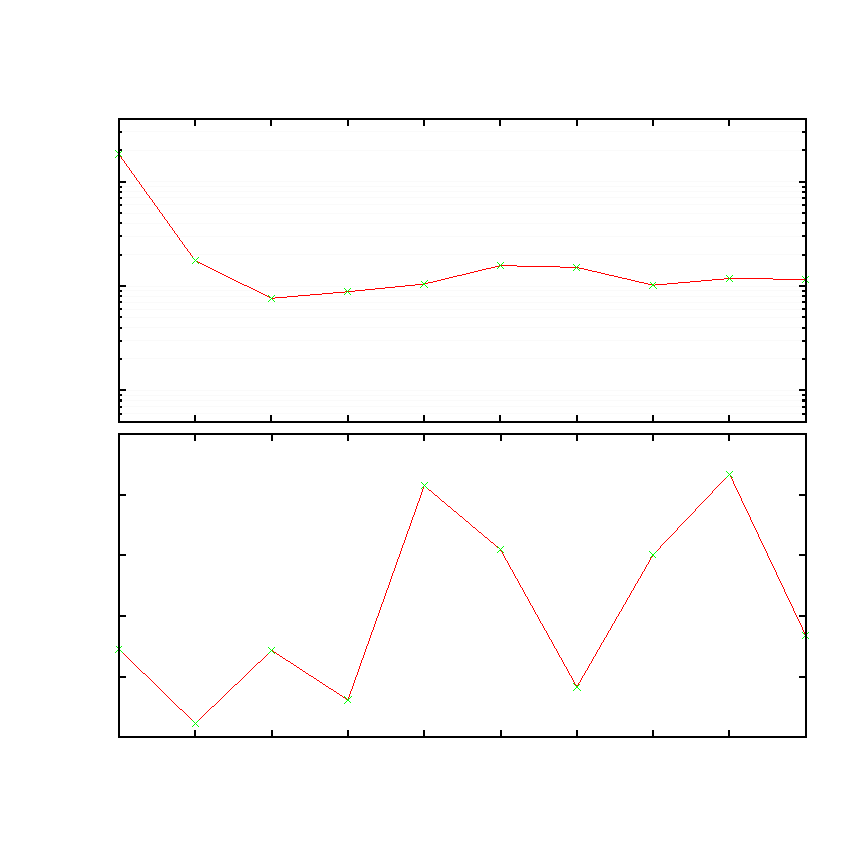
\includegraphics{linearisierung_FSR_okay}}%
    \gplfronttext
  \end{picture}%
\endgroup

	\caption[Linearisierung \textit{iScan}, FSR okay]{Maximaler Scanfehler (oben)
	und Abweichung des Paramters \lstinline|FSR| vom wahren FSR des
	\textit{iScans} (unten) in Abhängigkeit vom Iterationsschritt der
	Softwareroutine, wobei \lstinline|FSR| bereits nahe beim wahren FSR liegt. Alle
	Werte sind Absolutbeträge der Abweichungen.}
	\label{fig:linearisierung_FSR_okay}
\end{figure}
\begin{figure}[h]
 	\centering
 	\footnotesize
	% GNUPLOT: LaTeX picture with Postscript
\begingroup
  \makeatletter
  \providecommand\color[2][]{%
    \GenericError{(gnuplot) \space\space\space\@spaces}{%
      Package color not loaded in conjunction with
      terminal option `colourtext'%
    }{See the gnuplot documentation for explanation.%
    }{Either use 'blacktext' in gnuplot or load the package
      color.sty in LaTeX.}%
    \renewcommand\color[2][]{}%
  }%
  \providecommand\includegraphics[2][]{%
    \GenericError{(gnuplot) \space\space\space\@spaces}{%
      Package graphicx or graphics not loaded%
    }{See the gnuplot documentation for explanation.%
    }{The gnuplot epslatex terminal needs graphicx.sty or graphics.sty.}%
    \renewcommand\includegraphics[2][]{}%
  }%
  \providecommand\rotatebox[2]{#2}%
  \@ifundefined{ifGPcolor}{%
    \newif\ifGPcolor
    \GPcolortrue
  }{}%
  \@ifundefined{ifGPblacktext}{%
    \newif\ifGPblacktext
    \GPblacktexttrue
  }{}%
  % define a \g@addto@macro without @ in the name:
  \let\gplgaddtomacro\g@addto@macro
  % define empty templates for all commands taking text:
  \gdef\gplbacktext{}%
  \gdef\gplfronttext{}%
  \makeatother
  \ifGPblacktext
    % no textcolor at all
    \def\colorrgb#1{}%
    \def\colorgray#1{}%
  \else
    % gray or color?
    \ifGPcolor
      \def\colorrgb#1{\color[rgb]{#1}}%
      \def\colorgray#1{\color[gray]{#1}}%
      \expandafter\def\csname LTw\endcsname{\color{white}}%
      \expandafter\def\csname LTb\endcsname{\color{black}}%
      \expandafter\def\csname LTa\endcsname{\color{black}}%
      \expandafter\def\csname LT0\endcsname{\color[rgb]{1,0,0}}%
      \expandafter\def\csname LT1\endcsname{\color[rgb]{0,1,0}}%
      \expandafter\def\csname LT2\endcsname{\color[rgb]{0,0,1}}%
      \expandafter\def\csname LT3\endcsname{\color[rgb]{1,0,1}}%
      \expandafter\def\csname LT4\endcsname{\color[rgb]{0,1,1}}%
      \expandafter\def\csname LT5\endcsname{\color[rgb]{1,1,0}}%
      \expandafter\def\csname LT6\endcsname{\color[rgb]{0,0,0}}%
      \expandafter\def\csname LT7\endcsname{\color[rgb]{1,0.3,0}}%
      \expandafter\def\csname LT8\endcsname{\color[rgb]{0.5,0.5,0.5}}%
    \else
      % gray
      \def\colorrgb#1{\color{black}}%
      \def\colorgray#1{\color[gray]{#1}}%
      \expandafter\def\csname LTw\endcsname{\color{white}}%
      \expandafter\def\csname LTb\endcsname{\color{black}}%
      \expandafter\def\csname LTa\endcsname{\color{black}}%
      \expandafter\def\csname LT0\endcsname{\color{black}}%
      \expandafter\def\csname LT1\endcsname{\color{black}}%
      \expandafter\def\csname LT2\endcsname{\color{black}}%
      \expandafter\def\csname LT3\endcsname{\color{black}}%
      \expandafter\def\csname LT4\endcsname{\color{black}}%
      \expandafter\def\csname LT5\endcsname{\color{black}}%
      \expandafter\def\csname LT6\endcsname{\color{black}}%
      \expandafter\def\csname LT7\endcsname{\color{black}}%
      \expandafter\def\csname LT8\endcsname{\color{black}}%
    \fi
  \fi
  \setlength{\unitlength}{0.0500bp}%
  \begin{picture}(7370.00,6802.00)%
    \gplgaddtomacro\gplbacktext{%
      \csname LTb\endcsname%
      \put(1080,3704){\makebox(0,0)[r]{\strut{} 1}}%
      \put(1080,4510){\makebox(0,0)[r]{\strut{} 10}}%
      \put(1080,5316){\makebox(0,0)[r]{\strut{} 100}}%
      \put(2028,3261){\makebox(0,0){\strut{}}}%
      \put(2856,3261){\makebox(0,0){\strut{}}}%
      \put(3684,3261){\makebox(0,0){\strut{}}}%
      \put(4513,3261){\makebox(0,0){\strut{}}}%
      \put(5341,3261){\makebox(0,0){\strut{}}}%
      \put(380,4631){\rotatebox{-270}{\makebox(0,0){\strut{}max. Scanfehler [MHz]}}}%
    }%
    \gplgaddtomacro\gplfronttext{%
    }%
    \gplgaddtomacro\gplbacktext{%
      \csname LTb\endcsname%
      \put(1080,1000){\makebox(0,0)[r]{\strut{} 0.01}}%
      \put(1080,1523){\makebox(0,0)[r]{\strut{} 0.1}}%
      \put(1080,2046){\makebox(0,0)[r]{\strut{} 1}}%
      \put(1080,2569){\makebox(0,0)[r]{\strut{} 10}}%
      \put(1080,3092){\makebox(0,0)[r]{\strut{} 100}}%
      \put(2028,800){\makebox(0,0){\strut{}1}}%
      \put(2856,800){\makebox(0,0){\strut{}2}}%
      \put(3684,800){\makebox(0,0){\strut{}3}}%
      \put(4513,800){\makebox(0,0){\strut{}4}}%
      \put(5341,800){\makebox(0,0){\strut{}5}}%
      \put(440,2170){\rotatebox{-270}{\makebox(0,0){\strut{}FSR Fehler [MHz]}}}%
      \put(3684,500){\makebox(0,0){\strut{}Iteration}}%
    }%
    \gplgaddtomacro\gplfronttext{%
    }%
    \gplbacktext
    \put(0,0){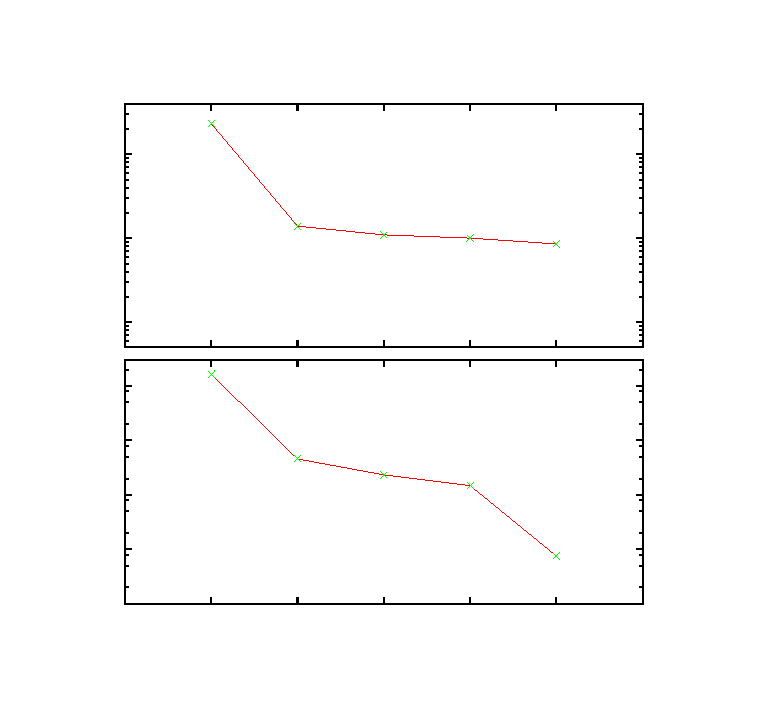
\includegraphics{linearisierung_FSR_korr}}%
    \gplfronttext
  \end{picture}%
\endgroup

	\caption[Linearisierung \textit{iScan}, FSR korrigiert (1)]{Maximaler
	Scanfehler (oben) und Abweichung des Paramters \lstinline|FSR| vom wahren
	FSR des \textit{iScans} (unten) in Abhängigkeit vom Iterationsschritt der
	Softwareroutine, wobei \lstinline|FSR| zuvor absichtlich auf den falschen FSR
	von $8000\,$MHz eingestellt wurde. Alle Werte sind Absolutbeträge der Abweichungen.}
	\label{fig:linearisierung_FSR_korr}
\end{figure}
Der maximal mögliche Scanfehler reduziert sich von
ca. $184\,$MHz auf ca. $8\,$MHz innerhalb von zwei Iterationsschritten. Danach
fluktuiert der Wert in der Größenordnung von $10\,$MHz. Ein kleinerer Wert ist
anscheinend mit dem momentan verwendeten Algorithmus nicht realisierbar. Der
Parameter \lstinline|FSR|, der ggf. nachkorrigiert wird, weicht
während der Linearisierungsphase um maximal ca. $4\,$MHz vom wahren Wert ab und
wurde am Ende der Routine zu $8160\,$MHz bestimmt\footnote{Das \textit{iScan}
hat eine Auflösung von $1\,$MHz, deshalb die Ganzzahlrundung.}. Diese Werte sind
für die korrekte Funktionsweise der Laserkontrolle ausreichend. Auch schnelle Verstimmungen mit großen
Relativfrequenzen sollten damit möglich sein.

\subsubsection{Linearisierung mit anfangs falschem
FSR}\label{subsubsec:linearisierung_FSR_korr}
Eine weitere Linearisierung wurde bei vorher absichtlich auf einen fehlerhaften
Wert von $8000\,$MHz eingestellten \lstinline|FSR| durchgeführt und ist in
Abb. \ref{fig:linearisierung_FSR_korr} dargestellt. Auch hier pendelt sich der
maximal mögliche Scanfehler innerhalb von zwei Iterationen von anfangs ca.
$184\,$MHz auf einen Wert um $10\,$MHz ein. Nahezu synchron wird der zuvor um
$164\,$MHz falsch eingestellte Parameter \lstinline|FSR| an den wahren Wert
mit einer finalen Abweichung von $<1\,$MHz herangeführt. Die Abweichung
der \textit{iScan}-Frequenzskala von den wahren Werten ist für jeden
Iterationsschritt dieser Messung exemplarisch in Anh.
\ref{anh:sec:linearisierung} dargestellt. Bei allen Messungen und Korrekturen
muss allerdings beachtet werden, dass aufgrund der begrenzten Anzahl von
Messpunkten (n=$\lfloor\nicefrac{\text{FSR}_{iScan}}{\text{FSR}_{FPI}}\rfloor+2$) die
berechneten Abweichungen von der Linearität mit dem wahren \textit{iScan}-FSR
korreliert sein können, was die Mess- und Korrekturwerte verfälschen kann. Es
zeigt sich jedoch, dass trotz dieser Tatsache bereits nach zweimaligem
Durchlaufen der Linearisierungsroutine akzeptable Ausgangswerte zur weiteren
Stabilisierungs- und Frequenzverstimmungstechnik erreicht werden können, was
innerhalb weniger Minuten mit geringem Aufwand erledigt werden kann.

\subsubsection{Zeitliches Verhalten
der Linearität}\label{subsubsec:linearitaet_verlauf}
Um zu erfahren, wie
sich die Abweichungen von den Idealwerten zeitlich verhalten, wurden diese über
mehrere Stunden ohne Korrekturmaßnahmen beobachtet. Es wurde ca. alle $5\,$min ein Fringepattern aufgenommen und analysiert. Die Messung wurde unmittelbar nach Beendigung der Linearisierung aus Abb.
\ref{fig:linearisierung_FSR_korr} gestartet.
Die Ergebnisse sind analog zu den vorherigen Plots in Abb.
\ref{fig:linearitaet_verlauf} dargestellt.
\begin{figure}
	 	\centering
	 	\footnotesize
		% GNUPLOT: LaTeX picture with Postscript
\begingroup
  \makeatletter
  \providecommand\color[2][]{%
    \GenericError{(gnuplot) \space\space\space\@spaces}{%
      Package color not loaded in conjunction with
      terminal option `colourtext'%
    }{See the gnuplot documentation for explanation.%
    }{Either use 'blacktext' in gnuplot or load the package
      color.sty in LaTeX.}%
    \renewcommand\color[2][]{}%
  }%
  \providecommand\includegraphics[2][]{%
    \GenericError{(gnuplot) \space\space\space\@spaces}{%
      Package graphicx or graphics not loaded%
    }{See the gnuplot documentation for explanation.%
    }{The gnuplot epslatex terminal needs graphicx.sty or graphics.sty.}%
    \renewcommand\includegraphics[2][]{}%
  }%
  \providecommand\rotatebox[2]{#2}%
  \@ifundefined{ifGPcolor}{%
    \newif\ifGPcolor
    \GPcolortrue
  }{}%
  \@ifundefined{ifGPblacktext}{%
    \newif\ifGPblacktext
    \GPblacktexttrue
  }{}%
  % define a \g@addto@macro without @ in the name:
  \let\gplgaddtomacro\g@addto@macro
  % define empty templates for all commands taking text:
  \gdef\gplbacktext{}%
  \gdef\gplfronttext{}%
  \makeatother
  \ifGPblacktext
    % no textcolor at all
    \def\colorrgb#1{}%
    \def\colorgray#1{}%
  \else
    % gray or color?
    \ifGPcolor
      \def\colorrgb#1{\color[rgb]{#1}}%
      \def\colorgray#1{\color[gray]{#1}}%
      \expandafter\def\csname LTw\endcsname{\color{white}}%
      \expandafter\def\csname LTb\endcsname{\color{black}}%
      \expandafter\def\csname LTa\endcsname{\color{black}}%
      \expandafter\def\csname LT0\endcsname{\color[rgb]{1,0,0}}%
      \expandafter\def\csname LT1\endcsname{\color[rgb]{0,1,0}}%
      \expandafter\def\csname LT2\endcsname{\color[rgb]{0,0,1}}%
      \expandafter\def\csname LT3\endcsname{\color[rgb]{1,0,1}}%
      \expandafter\def\csname LT4\endcsname{\color[rgb]{0,1,1}}%
      \expandafter\def\csname LT5\endcsname{\color[rgb]{1,1,0}}%
      \expandafter\def\csname LT6\endcsname{\color[rgb]{0,0,0}}%
      \expandafter\def\csname LT7\endcsname{\color[rgb]{1,0.3,0}}%
      \expandafter\def\csname LT8\endcsname{\color[rgb]{0.5,0.5,0.5}}%
    \else
      % gray
      \def\colorrgb#1{\color{black}}%
      \def\colorgray#1{\color[gray]{#1}}%
      \expandafter\def\csname LTw\endcsname{\color{white}}%
      \expandafter\def\csname LTb\endcsname{\color{black}}%
      \expandafter\def\csname LTa\endcsname{\color{black}}%
      \expandafter\def\csname LT0\endcsname{\color{black}}%
      \expandafter\def\csname LT1\endcsname{\color{black}}%
      \expandafter\def\csname LT2\endcsname{\color{black}}%
      \expandafter\def\csname LT3\endcsname{\color{black}}%
      \expandafter\def\csname LT4\endcsname{\color{black}}%
      \expandafter\def\csname LT5\endcsname{\color{black}}%
      \expandafter\def\csname LT6\endcsname{\color{black}}%
      \expandafter\def\csname LT7\endcsname{\color{black}}%
      \expandafter\def\csname LT8\endcsname{\color{black}}%
    \fi
  \fi
  \setlength{\unitlength}{0.0500bp}%
  \begin{picture}(7370.00,9636.00)%
    \gplgaddtomacro\gplbacktext{%
      \csname LTb\endcsname%
      \put(-120,7050){\makebox(0,0)[r]{\strut{}-60}}%
      \put(-120,7620){\makebox(0,0)[r]{\strut{}-40}}%
      \put(-120,8190){\makebox(0,0)[r]{\strut{}-20}}%
      \put(-120,8760){\makebox(0,0)[r]{\strut{} 0}}%
      \put(-120,9330){\makebox(0,0)[r]{\strut{} 20}}%
      \put(245,6565){\makebox(0,0){\strut{} 0}}%
      \put(736,6565){\makebox(0,0){\strut{} 2}}%
      \put(1227,6565){\makebox(0,0){\strut{} 4}}%
      \put(1717,6565){\makebox(0,0){\strut{} 6}}%
      \put(2208,6565){\makebox(0,0){\strut{} 8}}%
      \put(-616,8190){\rotatebox{-270}{\makebox(0,0){\strut{}Abweichung [MHz]}}}%
      \put(1226,6365){\makebox(0,0){\strut{}Scan Position [GHz]}}%
      \put(1104,9330){\makebox(0,0)[l]{\strut{}A}}%
      \put(245,7193){\makebox(0,0)[l]{\strut{}\tiny{max. m"ogl. Abweichung: $11.2$ MHz}}}%
    }%
    \gplgaddtomacro\gplfronttext{%
      \csname LTb\endcsname%
      \put(1670,7805){\makebox(0,0)[r]{\strut{}\tiny{zw. Fringes [MHz]}}}%
      \csname LTb\endcsname%
      \put(1670,7605){\makebox(0,0)[r]{\strut{}\tiny{absolut [MHz]}}}%
    }%
    \gplgaddtomacro\gplbacktext{%
      \csname LTb\endcsname%
      \put(2334,7050){\makebox(0,0)[r]{\strut{}}}%
      \put(2334,7620){\makebox(0,0)[r]{\strut{}}}%
      \put(2334,8190){\makebox(0,0)[r]{\strut{}}}%
      \put(2334,8760){\makebox(0,0)[r]{\strut{}}}%
      \put(2334,9330){\makebox(0,0)[r]{\strut{}}}%
      \put(2699,6565){\makebox(0,0){\strut{} 0}}%
      \put(3190,6565){\makebox(0,0){\strut{} 2}}%
      \put(3681,6565){\makebox(0,0){\strut{} 4}}%
      \put(4171,6565){\makebox(0,0){\strut{} 6}}%
      \put(4662,6565){\makebox(0,0){\strut{} 8}}%
      \put(3680,6365){\makebox(0,0){\strut{}Scan Position [GHz]}}%
      \put(3558,9330){\makebox(0,0)[l]{\strut{}B}}%
      \put(2699,7193){\makebox(0,0)[l]{\strut{}\tiny{max. m"ogl. Abweichung: $54.2$ MHz}}}%
    }%
    \gplgaddtomacro\gplfronttext{%
    }%
    \gplgaddtomacro\gplbacktext{%
      \csname LTb\endcsname%
      \put(4788,7050){\makebox(0,0)[r]{\strut{}}}%
      \put(4788,7620){\makebox(0,0)[r]{\strut{}}}%
      \put(4788,8190){\makebox(0,0)[r]{\strut{}}}%
      \put(4788,8760){\makebox(0,0)[r]{\strut{}}}%
      \put(4788,9330){\makebox(0,0)[r]{\strut{}}}%
      \put(5152,6565){\makebox(0,0){\strut{} 0}}%
      \put(5640,6565){\makebox(0,0){\strut{} 2}}%
      \put(6128,6565){\makebox(0,0){\strut{} 4}}%
      \put(6617,6565){\makebox(0,0){\strut{} 6}}%
      \put(7105,6565){\makebox(0,0){\strut{} 8}}%
      \put(6128,6365){\makebox(0,0){\strut{}Scan Position [GHz]}}%
      \put(6006,9330){\makebox(0,0)[l]{\strut{}C}}%
      \put(5152,7193){\makebox(0,0)[l]{\strut{}\tiny{max. m"ogl. Abweichung: $79.8$ MHz}}}%
    }%
    \gplgaddtomacro\gplfronttext{%
    }%
    \gplgaddtomacro\gplbacktext{%
      \csname LTb\endcsname%
      \put(-120,3214){\makebox(0,0)[r]{\strut{}10}}%
      \put(-120,3519){\makebox(0,0)[r]{\strut{}20}}%
      \put(-120,3823){\makebox(0,0)[r]{\strut{}30}}%
      \put(-120,4128){\makebox(0,0)[r]{\strut{}40}}%
      \put(-120,4432){\makebox(0,0)[r]{\strut{}50}}%
      \put(-120,4736){\makebox(0,0)[r]{\strut{}60}}%
      \put(-120,5041){\makebox(0,0)[r]{\strut{}70}}%
      \put(-120,5345){\makebox(0,0)[r]{\strut{}80}}%
      \put(-120,5650){\makebox(0,0)[r]{\strut{}90}}%
      \put(669,2710){\makebox(0,0){\strut{}}}%
      \put(1337,2710){\makebox(0,0){\strut{}}}%
      \put(2006,2710){\makebox(0,0){\strut{}}}%
      \put(2675,2710){\makebox(0,0){\strut{}}}%
      \put(3344,2710){\makebox(0,0){\strut{}}}%
      \put(4012,2710){\makebox(0,0){\strut{}}}%
      \put(4681,2710){\makebox(0,0){\strut{}}}%
      \put(5350,2710){\makebox(0,0){\strut{}}}%
      \put(6019,2710){\makebox(0,0){\strut{}}}%
      \put(6687,2710){\makebox(0,0){\strut{}}}%
      \put(-580,4432){\rotatebox{-270}{\makebox(0,0){\strut{}max. Scanfehler [MHz]}}}%
      \put(602,3915){\makebox(0,0)[l]{\strut{}A}}%
      \put(2461,5132){\makebox(0,0)[l]{\strut{}B}}%
      \put(4053,5558){\makebox(0,0)[l]{\strut{}C}}%
    }%
    \gplgaddtomacro\gplfronttext{%
    }%
    \gplgaddtomacro\gplbacktext{%
      \csname LTb\endcsname%
      \put(-120,1234){\makebox(0,0)[r]{\strut{}-6}}%
      \put(-120,1468){\makebox(0,0)[r]{\strut{}-4}}%
      \put(-120,1702){\makebox(0,0)[r]{\strut{}-2}}%
      \put(-120,1936){\makebox(0,0)[r]{\strut{}0}}%
      \put(-120,2169){\makebox(0,0)[r]{\strut{}2}}%
      \put(-120,2403){\makebox(0,0)[r]{\strut{}4}}%
      \put(-120,2637){\makebox(0,0)[r]{\strut{}6}}%
      \put(669,800){\makebox(0,0){\strut{}0}}%
      \put(1337,800){\makebox(0,0){\strut{}30}}%
      \put(2006,800){\makebox(0,0){\strut{}60}}%
      \put(2675,800){\makebox(0,0){\strut{}90}}%
      \put(3344,800){\makebox(0,0){\strut{}120}}%
      \put(4012,800){\makebox(0,0){\strut{}150}}%
      \put(4681,800){\makebox(0,0){\strut{}180}}%
      \put(5350,800){\makebox(0,0){\strut{}210}}%
      \put(6019,800){\makebox(0,0){\strut{}240}}%
      \put(6687,800){\makebox(0,0){\strut{}270}}%
      \put(-580,1935){\rotatebox{-270}{\makebox(0,0){\strut{}FSR-Fehler [MHz]}}}%
      \put(3678,500){\makebox(0,0){\strut{}Zeit [min]}}%
    }%
    \gplgaddtomacro\gplfronttext{%
    }%
    \gplbacktext
    \put(0,0){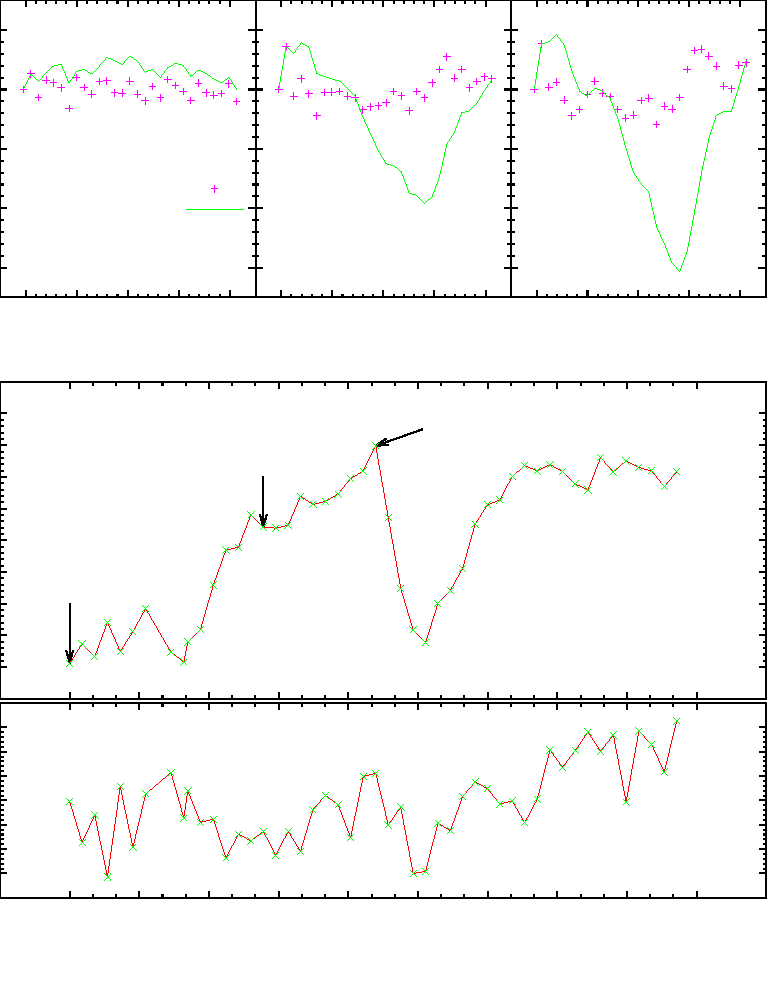
\includegraphics{linearitaet_verlauf}}%
    \gplfronttext
  \end{picture}%
\endgroup

		\caption[Linearitaet \textit{iScan}, zeitlicher Verlauf]{Auswahl von drei
		Fringepatternanalysen (oben), zeitlicher Verlauf des maximalen Scanfehler
		(mitte) und der Abweichung des Paramters \lstinline|FSR| vom wahren FSR des
		\textit{iScans} (unten). Die Messung wurde unmittelbar nach Beendigung der
		Linearisierung aus Abb. \ref{fig:linearisierung_FSR_korr} gestartet.}
		\label{fig:linearitaet_verlauf}
\end{figure}
Zu verschiedenen Zeiten sind zusätzlich oben in Abb.
\ref{fig:linearitaet_verlauf} Linearitätsabweichungs-Plots der mit Pfeilen
zugeordneten Messpunkte dargestellt. Dabei sind die maximal möglichen Scanfehler
die Differenzen zwischen Maxima und Minima der grünen Kurven.\par
Der FSR des
\textit{iScans} ist offensichtlich eine unkritische und gegen Drifts
resistente Größe. Dies entspricht den Erwartungen, da sich die Eigenschaften des
\textit{iScan}-Etalons verschwindend gering mit Störparametern wie der
Temperatur ändern. Der FSR schwankt scheinbar innerhalb von $4,5\,$h um maximal
$\pm6\,$MHz, wobei es sich hierbei wie schon oben erwähnt um eine ungenaue
Angabe handelt, da dieser Messwert aufgrund der Messtechnik in der Größenordnung von mehreren MHz mit der Linearität des \textit{iScans} korreliert sein kann. Der nur qualitativ abschätzbare Fehler bei der Berechnung des FSR-Fehlers liegt vermutlich in der Größenordnung seiner
Fluktuation. Für die bei den Messungen benötigte Präzision genügt es daher
einmal täglich den Parameter \lstinline|FSR| aufgund geringfügiger Drifts zu korrigieren.\par
Anders verhält es sich mit der Linearität des \textit{iScans}.
Der maximal mögliche Fehler ist starken Drifts unterworfen und bewegt sich
innerhalb von $4,5\,$h zwischen $10$ und $80\,$MHz. Dabei handelt es sich
nicht um eine konstante Drift, sodern um unterschiedlich starke Fluktuationen,
die den Anschein erwecken, dass Temperaturänderungen hier eine starke Rolle
spielen. Die wahrscheinlichste Fehlerquelle ist die extrem sensitive
Strahleinkopplung in die \textit{iScans}, die durch Hebelwirkung der Spiegel
schon bei kleinen Temperaturänderungen signifikante Linearitätsänderungen hevorruft. Auch zu
erkennen ist, dass ab einem bestimmten Grad der räumlichen Verstimmung die
Sensitivität abnimmt und nur noch geringe Linearitätsänderungen möglich sind. Um
dies genauer zu prüfen müssen in Zukunft weitere länger angelegte Messungen
durchgeführt werden, wobei auch eine Temperaturkorrelation nachzuprüfen ist.
Kann diese bestätigt werden, wäre es sinnvoll, eine Laser$\rightarrow$\textit{iScan}-Faserkopplung nachzurüsten.\par
Mit dem momentanen Aufbau ist es ratsam täglich vor Messbeginn eine
Linearisierung für jedes \textit{iScan}-System durchzuführen. Für die
Stabilisierungs- und Scanroutine ist die in diesem Experiment gemessene maximale Abweichung
allerdings unkritisch. Negative Auswirkungen hat dies nur auf die Geschwindigkeit der
Regelung, wodurch die Messphasen von Isotopenverhältnismessungen erheblich
verlängert werden. Im nächsten Abschnitt soll nun quantitativ überprüft werden,
inwieweit das System bei (nicht-)Linearität den Performanceansprüchen, die an
die Frequenzverstimmung gestellt werden, gerecht wird.

\subsection{Frequenzscans}\label{sec:frequenz_scans}
In diesem Abschnitt werden die Auswirkungen der im vorherigen Abschnitt
behandelten \textit{iScan}-Nichtlinearitäten auf große Frequenzverstimmungen
von mehreren GHz, wie sie bei Isotopenverhältnismessungen üblich sind,
untersucht. Dabei wird insbesondere auf die Geschwindigkeit der in Abschn.
\ref{sec:stabilisierung_frequenzverstimmungs-strategie}
behandelten Verstimmungsroutine und die Dauer der Nachreglung durch das FOL
eingegangen. Zunächst sollen die Ergebnisse für die Messung mit nichtlinearem
\textit{iScan} (LUT zurückgesetzt) diskutiert werden. Anschließend werden die
Ergebnisse mit denen einer Messung mit linearisierten \textit{iScans}
verglichen. Alle Messungen wurden exemplarisch mit dem \textit{DL-Pro}
durchgeführt.

\subsubsection{Frequenzscans mit nichtlinearem
\textit{iScan}}\label{subsubsec:frequenz_scans_nichtlineares_iScan}
Abbildung \ref{fig:laserscan_LUT-reset} zeigt den zeitlichen Verlauf der
Ist- und Soll-Relativfrequenzen des Lasers, wobei regelmäßig eine neue
Sollfrequenz (mehrere GHz verstimmt zur vorherigen) vorgegeben
wurde. In Abb. \ref{fig:laserscan_LUT-reset_zoom} sind die einzelnen
Frequenzverstimmungsschritte vergrößert dargestellt. Die Frequenzachse wurde
dabei aufgeteilt, um den unwichtigen Bereich zwischend den
Soll-Relativfrequenzen auszusparen.
\begin{figure}[h]
	 	\centering
	 	\footnotesize
		% GNUPLOT: LaTeX picture with Postscript
\begingroup
  \makeatletter
  \providecommand\color[2][]{%
    \GenericError{(gnuplot) \space\space\space\@spaces}{%
      Package color not loaded in conjunction with
      terminal option `colourtext'%
    }{See the gnuplot documentation for explanation.%
    }{Either use 'blacktext' in gnuplot or load the package
      color.sty in LaTeX.}%
    \renewcommand\color[2][]{}%
  }%
  \providecommand\includegraphics[2][]{%
    \GenericError{(gnuplot) \space\space\space\@spaces}{%
      Package graphicx or graphics not loaded%
    }{See the gnuplot documentation for explanation.%
    }{The gnuplot epslatex terminal needs graphicx.sty or graphics.sty.}%
    \renewcommand\includegraphics[2][]{}%
  }%
  \providecommand\rotatebox[2]{#2}%
  \@ifundefined{ifGPcolor}{%
    \newif\ifGPcolor
    \GPcolortrue
  }{}%
  \@ifundefined{ifGPblacktext}{%
    \newif\ifGPblacktext
    \GPblacktexttrue
  }{}%
  % define a \g@addto@macro without @ in the name:
  \let\gplgaddtomacro\g@addto@macro
  % define empty templates for all commands taking text:
  \gdef\gplbacktext{}%
  \gdef\gplfronttext{}%
  \makeatother
  \ifGPblacktext
    % no textcolor at all
    \def\colorrgb#1{}%
    \def\colorgray#1{}%
  \else
    % gray or color?
    \ifGPcolor
      \def\colorrgb#1{\color[rgb]{#1}}%
      \def\colorgray#1{\color[gray]{#1}}%
      \expandafter\def\csname LTw\endcsname{\color{white}}%
      \expandafter\def\csname LTb\endcsname{\color{black}}%
      \expandafter\def\csname LTa\endcsname{\color{black}}%
      \expandafter\def\csname LT0\endcsname{\color[rgb]{1,0,0}}%
      \expandafter\def\csname LT1\endcsname{\color[rgb]{0,1,0}}%
      \expandafter\def\csname LT2\endcsname{\color[rgb]{0,0,1}}%
      \expandafter\def\csname LT3\endcsname{\color[rgb]{1,0,1}}%
      \expandafter\def\csname LT4\endcsname{\color[rgb]{0,1,1}}%
      \expandafter\def\csname LT5\endcsname{\color[rgb]{1,1,0}}%
      \expandafter\def\csname LT6\endcsname{\color[rgb]{0,0,0}}%
      \expandafter\def\csname LT7\endcsname{\color[rgb]{1,0.3,0}}%
      \expandafter\def\csname LT8\endcsname{\color[rgb]{0.5,0.5,0.5}}%
    \else
      % gray
      \def\colorrgb#1{\color{black}}%
      \def\colorgray#1{\color[gray]{#1}}%
      \expandafter\def\csname LTw\endcsname{\color{white}}%
      \expandafter\def\csname LTb\endcsname{\color{black}}%
      \expandafter\def\csname LTa\endcsname{\color{black}}%
      \expandafter\def\csname LT0\endcsname{\color{black}}%
      \expandafter\def\csname LT1\endcsname{\color{black}}%
      \expandafter\def\csname LT2\endcsname{\color{black}}%
      \expandafter\def\csname LT3\endcsname{\color{black}}%
      \expandafter\def\csname LT4\endcsname{\color{black}}%
      \expandafter\def\csname LT5\endcsname{\color{black}}%
      \expandafter\def\csname LT6\endcsname{\color{black}}%
      \expandafter\def\csname LT7\endcsname{\color{black}}%
      \expandafter\def\csname LT8\endcsname{\color{black}}%
    \fi
  \fi
  \setlength{\unitlength}{0.0500bp}%
  \begin{picture}(7370.00,3968.00)%
    \gplgaddtomacro\gplbacktext{%
      \csname LTb\endcsname%
      \put(980,640){\makebox(0,0)[r]{\strut{}-4000}}%
      \put(980,1026){\makebox(0,0)[r]{\strut{}-3000}}%
      \put(980,1412){\makebox(0,0)[r]{\strut{}-2000}}%
      \put(980,1798){\makebox(0,0)[r]{\strut{}-1000}}%
      \put(980,2184){\makebox(0,0)[r]{\strut{} 0}}%
      \put(980,2569){\makebox(0,0)[r]{\strut{} 1000}}%
      \put(980,2955){\makebox(0,0)[r]{\strut{} 2000}}%
      \put(980,3341){\makebox(0,0)[r]{\strut{} 3000}}%
      \put(980,3727){\makebox(0,0)[r]{\strut{} 4000}}%
      \put(1100,440){\makebox(0,0){\strut{} 0}}%
      \put(2085,440){\makebox(0,0){\strut{} 10}}%
      \put(3070,440){\makebox(0,0){\strut{} 20}}%
      \put(4055,440){\makebox(0,0){\strut{} 30}}%
      \put(5039,440){\makebox(0,0){\strut{} 40}}%
      \put(6024,440){\makebox(0,0){\strut{} 50}}%
      \put(7009,440){\makebox(0,0){\strut{} 60}}%
      \put(160,2183){\rotatebox{-270}{\makebox(0,0){\strut{}Relativfrequenz [MHz]}}}%
      \put(4054,140){\makebox(0,0){\strut{}Zeit [s]}}%
    }%
    \gplgaddtomacro\gplfronttext{%
      \csname LTb\endcsname%
      \put(6106,3564){\makebox(0,0)[r]{\strut{}Soll-Frequenz}}%
      \csname LTb\endcsname%
      \put(6106,3364){\makebox(0,0)[r]{\strut{}Ist-Frequenz}}%
    }%
    \gplbacktext
    \put(0,0){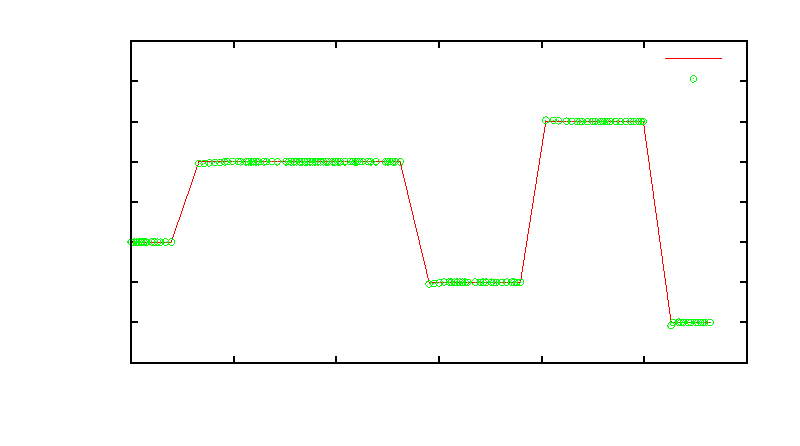
\includegraphics{laserscan_LUT-reset}}%
    \gplfronttext
  \end{picture}%
\endgroup

		\caption[Frequenzscan, nichtlineares \textit{iScan}]{Mehrere
		Frequenzverstimmungen mithilfe der neu entwickelten Software und nichtlinearem
		\textit{iScan}.}
		\label{fig:laserscan_LUT-reset}
\end{figure}
\begin{figure}[hp]
 	\centering
 	\footnotesize
 	\fbox{\parbox{\dimexpr \linewidth - 2\fboxrule - 2\fboxsep}{
 	\subfloat[$-1000\,$GHz $\rightarrow$ $1000\,$GHz]{
		\label{subfig:laserscan_LUT-reset_zoom_01}
		% GNUPLOT: LaTeX picture with Postscript
\begingroup
  \makeatletter
  \providecommand\color[2][]{%
    \GenericError{(gnuplot) \space\space\space\@spaces}{%
      Package color not loaded in conjunction with
      terminal option `colourtext'%
    }{See the gnuplot documentation for explanation.%
    }{Either use 'blacktext' in gnuplot or load the package
      color.sty in LaTeX.}%
    \renewcommand\color[2][]{}%
  }%
  \providecommand\includegraphics[2][]{%
    \GenericError{(gnuplot) \space\space\space\@spaces}{%
      Package graphicx or graphics not loaded%
    }{See the gnuplot documentation for explanation.%
    }{The gnuplot epslatex terminal needs graphicx.sty or graphics.sty.}%
    \renewcommand\includegraphics[2][]{}%
  }%
  \providecommand\rotatebox[2]{#2}%
  \@ifundefined{ifGPcolor}{%
    \newif\ifGPcolor
    \GPcolortrue
  }{}%
  \@ifundefined{ifGPblacktext}{%
    \newif\ifGPblacktext
    \GPblacktexttrue
  }{}%
  % define a \g@addto@macro without @ in the name:
  \let\gplgaddtomacro\g@addto@macro
  % define empty templates for all commands taking text:
  \gdef\gplbacktext{}%
  \gdef\gplfronttext{}%
  \makeatother
  \ifGPblacktext
    % no textcolor at all
    \def\colorrgb#1{}%
    \def\colorgray#1{}%
  \else
    % gray or color?
    \ifGPcolor
      \def\colorrgb#1{\color[rgb]{#1}}%
      \def\colorgray#1{\color[gray]{#1}}%
      \expandafter\def\csname LTw\endcsname{\color{white}}%
      \expandafter\def\csname LTb\endcsname{\color{black}}%
      \expandafter\def\csname LTa\endcsname{\color{black}}%
      \expandafter\def\csname LT0\endcsname{\color[rgb]{1,0,0}}%
      \expandafter\def\csname LT1\endcsname{\color[rgb]{0,1,0}}%
      \expandafter\def\csname LT2\endcsname{\color[rgb]{0,0,1}}%
      \expandafter\def\csname LT3\endcsname{\color[rgb]{1,0,1}}%
      \expandafter\def\csname LT4\endcsname{\color[rgb]{0,1,1}}%
      \expandafter\def\csname LT5\endcsname{\color[rgb]{1,1,0}}%
      \expandafter\def\csname LT6\endcsname{\color[rgb]{0,0,0}}%
      \expandafter\def\csname LT7\endcsname{\color[rgb]{1,0.3,0}}%
      \expandafter\def\csname LT8\endcsname{\color[rgb]{0.5,0.5,0.5}}%
    \else
      % gray
      \def\colorrgb#1{\color{black}}%
      \def\colorgray#1{\color[gray]{#1}}%
      \expandafter\def\csname LTw\endcsname{\color{white}}%
      \expandafter\def\csname LTb\endcsname{\color{black}}%
      \expandafter\def\csname LTa\endcsname{\color{black}}%
      \expandafter\def\csname LT0\endcsname{\color{black}}%
      \expandafter\def\csname LT1\endcsname{\color{black}}%
      \expandafter\def\csname LT2\endcsname{\color{black}}%
      \expandafter\def\csname LT3\endcsname{\color{black}}%
      \expandafter\def\csname LT4\endcsname{\color{black}}%
      \expandafter\def\csname LT5\endcsname{\color{black}}%
      \expandafter\def\csname LT6\endcsname{\color{black}}%
      \expandafter\def\csname LT7\endcsname{\color{black}}%
      \expandafter\def\csname LT8\endcsname{\color{black}}%
    \fi
  \fi
  \setlength{\unitlength}{0.0500bp}%
  \begin{picture}(7936.00,2834.00)%
    \gplgaddtomacro\gplbacktext{%
      \csname LTb\endcsname%
      \put(832,699){\makebox(0,0)[r]{\strut{}-1020}}%
      \put(832,964){\makebox(0,0)[r]{\strut{}-1000}}%
      \put(832,1230){\makebox(0,0)[r]{\strut{}-980}}%
      \put(952,366){\makebox(0,0){\strut{} 2}}%
      \put(2269,366){\makebox(0,0){\strut{} 4}}%
      \put(3586,366){\makebox(0,0){\strut{} 6}}%
      \put(4904,366){\makebox(0,0){\strut{} 8}}%
      \put(6221,366){\makebox(0,0){\strut{} 10}}%
      \put(7538,366){\makebox(0,0){\strut{} 12}}%
      \put(4245,166){\makebox(0,0){\strut{}Zeit [s]}}%
    }%
    \gplgaddtomacro\gplfronttext{%
      \csname LTb\endcsname%
      \put(6635,929){\makebox(0,0)[r]{\strut{}Soll-Frequenz}}%
      \csname LTb\endcsname%
      \put(6635,729){\makebox(0,0)[r]{\strut{}Ist-Frequenz}}%
    }%
    \gplgaddtomacro\gplbacktext{%
      \csname LTb\endcsname%
      \put(832,1581){\makebox(0,0)[r]{\strut{} 940}}%
      \put(832,1846){\makebox(0,0)[r]{\strut{} 960}}%
      \put(832,2112){\makebox(0,0)[r]{\strut{} 980}}%
      \put(832,2378){\makebox(0,0)[r]{\strut{} 1000}}%
      \put(832,2643){\makebox(0,0)[r]{\strut{} 1020}}%
      \put(238,371){\rotatebox{90}{\makebox(0,0)[l]{\strut{}Frequenzverschiebung [MHz]}}}%
    }%
    \gplgaddtomacro\gplfronttext{%
    }%
    \gplbacktext
    \put(0,0){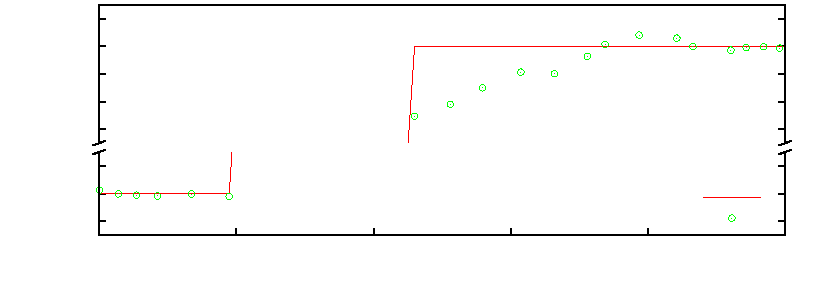
\includegraphics{laserscan_LUT-reset_zoom_01}}%
    \gplfronttext
  \end{picture}%
\endgroup

	}\\
 	\subfloat[$1000\,$GHz $\rightarrow$ $-2000\,$GHz]{
		\label{subfig:laserscan_LUT-reset_zoom_02}
		% GNUPLOT: LaTeX picture with Postscript
\begingroup
  \makeatletter
  \providecommand\color[2][]{%
    \GenericError{(gnuplot) \space\space\space\@spaces}{%
      Package color not loaded in conjunction with
      terminal option `colourtext'%
    }{See the gnuplot documentation for explanation.%
    }{Either use 'blacktext' in gnuplot or load the package
      color.sty in LaTeX.}%
    \renewcommand\color[2][]{}%
  }%
  \providecommand\includegraphics[2][]{%
    \GenericError{(gnuplot) \space\space\space\@spaces}{%
      Package graphicx or graphics not loaded%
    }{See the gnuplot documentation for explanation.%
    }{The gnuplot epslatex terminal needs graphicx.sty or graphics.sty.}%
    \renewcommand\includegraphics[2][]{}%
  }%
  \providecommand\rotatebox[2]{#2}%
  \@ifundefined{ifGPcolor}{%
    \newif\ifGPcolor
    \GPcolortrue
  }{}%
  \@ifundefined{ifGPblacktext}{%
    \newif\ifGPblacktext
    \GPblacktexttrue
  }{}%
  % define a \g@addto@macro without @ in the name:
  \let\gplgaddtomacro\g@addto@macro
  % define empty templates for all commands taking text:
  \gdef\gplbacktext{}%
  \gdef\gplfronttext{}%
  \makeatother
  \ifGPblacktext
    % no textcolor at all
    \def\colorrgb#1{}%
    \def\colorgray#1{}%
  \else
    % gray or color?
    \ifGPcolor
      \def\colorrgb#1{\color[rgb]{#1}}%
      \def\colorgray#1{\color[gray]{#1}}%
      \expandafter\def\csname LTw\endcsname{\color{white}}%
      \expandafter\def\csname LTb\endcsname{\color{black}}%
      \expandafter\def\csname LTa\endcsname{\color{black}}%
      \expandafter\def\csname LT0\endcsname{\color[rgb]{1,0,0}}%
      \expandafter\def\csname LT1\endcsname{\color[rgb]{0,1,0}}%
      \expandafter\def\csname LT2\endcsname{\color[rgb]{0,0,1}}%
      \expandafter\def\csname LT3\endcsname{\color[rgb]{1,0,1}}%
      \expandafter\def\csname LT4\endcsname{\color[rgb]{0,1,1}}%
      \expandafter\def\csname LT5\endcsname{\color[rgb]{1,1,0}}%
      \expandafter\def\csname LT6\endcsname{\color[rgb]{0,0,0}}%
      \expandafter\def\csname LT7\endcsname{\color[rgb]{1,0.3,0}}%
      \expandafter\def\csname LT8\endcsname{\color[rgb]{0.5,0.5,0.5}}%
    \else
      % gray
      \def\colorrgb#1{\color{black}}%
      \def\colorgray#1{\color[gray]{#1}}%
      \expandafter\def\csname LTw\endcsname{\color{white}}%
      \expandafter\def\csname LTb\endcsname{\color{black}}%
      \expandafter\def\csname LTa\endcsname{\color{black}}%
      \expandafter\def\csname LT0\endcsname{\color{black}}%
      \expandafter\def\csname LT1\endcsname{\color{black}}%
      \expandafter\def\csname LT2\endcsname{\color{black}}%
      \expandafter\def\csname LT3\endcsname{\color{black}}%
      \expandafter\def\csname LT4\endcsname{\color{black}}%
      \expandafter\def\csname LT5\endcsname{\color{black}}%
      \expandafter\def\csname LT6\endcsname{\color{black}}%
      \expandafter\def\csname LT7\endcsname{\color{black}}%
      \expandafter\def\csname LT8\endcsname{\color{black}}%
    \fi
  \fi
  \setlength{\unitlength}{0.0500bp}%
  \begin{picture}(7936.00,2834.00)%
    \gplgaddtomacro\gplbacktext{%
      \csname LTb\endcsname%
      \put(832,699){\makebox(0,0)[r]{\strut{}-2060}}%
      \put(832,964){\makebox(0,0)[r]{\strut{}-2040}}%
      \put(832,1230){\makebox(0,0)[r]{\strut{}-2020}}%
      \put(832,1496){\makebox(0,0)[r]{\strut{}-2000}}%
      \put(832,1761){\makebox(0,0)[r]{\strut{}-1980}}%
      \put(952,366){\makebox(0,0){\strut{} 24}}%
      \put(1775,366){\makebox(0,0){\strut{} 25}}%
      \put(2599,366){\makebox(0,0){\strut{} 26}}%
      \put(3422,366){\makebox(0,0){\strut{} 27}}%
      \put(4245,366){\makebox(0,0){\strut{} 28}}%
      \put(5068,366){\makebox(0,0){\strut{} 29}}%
      \put(5892,366){\makebox(0,0){\strut{} 30}}%
      \put(6715,366){\makebox(0,0){\strut{} 31}}%
      \put(7538,366){\makebox(0,0){\strut{} 32}}%
      \put(4245,166){\makebox(0,0){\strut{}Zeit [s]}}%
    }%
    \gplgaddtomacro\gplfronttext{%
    }%
    \gplgaddtomacro\gplbacktext{%
      \csname LTb\endcsname%
      \put(832,2113){\makebox(0,0)[r]{\strut{} 980}}%
      \put(832,2378){\makebox(0,0)[r]{\strut{} 1000}}%
      \put(832,2643){\makebox(0,0)[r]{\strut{} 1020}}%
      \put(238,371){\rotatebox{90}{\makebox(0,0)[l]{\strut{}Frequenzverschiebung [MHz]}}}%
    }%
    \gplgaddtomacro\gplfronttext{%
      \csname LTb\endcsname%
      \put(6635,2613){\makebox(0,0)[r]{\strut{}Soll-Frequenz}}%
      \csname LTb\endcsname%
      \put(6635,2413){\makebox(0,0)[r]{\strut{}Ist-Frequenz}}%
    }%
    \gplbacktext
    \put(0,0){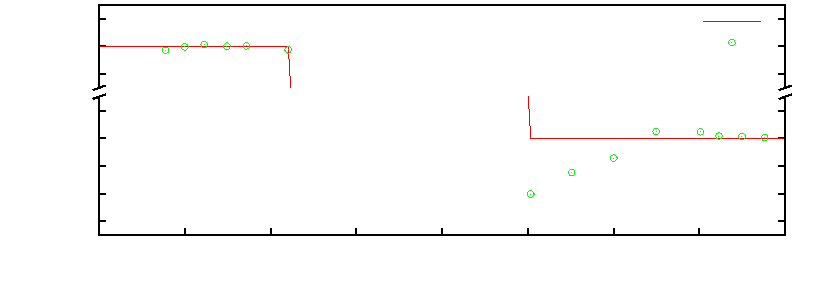
\includegraphics{laserscan_LUT-reset_zoom_02}}%
    \gplfronttext
  \end{picture}%
\endgroup

	}\\
	\subfloat[$-2000\,$GHz $\rightarrow$ $2000\,$GHz]{
		\label{subfig:laserscan_LUT-reset_zoom_03}
		% GNUPLOT: LaTeX picture with Postscript
\begingroup
  \makeatletter
  \providecommand\color[2][]{%
    \GenericError{(gnuplot) \space\space\space\@spaces}{%
      Package color not loaded in conjunction with
      terminal option `colourtext'%
    }{See the gnuplot documentation for explanation.%
    }{Either use 'blacktext' in gnuplot or load the package
      color.sty in LaTeX.}%
    \renewcommand\color[2][]{}%
  }%
  \providecommand\includegraphics[2][]{%
    \GenericError{(gnuplot) \space\space\space\@spaces}{%
      Package graphicx or graphics not loaded%
    }{See the gnuplot documentation for explanation.%
    }{The gnuplot epslatex terminal needs graphicx.sty or graphics.sty.}%
    \renewcommand\includegraphics[2][]{}%
  }%
  \providecommand\rotatebox[2]{#2}%
  \@ifundefined{ifGPcolor}{%
    \newif\ifGPcolor
    \GPcolortrue
  }{}%
  \@ifundefined{ifGPblacktext}{%
    \newif\ifGPblacktext
    \GPblacktexttrue
  }{}%
  % define a \g@addto@macro without @ in the name:
  \let\gplgaddtomacro\g@addto@macro
  % define empty templates for all commands taking text:
  \gdef\gplbacktext{}%
  \gdef\gplfronttext{}%
  \makeatother
  \ifGPblacktext
    % no textcolor at all
    \def\colorrgb#1{}%
    \def\colorgray#1{}%
  \else
    % gray or color?
    \ifGPcolor
      \def\colorrgb#1{\color[rgb]{#1}}%
      \def\colorgray#1{\color[gray]{#1}}%
      \expandafter\def\csname LTw\endcsname{\color{white}}%
      \expandafter\def\csname LTb\endcsname{\color{black}}%
      \expandafter\def\csname LTa\endcsname{\color{black}}%
      \expandafter\def\csname LT0\endcsname{\color[rgb]{1,0,0}}%
      \expandafter\def\csname LT1\endcsname{\color[rgb]{0,1,0}}%
      \expandafter\def\csname LT2\endcsname{\color[rgb]{0,0,1}}%
      \expandafter\def\csname LT3\endcsname{\color[rgb]{1,0,1}}%
      \expandafter\def\csname LT4\endcsname{\color[rgb]{0,1,1}}%
      \expandafter\def\csname LT5\endcsname{\color[rgb]{1,1,0}}%
      \expandafter\def\csname LT6\endcsname{\color[rgb]{0,0,0}}%
      \expandafter\def\csname LT7\endcsname{\color[rgb]{1,0.3,0}}%
      \expandafter\def\csname LT8\endcsname{\color[rgb]{0.5,0.5,0.5}}%
    \else
      % gray
      \def\colorrgb#1{\color{black}}%
      \def\colorgray#1{\color[gray]{#1}}%
      \expandafter\def\csname LTw\endcsname{\color{white}}%
      \expandafter\def\csname LTb\endcsname{\color{black}}%
      \expandafter\def\csname LTa\endcsname{\color{black}}%
      \expandafter\def\csname LT0\endcsname{\color{black}}%
      \expandafter\def\csname LT1\endcsname{\color{black}}%
      \expandafter\def\csname LT2\endcsname{\color{black}}%
      \expandafter\def\csname LT3\endcsname{\color{black}}%
      \expandafter\def\csname LT4\endcsname{\color{black}}%
      \expandafter\def\csname LT5\endcsname{\color{black}}%
      \expandafter\def\csname LT6\endcsname{\color{black}}%
      \expandafter\def\csname LT7\endcsname{\color{black}}%
      \expandafter\def\csname LT8\endcsname{\color{black}}%
    \fi
  \fi
  \setlength{\unitlength}{0.0500bp}%
  \begin{picture}(7936.00,2834.00)%
    \gplgaddtomacro\gplbacktext{%
      \csname LTb\endcsname%
      \put(832,718){\makebox(0,0)[r]{\strut{}-2020}}%
      \put(832,1022){\makebox(0,0)[r]{\strut{}-2000}}%
      \put(832,1325){\makebox(0,0)[r]{\strut{}-1980}}%
      \put(952,366){\makebox(0,0){\strut{} 36}}%
      \put(1684,366){\makebox(0,0){\strut{} 37}}%
      \put(2416,366){\makebox(0,0){\strut{} 38}}%
      \put(3147,366){\makebox(0,0){\strut{} 39}}%
      \put(3879,366){\makebox(0,0){\strut{} 40}}%
      \put(4611,366){\makebox(0,0){\strut{} 41}}%
      \put(5343,366){\makebox(0,0){\strut{} 42}}%
      \put(6074,366){\makebox(0,0){\strut{} 43}}%
      \put(6806,366){\makebox(0,0){\strut{} 44}}%
      \put(7538,366){\makebox(0,0){\strut{} 45}}%
      \put(4245,166){\makebox(0,0){\strut{}Zeit [s]}}%
    }%
    \gplgaddtomacro\gplfronttext{%
      \csname LTb\endcsname%
      \put(6635,929){\makebox(0,0)[r]{\strut{}Soll-Frequenz}}%
      \csname LTb\endcsname%
      \put(6635,729){\makebox(0,0)[r]{\strut{}Ist-Frequenz}}%
    }%
    \gplgaddtomacro\gplbacktext{%
      \csname LTb\endcsname%
      \put(832,1714){\makebox(0,0)[r]{\strut{} 1980}}%
      \put(832,2017){\makebox(0,0)[r]{\strut{} 2000}}%
      \put(832,2321){\makebox(0,0)[r]{\strut{} 2020}}%
      \put(832,2624){\makebox(0,0)[r]{\strut{} 2040}}%
      \put(238,371){\rotatebox{90}{\makebox(0,0)[l]{\strut{}Frequenzverschiebung [MHz]}}}%
    }%
    \gplgaddtomacro\gplfronttext{%
    }%
    \gplbacktext
    \put(0,0){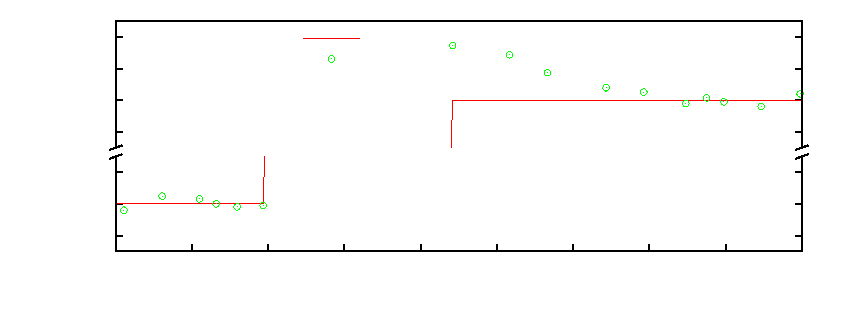
\includegraphics{laserscan_LUT-reset_zoom_03}}%
    \gplfronttext
  \end{picture}%
\endgroup

	}\\
	\subfloat[$2000\,$GHz $\rightarrow$ $-3000\,$GHz]{
		\label{subfig:laserscan_LUT-reset_zoom_04}
		% GNUPLOT: LaTeX picture with Postscript
\begingroup
  \makeatletter
  \providecommand\color[2][]{%
    \GenericError{(gnuplot) \space\space\space\@spaces}{%
      Package color not loaded in conjunction with
      terminal option `colourtext'%
    }{See the gnuplot documentation for explanation.%
    }{Either use 'blacktext' in gnuplot or load the package
      color.sty in LaTeX.}%
    \renewcommand\color[2][]{}%
  }%
  \providecommand\includegraphics[2][]{%
    \GenericError{(gnuplot) \space\space\space\@spaces}{%
      Package graphicx or graphics not loaded%
    }{See the gnuplot documentation for explanation.%
    }{The gnuplot epslatex terminal needs graphicx.sty or graphics.sty.}%
    \renewcommand\includegraphics[2][]{}%
  }%
  \providecommand\rotatebox[2]{#2}%
  \@ifundefined{ifGPcolor}{%
    \newif\ifGPcolor
    \GPcolortrue
  }{}%
  \@ifundefined{ifGPblacktext}{%
    \newif\ifGPblacktext
    \GPblacktexttrue
  }{}%
  % define a \g@addto@macro without @ in the name:
  \let\gplgaddtomacro\g@addto@macro
  % define empty templates for all commands taking text:
  \gdef\gplbacktext{}%
  \gdef\gplfronttext{}%
  \makeatother
  \ifGPblacktext
    % no textcolor at all
    \def\colorrgb#1{}%
    \def\colorgray#1{}%
  \else
    % gray or color?
    \ifGPcolor
      \def\colorrgb#1{\color[rgb]{#1}}%
      \def\colorgray#1{\color[gray]{#1}}%
      \expandafter\def\csname LTw\endcsname{\color{white}}%
      \expandafter\def\csname LTb\endcsname{\color{black}}%
      \expandafter\def\csname LTa\endcsname{\color{black}}%
      \expandafter\def\csname LT0\endcsname{\color[rgb]{1,0,0}}%
      \expandafter\def\csname LT1\endcsname{\color[rgb]{0,1,0}}%
      \expandafter\def\csname LT2\endcsname{\color[rgb]{0,0,1}}%
      \expandafter\def\csname LT3\endcsname{\color[rgb]{1,0,1}}%
      \expandafter\def\csname LT4\endcsname{\color[rgb]{0,1,1}}%
      \expandafter\def\csname LT5\endcsname{\color[rgb]{1,1,0}}%
      \expandafter\def\csname LT6\endcsname{\color[rgb]{0,0,0}}%
      \expandafter\def\csname LT7\endcsname{\color[rgb]{1,0.3,0}}%
      \expandafter\def\csname LT8\endcsname{\color[rgb]{0.5,0.5,0.5}}%
    \else
      % gray
      \def\colorrgb#1{\color{black}}%
      \def\colorgray#1{\color[gray]{#1}}%
      \expandafter\def\csname LTw\endcsname{\color{white}}%
      \expandafter\def\csname LTb\endcsname{\color{black}}%
      \expandafter\def\csname LTa\endcsname{\color{black}}%
      \expandafter\def\csname LT0\endcsname{\color{black}}%
      \expandafter\def\csname LT1\endcsname{\color{black}}%
      \expandafter\def\csname LT2\endcsname{\color{black}}%
      \expandafter\def\csname LT3\endcsname{\color{black}}%
      \expandafter\def\csname LT4\endcsname{\color{black}}%
      \expandafter\def\csname LT5\endcsname{\color{black}}%
      \expandafter\def\csname LT6\endcsname{\color{black}}%
      \expandafter\def\csname LT7\endcsname{\color{black}}%
      \expandafter\def\csname LT8\endcsname{\color{black}}%
    \fi
  \fi
  \setlength{\unitlength}{0.0500bp}%
  \begin{picture}(7936.00,2834.00)%
    \gplgaddtomacro\gplbacktext{%
      \csname LTb\endcsname%
      \put(832,699){\makebox(0,0)[r]{\strut{}-3080}}%
      \put(832,964){\makebox(0,0)[r]{\strut{}-3060}}%
      \put(832,1230){\makebox(0,0)[r]{\strut{}-3040}}%
      \put(832,1496){\makebox(0,0)[r]{\strut{}-3020}}%
      \put(832,1761){\makebox(0,0)[r]{\strut{}-3000}}%
      \put(952,366){\makebox(0,0){\strut{} 48}}%
      \put(2050,366){\makebox(0,0){\strut{} 49}}%
      \put(3147,366){\makebox(0,0){\strut{} 50}}%
      \put(4245,366){\makebox(0,0){\strut{} 51}}%
      \put(5343,366){\makebox(0,0){\strut{} 52}}%
      \put(6440,366){\makebox(0,0){\strut{} 53}}%
      \put(7538,366){\makebox(0,0){\strut{} 54}}%
      \put(4245,166){\makebox(0,0){\strut{}Zeit [s]}}%
    }%
    \gplgaddtomacro\gplfronttext{%
    }%
    \gplgaddtomacro\gplbacktext{%
      \csname LTb\endcsname%
      \put(832,2113){\makebox(0,0)[r]{\strut{} 1980}}%
      \put(832,2378){\makebox(0,0)[r]{\strut{} 2000}}%
      \put(832,2643){\makebox(0,0)[r]{\strut{} 2020}}%
      \put(238,621){\rotatebox{90}{\makebox(0,0)[l]{\strut{}Relativfrequenz [MHz]}}}%
    }%
    \gplgaddtomacro\gplfronttext{%
      \csname LTb\endcsname%
      \put(6635,2613){\makebox(0,0)[r]{\strut{}Soll-Frequenz}}%
      \csname LTb\endcsname%
      \put(6635,2413){\makebox(0,0)[r]{\strut{}Ist-Frequenz}}%
    }%
    \gplbacktext
    \put(0,0){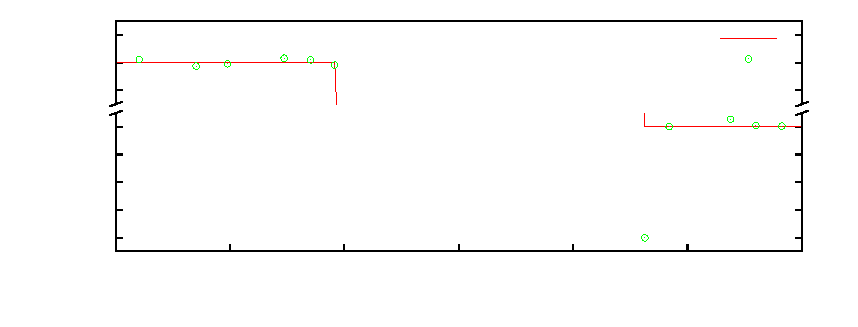
\includegraphics{laserscan_LUT-reset_zoom_04}}%
    \gplfronttext
  \end{picture}%
\endgroup

	}
	}}
	\caption[Frequenzscan, nichtlineares \textit{iScan}, vergrößert]{(a) bis (d)
	zeigen vergrößerte Ausschnitte der Frequenzverstimmungen aus Abb.
	\ref{fig:laserscan_LUT-reset}.}
	\label{fig:laserscan_LUT-reset_zoom}
\end{figure}
Bei allen Frequenzverstimmungen treten Fehler von $30$ bis $80\,$MHz unmittelbar
nach der Schrittfolge aus Tab.
\ref{tab:scan-strategie_abfolge}) auf, die von der FOL-Technik ausgeglichen
werden müssen. Die Fehler entsprechen gerade den Scanfehlern des \textit{iScans}
resultierend aus dessen Nichtlinearität. Die Gesamtverstimmungszeit liegt
zwischen $3,5$ bis $5\,$s, wobei $1$ bis $3\,$s alleine durch die Nachregelung
hervorgerufen werden. Die große Verstimmung durch die \textit{iScans}
beansprucht $2$ bis $3\,$s. Die Dauer der Nachregelung lässt sich mithilfe
der Linearisierung des \textit{iScans} verkürzen, wie sich im folgenden Abschnitt zeigt.

\subsubsection{Frequenzscans mit linearisiertem
\textit{iScan}}\label{subsubsec:frequenz_scans_lineares_iScan}
Abbildung \ref{fig:laserscan_LUT-kalibriert} zeigt
Frequenzverstimmungen mit linearisiertem \textit{iScan}. In Abb.
\ref{fig:laserscan_LUT-kalibriert_zoom} sind alle Verstimmungsschritte noch
einmal vergrößert dargestellt.
\begin{figure}[h]
	 	\centering
	 	\footnotesize
 		% GNUPLOT: LaTeX picture with Postscript
\begingroup
  \makeatletter
  \providecommand\color[2][]{%
    \GenericError{(gnuplot) \space\space\space\@spaces}{%
      Package color not loaded in conjunction with
      terminal option `colourtext'%
    }{See the gnuplot documentation for explanation.%
    }{Either use 'blacktext' in gnuplot or load the package
      color.sty in LaTeX.}%
    \renewcommand\color[2][]{}%
  }%
  \providecommand\includegraphics[2][]{%
    \GenericError{(gnuplot) \space\space\space\@spaces}{%
      Package graphicx or graphics not loaded%
    }{See the gnuplot documentation for explanation.%
    }{The gnuplot epslatex terminal needs graphicx.sty or graphics.sty.}%
    \renewcommand\includegraphics[2][]{}%
  }%
  \providecommand\rotatebox[2]{#2}%
  \@ifundefined{ifGPcolor}{%
    \newif\ifGPcolor
    \GPcolortrue
  }{}%
  \@ifundefined{ifGPblacktext}{%
    \newif\ifGPblacktext
    \GPblacktexttrue
  }{}%
  % define a \g@addto@macro without @ in the name:
  \let\gplgaddtomacro\g@addto@macro
  % define empty templates for all commands taking text:
  \gdef\gplbacktext{}%
  \gdef\gplfronttext{}%
  \makeatother
  \ifGPblacktext
    % no textcolor at all
    \def\colorrgb#1{}%
    \def\colorgray#1{}%
  \else
    % gray or color?
    \ifGPcolor
      \def\colorrgb#1{\color[rgb]{#1}}%
      \def\colorgray#1{\color[gray]{#1}}%
      \expandafter\def\csname LTw\endcsname{\color{white}}%
      \expandafter\def\csname LTb\endcsname{\color{black}}%
      \expandafter\def\csname LTa\endcsname{\color{black}}%
      \expandafter\def\csname LT0\endcsname{\color[rgb]{1,0,0}}%
      \expandafter\def\csname LT1\endcsname{\color[rgb]{0,1,0}}%
      \expandafter\def\csname LT2\endcsname{\color[rgb]{0,0,1}}%
      \expandafter\def\csname LT3\endcsname{\color[rgb]{1,0,1}}%
      \expandafter\def\csname LT4\endcsname{\color[rgb]{0,1,1}}%
      \expandafter\def\csname LT5\endcsname{\color[rgb]{1,1,0}}%
      \expandafter\def\csname LT6\endcsname{\color[rgb]{0,0,0}}%
      \expandafter\def\csname LT7\endcsname{\color[rgb]{1,0.3,0}}%
      \expandafter\def\csname LT8\endcsname{\color[rgb]{0.5,0.5,0.5}}%
    \else
      % gray
      \def\colorrgb#1{\color{black}}%
      \def\colorgray#1{\color[gray]{#1}}%
      \expandafter\def\csname LTw\endcsname{\color{white}}%
      \expandafter\def\csname LTb\endcsname{\color{black}}%
      \expandafter\def\csname LTa\endcsname{\color{black}}%
      \expandafter\def\csname LT0\endcsname{\color{black}}%
      \expandafter\def\csname LT1\endcsname{\color{black}}%
      \expandafter\def\csname LT2\endcsname{\color{black}}%
      \expandafter\def\csname LT3\endcsname{\color{black}}%
      \expandafter\def\csname LT4\endcsname{\color{black}}%
      \expandafter\def\csname LT5\endcsname{\color{black}}%
      \expandafter\def\csname LT6\endcsname{\color{black}}%
      \expandafter\def\csname LT7\endcsname{\color{black}}%
      \expandafter\def\csname LT8\endcsname{\color{black}}%
    \fi
  \fi
  \setlength{\unitlength}{0.0500bp}%
  \begin{picture}(7370.00,3968.00)%
    \gplgaddtomacro\gplbacktext{%
      \csname LTb\endcsname%
      \put(980,678){\makebox(0,0)[r]{\strut{} 0}}%
      \put(980,1059){\makebox(0,0)[r]{\strut{} 1000}}%
      \put(980,1440){\makebox(0,0)[r]{\strut{} 2000}}%
      \put(980,1821){\makebox(0,0)[r]{\strut{} 3000}}%
      \put(980,2203){\makebox(0,0)[r]{\strut{} 4000}}%
      \put(980,2584){\makebox(0,0)[r]{\strut{} 5000}}%
      \put(980,2965){\makebox(0,0)[r]{\strut{} 6000}}%
      \put(980,3346){\makebox(0,0)[r]{\strut{} 7000}}%
      \put(980,3727){\makebox(0,0)[r]{\strut{} 8000}}%
      \put(1100,440){\makebox(0,0){\strut{} 0}}%
      \put(1944,440){\makebox(0,0){\strut{} 5}}%
      \put(2788,440){\makebox(0,0){\strut{} 10}}%
      \put(3632,440){\makebox(0,0){\strut{} 15}}%
      \put(4477,440){\makebox(0,0){\strut{} 20}}%
      \put(5321,440){\makebox(0,0){\strut{} 25}}%
      \put(6165,440){\makebox(0,0){\strut{} 30}}%
      \put(7009,440){\makebox(0,0){\strut{} 35}}%
      \put(160,2183){\rotatebox{-270}{\makebox(0,0){\strut{}Frequenzverschiebung [MHz]}}}%
      \put(4054,140){\makebox(0,0){\strut{}Zeit [s]}}%
    }%
    \gplgaddtomacro\gplfronttext{%
      \csname LTb\endcsname%
      \put(6106,3564){\makebox(0,0)[r]{\strut{}Soll-Frequenz}}%
      \csname LTb\endcsname%
      \put(6106,3364){\makebox(0,0)[r]{\strut{}Ist-Frequenz}}%
    }%
    \gplbacktext
    \put(0,0){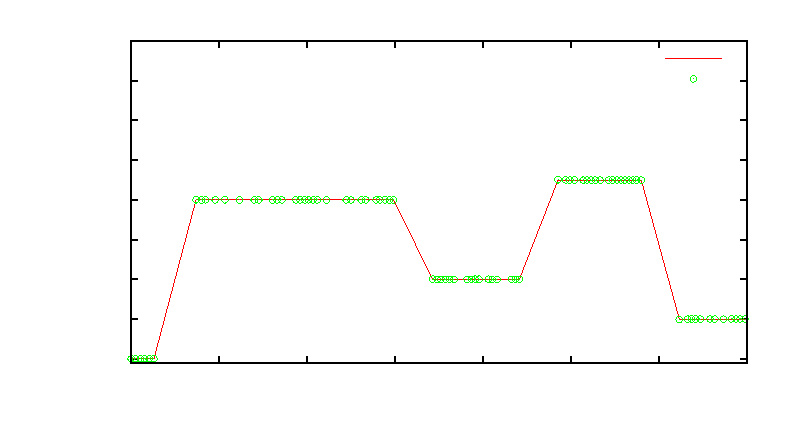
\includegraphics{laserscan_LUT-kalibriert}}%
    \gplfronttext
  \end{picture}%
\endgroup

		\caption[Frequenzscan, linearisiertes \textit{iScan}]{Mehrere
		Frequenzverstimmungen mithilfe der neu entwickelten Software und
		linearisiertem \textit{iScan}.}
		\label{fig:laserscan_LUT-kalibriert}
\end{figure}
\begin{figure}[hp]
 	\centering
 	\footnotesize
 	\fbox{\parbox{\dimexpr \linewidth - 2\fboxrule - 2\fboxsep}{
 	\subfloat[$0\,$GHz $\rightarrow$ $4000\,$GHz]{
		\label{subfig:laserscan_LUT-kalibriert_zoom_01}
		% GNUPLOT: LaTeX picture with Postscript
\begingroup
  \makeatletter
  \providecommand\color[2][]{%
    \GenericError{(gnuplot) \space\space\space\@spaces}{%
      Package color not loaded in conjunction with
      terminal option `colourtext'%
    }{See the gnuplot documentation for explanation.%
    }{Either use 'blacktext' in gnuplot or load the package
      color.sty in LaTeX.}%
    \renewcommand\color[2][]{}%
  }%
  \providecommand\includegraphics[2][]{%
    \GenericError{(gnuplot) \space\space\space\@spaces}{%
      Package graphicx or graphics not loaded%
    }{See the gnuplot documentation for explanation.%
    }{The gnuplot epslatex terminal needs graphicx.sty or graphics.sty.}%
    \renewcommand\includegraphics[2][]{}%
  }%
  \providecommand\rotatebox[2]{#2}%
  \@ifundefined{ifGPcolor}{%
    \newif\ifGPcolor
    \GPcolortrue
  }{}%
  \@ifundefined{ifGPblacktext}{%
    \newif\ifGPblacktext
    \GPblacktexttrue
  }{}%
  % define a \g@addto@macro without @ in the name:
  \let\gplgaddtomacro\g@addto@macro
  % define empty templates for all commands taking text:
  \gdef\gplbacktext{}%
  \gdef\gplfronttext{}%
  \makeatother
  \ifGPblacktext
    % no textcolor at all
    \def\colorrgb#1{}%
    \def\colorgray#1{}%
  \else
    % gray or color?
    \ifGPcolor
      \def\colorrgb#1{\color[rgb]{#1}}%
      \def\colorgray#1{\color[gray]{#1}}%
      \expandafter\def\csname LTw\endcsname{\color{white}}%
      \expandafter\def\csname LTb\endcsname{\color{black}}%
      \expandafter\def\csname LTa\endcsname{\color{black}}%
      \expandafter\def\csname LT0\endcsname{\color[rgb]{1,0,0}}%
      \expandafter\def\csname LT1\endcsname{\color[rgb]{0,1,0}}%
      \expandafter\def\csname LT2\endcsname{\color[rgb]{0,0,1}}%
      \expandafter\def\csname LT3\endcsname{\color[rgb]{1,0,1}}%
      \expandafter\def\csname LT4\endcsname{\color[rgb]{0,1,1}}%
      \expandafter\def\csname LT5\endcsname{\color[rgb]{1,1,0}}%
      \expandafter\def\csname LT6\endcsname{\color[rgb]{0,0,0}}%
      \expandafter\def\csname LT7\endcsname{\color[rgb]{1,0.3,0}}%
      \expandafter\def\csname LT8\endcsname{\color[rgb]{0.5,0.5,0.5}}%
    \else
      % gray
      \def\colorrgb#1{\color{black}}%
      \def\colorgray#1{\color[gray]{#1}}%
      \expandafter\def\csname LTw\endcsname{\color{white}}%
      \expandafter\def\csname LTb\endcsname{\color{black}}%
      \expandafter\def\csname LTa\endcsname{\color{black}}%
      \expandafter\def\csname LT0\endcsname{\color{black}}%
      \expandafter\def\csname LT1\endcsname{\color{black}}%
      \expandafter\def\csname LT2\endcsname{\color{black}}%
      \expandafter\def\csname LT3\endcsname{\color{black}}%
      \expandafter\def\csname LT4\endcsname{\color{black}}%
      \expandafter\def\csname LT5\endcsname{\color{black}}%
      \expandafter\def\csname LT6\endcsname{\color{black}}%
      \expandafter\def\csname LT7\endcsname{\color{black}}%
      \expandafter\def\csname LT8\endcsname{\color{black}}%
    \fi
  \fi
  \setlength{\unitlength}{0.0500bp}%
  \begin{picture}(7936.00,2834.00)%
    \gplgaddtomacro\gplbacktext{%
      \csname LTb\endcsname%
      \put(832,718){\makebox(0,0)[r]{\strut{}-5}}%
      \put(832,1097){\makebox(0,0)[r]{\strut{} 0}}%
      \put(832,1476){\makebox(0,0)[r]{\strut{} 5}}%
      \put(952,366){\makebox(0,0){\strut{} 0}}%
      \put(2269,366){\makebox(0,0){\strut{} 1}}%
      \put(3586,366){\makebox(0,0){\strut{} 2}}%
      \put(4904,366){\makebox(0,0){\strut{} 3}}%
      \put(6221,366){\makebox(0,0){\strut{} 4}}%
      \put(7538,366){\makebox(0,0){\strut{} 5}}%
      \put(4245,166){\makebox(0,0){\strut{}Zeit [s]}}%
    }%
    \gplgaddtomacro\gplfronttext{%
      \csname LTb\endcsname%
      \put(6635,929){\makebox(0,0)[r]{\strut{}Soll-Frequenz}}%
      \csname LTb\endcsname%
      \put(6635,729){\makebox(0,0)[r]{\strut{}Ist-Frequenz}}%
    }%
    \gplgaddtomacro\gplbacktext{%
      \csname LTb\endcsname%
      \put(832,1866){\makebox(0,0)[r]{\strut{} 3995}}%
      \put(832,2245){\makebox(0,0)[r]{\strut{} 4000}}%
      \put(832,2624){\makebox(0,0)[r]{\strut{} 4005}}%
      \put(238,371){\rotatebox{90}{\makebox(0,0)[l]{\strut{}Frequenzverschiebung [MHz]}}}%
    }%
    \gplgaddtomacro\gplfronttext{%
    }%
    \gplbacktext
    \put(0,0){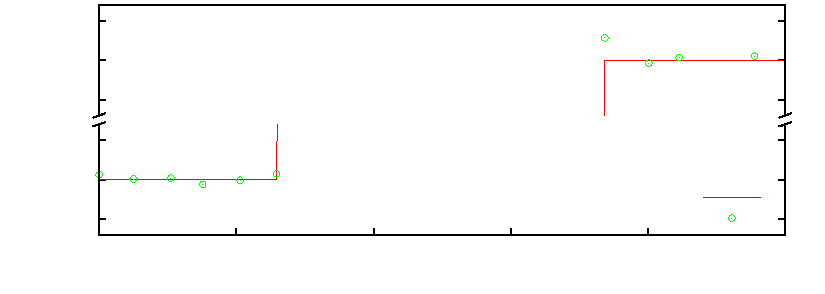
\includegraphics{laserscan_LUT-kalibriert_zoom_01}}%
    \gplfronttext
  \end{picture}%
\endgroup

	}\\
 	\subfloat[$4000\,$GHz $\rightarrow$ $2000\,$GHz]{
		\label{subfig:laserscan_LUT-kalibriert_zoom_02}
		% GNUPLOT: LaTeX picture with Postscript
\begingroup
  \makeatletter
  \providecommand\color[2][]{%
    \GenericError{(gnuplot) \space\space\space\@spaces}{%
      Package color not loaded in conjunction with
      terminal option `colourtext'%
    }{See the gnuplot documentation for explanation.%
    }{Either use 'blacktext' in gnuplot or load the package
      color.sty in LaTeX.}%
    \renewcommand\color[2][]{}%
  }%
  \providecommand\includegraphics[2][]{%
    \GenericError{(gnuplot) \space\space\space\@spaces}{%
      Package graphicx or graphics not loaded%
    }{See the gnuplot documentation for explanation.%
    }{The gnuplot epslatex terminal needs graphicx.sty or graphics.sty.}%
    \renewcommand\includegraphics[2][]{}%
  }%
  \providecommand\rotatebox[2]{#2}%
  \@ifundefined{ifGPcolor}{%
    \newif\ifGPcolor
    \GPcolortrue
  }{}%
  \@ifundefined{ifGPblacktext}{%
    \newif\ifGPblacktext
    \GPblacktexttrue
  }{}%
  % define a \g@addto@macro without @ in the name:
  \let\gplgaddtomacro\g@addto@macro
  % define empty templates for all commands taking text:
  \gdef\gplbacktext{}%
  \gdef\gplfronttext{}%
  \makeatother
  \ifGPblacktext
    % no textcolor at all
    \def\colorrgb#1{}%
    \def\colorgray#1{}%
  \else
    % gray or color?
    \ifGPcolor
      \def\colorrgb#1{\color[rgb]{#1}}%
      \def\colorgray#1{\color[gray]{#1}}%
      \expandafter\def\csname LTw\endcsname{\color{white}}%
      \expandafter\def\csname LTb\endcsname{\color{black}}%
      \expandafter\def\csname LTa\endcsname{\color{black}}%
      \expandafter\def\csname LT0\endcsname{\color[rgb]{1,0,0}}%
      \expandafter\def\csname LT1\endcsname{\color[rgb]{0,1,0}}%
      \expandafter\def\csname LT2\endcsname{\color[rgb]{0,0,1}}%
      \expandafter\def\csname LT3\endcsname{\color[rgb]{1,0,1}}%
      \expandafter\def\csname LT4\endcsname{\color[rgb]{0,1,1}}%
      \expandafter\def\csname LT5\endcsname{\color[rgb]{1,1,0}}%
      \expandafter\def\csname LT6\endcsname{\color[rgb]{0,0,0}}%
      \expandafter\def\csname LT7\endcsname{\color[rgb]{1,0.3,0}}%
      \expandafter\def\csname LT8\endcsname{\color[rgb]{0.5,0.5,0.5}}%
    \else
      % gray
      \def\colorrgb#1{\color{black}}%
      \def\colorgray#1{\color[gray]{#1}}%
      \expandafter\def\csname LTw\endcsname{\color{white}}%
      \expandafter\def\csname LTb\endcsname{\color{black}}%
      \expandafter\def\csname LTa\endcsname{\color{black}}%
      \expandafter\def\csname LT0\endcsname{\color{black}}%
      \expandafter\def\csname LT1\endcsname{\color{black}}%
      \expandafter\def\csname LT2\endcsname{\color{black}}%
      \expandafter\def\csname LT3\endcsname{\color{black}}%
      \expandafter\def\csname LT4\endcsname{\color{black}}%
      \expandafter\def\csname LT5\endcsname{\color{black}}%
      \expandafter\def\csname LT6\endcsname{\color{black}}%
      \expandafter\def\csname LT7\endcsname{\color{black}}%
      \expandafter\def\csname LT8\endcsname{\color{black}}%
    \fi
  \fi
  \setlength{\unitlength}{0.0500bp}%
  \begin{picture}(7936.00,2834.00)%
    \gplgaddtomacro\gplbacktext{%
      \csname LTb\endcsname%
      \put(832,718){\makebox(0,0)[r]{\strut{} 1995}}%
      \put(832,1097){\makebox(0,0)[r]{\strut{} 2000}}%
      \put(832,1476){\makebox(0,0)[r]{\strut{} 2005}}%
      \put(952,366){\makebox(0,0){\strut{} 13}}%
      \put(2269,366){\makebox(0,0){\strut{} 14}}%
      \put(3586,366){\makebox(0,0){\strut{} 15}}%
      \put(4904,366){\makebox(0,0){\strut{} 16}}%
      \put(6221,366){\makebox(0,0){\strut{} 17}}%
      \put(7538,366){\makebox(0,0){\strut{} 18}}%
      \put(4245,166){\makebox(0,0){\strut{}Zeit [s]}}%
    }%
    \gplgaddtomacro\gplfronttext{%
    }%
    \gplgaddtomacro\gplbacktext{%
      \csname LTb\endcsname%
      \put(832,1866){\makebox(0,0)[r]{\strut{} 3995}}%
      \put(832,2245){\makebox(0,0)[r]{\strut{} 4000}}%
      \put(832,2624){\makebox(0,0)[r]{\strut{} 4005}}%
      \put(238,371){\rotatebox{90}{\makebox(0,0)[l]{\strut{}Frequenzverschiebung [MHz]}}}%
    }%
    \gplgaddtomacro\gplfronttext{%
      \csname LTb\endcsname%
      \put(6635,2613){\makebox(0,0)[r]{\strut{}Soll-Frequenz}}%
      \csname LTb\endcsname%
      \put(6635,2413){\makebox(0,0)[r]{\strut{}Ist-Frequenz}}%
    }%
    \gplbacktext
    \put(0,0){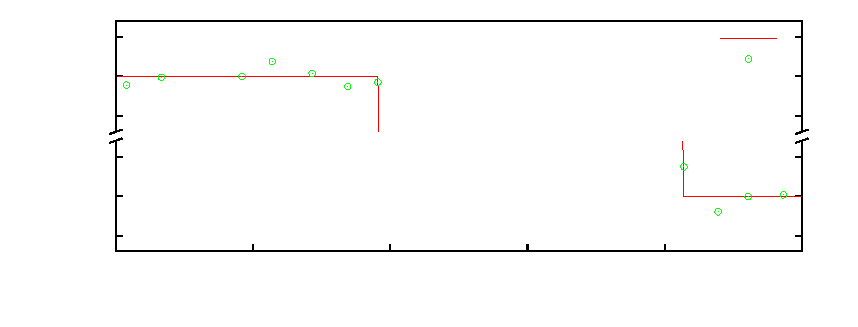
\includegraphics{laserscan_LUT-kalibriert_zoom_02}}%
    \gplfronttext
  \end{picture}%
\endgroup

	}\\
	\subfloat[$2000\,$GHz $\rightarrow$ $4500\,$GHz]{
		\label{subfig:laserscan_LUT-kalibriert_zoom_03}
		% GNUPLOT: LaTeX picture with Postscript
\begingroup
  \makeatletter
  \providecommand\color[2][]{%
    \GenericError{(gnuplot) \space\space\space\@spaces}{%
      Package color not loaded in conjunction with
      terminal option `colourtext'%
    }{See the gnuplot documentation for explanation.%
    }{Either use 'blacktext' in gnuplot or load the package
      color.sty in LaTeX.}%
    \renewcommand\color[2][]{}%
  }%
  \providecommand\includegraphics[2][]{%
    \GenericError{(gnuplot) \space\space\space\@spaces}{%
      Package graphicx or graphics not loaded%
    }{See the gnuplot documentation for explanation.%
    }{The gnuplot epslatex terminal needs graphicx.sty or graphics.sty.}%
    \renewcommand\includegraphics[2][]{}%
  }%
  \providecommand\rotatebox[2]{#2}%
  \@ifundefined{ifGPcolor}{%
    \newif\ifGPcolor
    \GPcolortrue
  }{}%
  \@ifundefined{ifGPblacktext}{%
    \newif\ifGPblacktext
    \GPblacktexttrue
  }{}%
  % define a \g@addto@macro without @ in the name:
  \let\gplgaddtomacro\g@addto@macro
  % define empty templates for all commands taking text:
  \gdef\gplbacktext{}%
  \gdef\gplfronttext{}%
  \makeatother
  \ifGPblacktext
    % no textcolor at all
    \def\colorrgb#1{}%
    \def\colorgray#1{}%
  \else
    % gray or color?
    \ifGPcolor
      \def\colorrgb#1{\color[rgb]{#1}}%
      \def\colorgray#1{\color[gray]{#1}}%
      \expandafter\def\csname LTw\endcsname{\color{white}}%
      \expandafter\def\csname LTb\endcsname{\color{black}}%
      \expandafter\def\csname LTa\endcsname{\color{black}}%
      \expandafter\def\csname LT0\endcsname{\color[rgb]{1,0,0}}%
      \expandafter\def\csname LT1\endcsname{\color[rgb]{0,1,0}}%
      \expandafter\def\csname LT2\endcsname{\color[rgb]{0,0,1}}%
      \expandafter\def\csname LT3\endcsname{\color[rgb]{1,0,1}}%
      \expandafter\def\csname LT4\endcsname{\color[rgb]{0,1,1}}%
      \expandafter\def\csname LT5\endcsname{\color[rgb]{1,1,0}}%
      \expandafter\def\csname LT6\endcsname{\color[rgb]{0,0,0}}%
      \expandafter\def\csname LT7\endcsname{\color[rgb]{1,0.3,0}}%
      \expandafter\def\csname LT8\endcsname{\color[rgb]{0.5,0.5,0.5}}%
    \else
      % gray
      \def\colorrgb#1{\color{black}}%
      \def\colorgray#1{\color[gray]{#1}}%
      \expandafter\def\csname LTw\endcsname{\color{white}}%
      \expandafter\def\csname LTb\endcsname{\color{black}}%
      \expandafter\def\csname LTa\endcsname{\color{black}}%
      \expandafter\def\csname LT0\endcsname{\color{black}}%
      \expandafter\def\csname LT1\endcsname{\color{black}}%
      \expandafter\def\csname LT2\endcsname{\color{black}}%
      \expandafter\def\csname LT3\endcsname{\color{black}}%
      \expandafter\def\csname LT4\endcsname{\color{black}}%
      \expandafter\def\csname LT5\endcsname{\color{black}}%
      \expandafter\def\csname LT6\endcsname{\color{black}}%
      \expandafter\def\csname LT7\endcsname{\color{black}}%
      \expandafter\def\csname LT8\endcsname{\color{black}}%
    \fi
  \fi
  \setlength{\unitlength}{0.0500bp}%
  \begin{picture}(7936.00,2834.00)%
    \gplgaddtomacro\gplbacktext{%
      \csname LTb\endcsname%
      \put(832,695){\makebox(0,0)[r]{\strut{} 1995}}%
      \put(832,1017){\makebox(0,0)[r]{\strut{} 2000}}%
      \put(832,1339){\makebox(0,0)[r]{\strut{} 2005}}%
      \put(952,366){\makebox(0,0){\strut{} 21}}%
      \put(2269,366){\makebox(0,0){\strut{} 22}}%
      \put(3586,366){\makebox(0,0){\strut{} 23}}%
      \put(4904,366){\makebox(0,0){\strut{} 24}}%
      \put(6221,366){\makebox(0,0){\strut{} 25}}%
      \put(7538,366){\makebox(0,0){\strut{} 26}}%
      \put(4245,166){\makebox(0,0){\strut{}Zeit [s]}}%
    }%
    \gplgaddtomacro\gplfronttext{%
    }%
    \gplgaddtomacro\gplbacktext{%
      \csname LTb\endcsname%
      \put(832,1682){\makebox(0,0)[r]{\strut{} 4495}}%
      \put(832,2004){\makebox(0,0)[r]{\strut{} 4500}}%
      \put(832,2325){\makebox(0,0)[r]{\strut{} 4505}}%
      \put(832,2647){\makebox(0,0)[r]{\strut{} 4510}}%
      \put(238,621){\rotatebox{90}{\makebox(0,0)[l]{\strut{}Relativfrequenz [MHz]}}}%
    }%
    \gplgaddtomacro\gplfronttext{%
      \csname LTb\endcsname%
      \put(2632,2613){\makebox(0,0)[r]{\strut{}Soll-Frequenz}}%
      \csname LTb\endcsname%
      \put(2632,2413){\makebox(0,0)[r]{\strut{}Ist-Frequenz}}%
    }%
    \gplbacktext
    \put(0,0){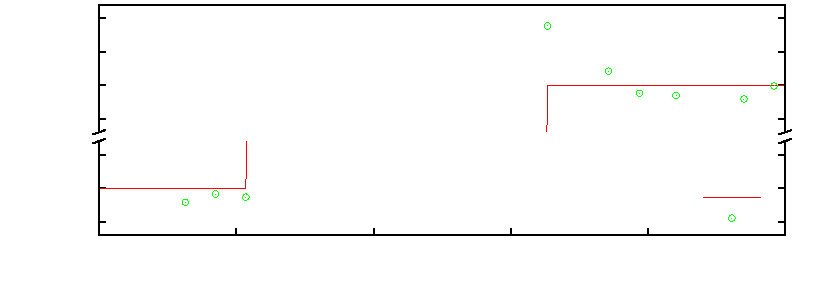
\includegraphics{laserscan_LUT-kalibriert_zoom_03}}%
    \gplfronttext
  \end{picture}%
\endgroup

	}\\
	\subfloat[$4500\,$GHz $\rightarrow$ $1000\,$GHz]{
		\label{subfig:laserscan_LUT-kalibriert_zoom_04}
		% GNUPLOT: LaTeX picture with Postscript
\begingroup
  \makeatletter
  \providecommand\color[2][]{%
    \GenericError{(gnuplot) \space\space\space\@spaces}{%
      Package color not loaded in conjunction with
      terminal option `colourtext'%
    }{See the gnuplot documentation for explanation.%
    }{Either use 'blacktext' in gnuplot or load the package
      color.sty in LaTeX.}%
    \renewcommand\color[2][]{}%
  }%
  \providecommand\includegraphics[2][]{%
    \GenericError{(gnuplot) \space\space\space\@spaces}{%
      Package graphicx or graphics not loaded%
    }{See the gnuplot documentation for explanation.%
    }{The gnuplot epslatex terminal needs graphicx.sty or graphics.sty.}%
    \renewcommand\includegraphics[2][]{}%
  }%
  \providecommand\rotatebox[2]{#2}%
  \@ifundefined{ifGPcolor}{%
    \newif\ifGPcolor
    \GPcolortrue
  }{}%
  \@ifundefined{ifGPblacktext}{%
    \newif\ifGPblacktext
    \GPblacktexttrue
  }{}%
  % define a \g@addto@macro without @ in the name:
  \let\gplgaddtomacro\g@addto@macro
  % define empty templates for all commands taking text:
  \gdef\gplbacktext{}%
  \gdef\gplfronttext{}%
  \makeatother
  \ifGPblacktext
    % no textcolor at all
    \def\colorrgb#1{}%
    \def\colorgray#1{}%
  \else
    % gray or color?
    \ifGPcolor
      \def\colorrgb#1{\color[rgb]{#1}}%
      \def\colorgray#1{\color[gray]{#1}}%
      \expandafter\def\csname LTw\endcsname{\color{white}}%
      \expandafter\def\csname LTb\endcsname{\color{black}}%
      \expandafter\def\csname LTa\endcsname{\color{black}}%
      \expandafter\def\csname LT0\endcsname{\color[rgb]{1,0,0}}%
      \expandafter\def\csname LT1\endcsname{\color[rgb]{0,1,0}}%
      \expandafter\def\csname LT2\endcsname{\color[rgb]{0,0,1}}%
      \expandafter\def\csname LT3\endcsname{\color[rgb]{1,0,1}}%
      \expandafter\def\csname LT4\endcsname{\color[rgb]{0,1,1}}%
      \expandafter\def\csname LT5\endcsname{\color[rgb]{1,1,0}}%
      \expandafter\def\csname LT6\endcsname{\color[rgb]{0,0,0}}%
      \expandafter\def\csname LT7\endcsname{\color[rgb]{1,0.3,0}}%
      \expandafter\def\csname LT8\endcsname{\color[rgb]{0.5,0.5,0.5}}%
    \else
      % gray
      \def\colorrgb#1{\color{black}}%
      \def\colorgray#1{\color[gray]{#1}}%
      \expandafter\def\csname LTw\endcsname{\color{white}}%
      \expandafter\def\csname LTb\endcsname{\color{black}}%
      \expandafter\def\csname LTa\endcsname{\color{black}}%
      \expandafter\def\csname LT0\endcsname{\color{black}}%
      \expandafter\def\csname LT1\endcsname{\color{black}}%
      \expandafter\def\csname LT2\endcsname{\color{black}}%
      \expandafter\def\csname LT3\endcsname{\color{black}}%
      \expandafter\def\csname LT4\endcsname{\color{black}}%
      \expandafter\def\csname LT5\endcsname{\color{black}}%
      \expandafter\def\csname LT6\endcsname{\color{black}}%
      \expandafter\def\csname LT7\endcsname{\color{black}}%
      \expandafter\def\csname LT8\endcsname{\color{black}}%
    \fi
  \fi
  \setlength{\unitlength}{0.0500bp}%
  \begin{picture}(7936.00,2834.00)%
    \gplgaddtomacro\gplbacktext{%
      \csname LTb\endcsname%
      \put(832,729){\makebox(0,0)[r]{\strut{} 985}}%
      \put(832,1002){\makebox(0,0)[r]{\strut{} 990}}%
      \put(832,1274){\makebox(0,0)[r]{\strut{} 995}}%
      \put(832,1547){\makebox(0,0)[r]{\strut{} 1000}}%
      \put(832,1819){\makebox(0,0)[r]{\strut{} 1005}}%
      \put(952,366){\makebox(0,0){\strut{} 28}}%
      \put(2269,366){\makebox(0,0){\strut{} 29}}%
      \put(3586,366){\makebox(0,0){\strut{} 30}}%
      \put(4904,366){\makebox(0,0){\strut{} 31}}%
      \put(6221,366){\makebox(0,0){\strut{} 32}}%
      \put(7538,366){\makebox(0,0){\strut{} 33}}%
      \put(4245,166){\makebox(0,0){\strut{}Zeit [s]}}%
    }%
    \gplgaddtomacro\gplfronttext{%
    }%
    \gplgaddtomacro\gplbacktext{%
      \csname LTb\endcsname%
      \put(832,2123){\makebox(0,0)[r]{\strut{} 4495}}%
      \put(832,2395){\makebox(0,0)[r]{\strut{} 4500}}%
      \put(832,2667){\makebox(0,0)[r]{\strut{} 4505}}%
      \put(238,621){\rotatebox{90}{\makebox(0,0)[l]{\strut{}Relativfrequenz [MHz]}}}%
    }%
    \gplgaddtomacro\gplfronttext{%
      \csname LTb\endcsname%
      \put(6635,2613){\makebox(0,0)[r]{\strut{}Soll-Frequenz}}%
      \csname LTb\endcsname%
      \put(6635,2413){\makebox(0,0)[r]{\strut{}Ist-Frequenz}}%
    }%
    \gplbacktext
    \put(0,0){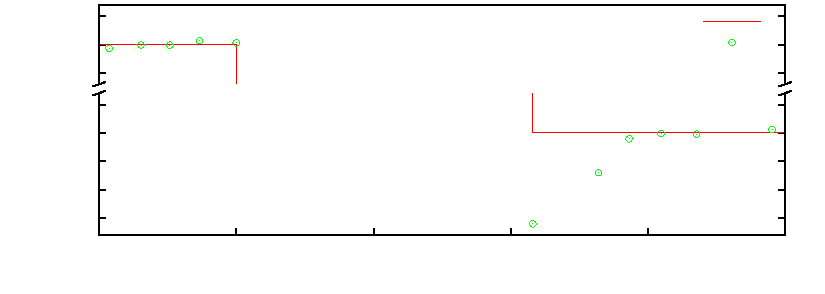
\includegraphics{laserscan_LUT-kalibriert_zoom_04}}%
    \gplfronttext
  \end{picture}%
\endgroup

	}
	}}
	\caption[Frequenzscan, linearisisiertes \textit{iScan}, vergrößert]{(a) bis (d)
	zeigen vergrößerte Ausschnitte der Frequenzverstimmungen aus Abb.
	\ref{fig:laserscan_LUT-kalibriert}.}
	\label{fig:laserscan_LUT-kalibriert_zoom}
\end{figure}
Die Messung zeigt, dass bei linearisiertem \textit{iScan} die Dauer des
Nachregelns auf $<1\,$s verkürzt wird. Die Dauer der eigentlichen
Verstimmung durch die \textit{iScans} verändert sich logischerweise nicht,
wodurch die minimale Verstimmungsdauer für beliebige Relativfrequenzen zwischen
$2$ und $3\,$s liegt.

\subsubsection{Frequenzscans im
Vergleich mit dem alten
System}\label{subsubsec:frequenz_scans_vergleich_mit_altem_system}
Im alten System war die maximale Verstimmungsgeschwindigkeit ca. $3\,$GHz pro
Sekunde ($\nicefrac{\text{FSR}}{5}$ pro Rampe, Rampenfrequenz ca. $50\,$Hz). Bei
der neu entwickelten Verstimmungstechnik hängt nur noch die Dauer des
Nachregelns durch das FOL von der Differenz von Ist- und Sollfrequenz ab. Die
Dauer des großen Teils der Verstimmung mithilfe der \textit{iScans} ist praktisch im Mittel bei jeder Differenzfrequenz gleich (ca. $2$ bis $3\,$s) und
wird durch ineffiziente Kommunikation zwischen PC und \textit{iScan control
unit} verursacht. Mit einer Gesamtverstimmungsdauer von $5\,$s, wie es beim
nichtlinearen \textit{iScan} üblich ist, würde die neue Technik im
Vergleich zur alten Technik erst bei Verstimmungen von ca. $15\,$GHz einen
Zugewinn an Geschwindigkeit bringen.
Entfällt praktisch die Verstimmungsdauer der Nachregelung durch ein
linearisiertes \textit{iScan}, wäre dies ab ca. $9\,$GHz der Fall.
Die Linearisierung bringt zwar Vorteile, reicht aber für den
Geschwindigkeitsaspekt noch nicht aus.\par
Der Grund der effektiv zu langsamen Verstimmmung liegt nicht im Prinzip der
Technik, sondern in Teilen der softwareseitigen Umsetzung. Um die Kommunikation
mit den \textit{iScans control units} fehlerfrei zu gestalten, wurden von \textit{TEM
Messtechnik} diverse Warteschleifen in die Kommunikation-VIs implementiert.
Weiterhin sind die VIs nicht reentrant, was den gleichzeitigen Zugriff zweier Prozesse auf die \textit{iScan control unit}
unterbindet, aber auch die gleichzeitige Kommunikation mit zwei \textit{iScan
control units} unnötig verlangsamt. Hier kann in Zukunft angesetzt
und ein performanteres Kommunikationsinterface entworfen werden, was mit relativ
wenig Aufwand verbunden sein sollte.

\section{Spektroskopie an Uran}\label{sec:spektroskopie}
Im Rahmen dieser Arbeit wurden abschließend spektroskopische
Untersuchungen an $^{238}$U durchgeführt, die im Folgenden diskutiert werden
sollen. Zunächst wird kurz auf das bisher verwendete Anregungsschema für
$^{238}$U im alten System eingegangen. Anschließend wird der aktuelle Status
der Suche nach neuen Anregungsschemata vorgestellt.

\subsection{Altes Anregungsschema}\label{subsec:anregungsschema_alt}
Das bisher verwendete Anregungsschema ist in Abb.
\ref{fig:anregungsschema_alt} dargestellt.
\begin{figure}[h]
 	\centering
 	\fbox{\parbox{\dimexpr \linewidth - 2\fboxrule - 2\fboxsep}{
 	\centering
	    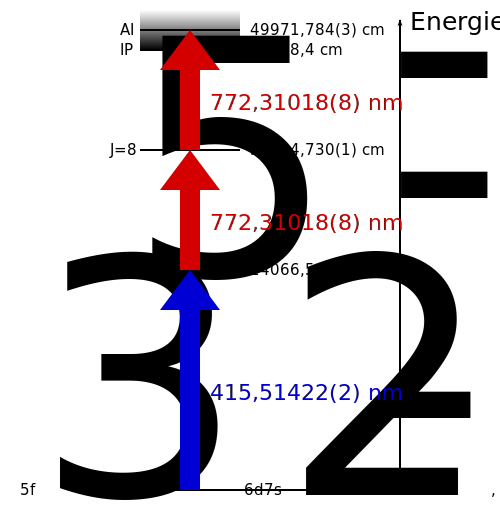
\includegraphics[width=\textwidth-7cm]{gfx/anregungsschema_alt}
	    }}
	\caption[Anregungsschema, alt]{Altes, bisher benutzten
	Anregungsschema.}
	\label{fig:anregungsschema_alt}
\end{figure}
Die Anregung in den FES aus dem Grundzustand (GZ) wurde mit
dem bisher verwendeten blauen Diodenlaser bei $415\,$nm realisiert. Da dieser
Laserdiodentyp aber nicht mehr hergestellt wird, müssen neue Schemata mit langfristig verfügbaren Laserdioden entwickelt
werden. Im alten Schema wurde über einen weiteren angeregten Zwischenzustand ein
autoionisierender Zustand (AI) besetzt, der knapp über dem Ionisationspotential (IP) liegt ($\Delta E=13,38\,$cm$^{-1}$).
Abbildung \ref{fig:linienscans_altes_schema} zeigt die Linienprofile aller drei
Übergänge, die mit dem alten System aufgenommen wurden, wobei beim jeweiligen Scan die anderen
Laser in Resonanz waren.
\begin{figure}[hp]
 	\centering
 	\footnotesize
 	\fbox{\parbox{\dimexpr \linewidth - 2\fboxrule - 2\fboxsep}{
 	\subfloat[Autoionisierender Anregungsschritt @ $771,78040(8)\,$nm]{
		\label{subfig:linienscans_altes_schema_AI}
		% GNUPLOT: LaTeX picture with Postscript
\begingroup
  \makeatletter
  \providecommand\color[2][]{%
    \GenericError{(gnuplot) \space\space\space\@spaces}{%
      Package color not loaded in conjunction with
      terminal option `colourtext'%
    }{See the gnuplot documentation for explanation.%
    }{Either use 'blacktext' in gnuplot or load the package
      color.sty in LaTeX.}%
    \renewcommand\color[2][]{}%
  }%
  \providecommand\includegraphics[2][]{%
    \GenericError{(gnuplot) \space\space\space\@spaces}{%
      Package graphicx or graphics not loaded%
    }{See the gnuplot documentation for explanation.%
    }{The gnuplot epslatex terminal needs graphicx.sty or graphics.sty.}%
    \renewcommand\includegraphics[2][]{}%
  }%
  \providecommand\rotatebox[2]{#2}%
  \@ifundefined{ifGPcolor}{%
    \newif\ifGPcolor
    \GPcolortrue
  }{}%
  \@ifundefined{ifGPblacktext}{%
    \newif\ifGPblacktext
    \GPblacktexttrue
  }{}%
  % define a \g@addto@macro without @ in the name:
  \let\gplgaddtomacro\g@addto@macro
  % define empty templates for all commands taking text:
  \gdef\gplbacktext{}%
  \gdef\gplfronttext{}%
  \makeatother
  \ifGPblacktext
    % no textcolor at all
    \def\colorrgb#1{}%
    \def\colorgray#1{}%
  \else
    % gray or color?
    \ifGPcolor
      \def\colorrgb#1{\color[rgb]{#1}}%
      \def\colorgray#1{\color[gray]{#1}}%
      \expandafter\def\csname LTw\endcsname{\color{white}}%
      \expandafter\def\csname LTb\endcsname{\color{black}}%
      \expandafter\def\csname LTa\endcsname{\color{black}}%
      \expandafter\def\csname LT0\endcsname{\color[rgb]{1,0,0}}%
      \expandafter\def\csname LT1\endcsname{\color[rgb]{0,1,0}}%
      \expandafter\def\csname LT2\endcsname{\color[rgb]{0,0,1}}%
      \expandafter\def\csname LT3\endcsname{\color[rgb]{1,0,1}}%
      \expandafter\def\csname LT4\endcsname{\color[rgb]{0,1,1}}%
      \expandafter\def\csname LT5\endcsname{\color[rgb]{1,1,0}}%
      \expandafter\def\csname LT6\endcsname{\color[rgb]{0,0,0}}%
      \expandafter\def\csname LT7\endcsname{\color[rgb]{1,0.3,0}}%
      \expandafter\def\csname LT8\endcsname{\color[rgb]{0.5,0.5,0.5}}%
    \else
      % gray
      \def\colorrgb#1{\color{black}}%
      \def\colorgray#1{\color[gray]{#1}}%
      \expandafter\def\csname LTw\endcsname{\color{white}}%
      \expandafter\def\csname LTb\endcsname{\color{black}}%
      \expandafter\def\csname LTa\endcsname{\color{black}}%
      \expandafter\def\csname LT0\endcsname{\color{black}}%
      \expandafter\def\csname LT1\endcsname{\color{black}}%
      \expandafter\def\csname LT2\endcsname{\color{black}}%
      \expandafter\def\csname LT3\endcsname{\color{black}}%
      \expandafter\def\csname LT4\endcsname{\color{black}}%
      \expandafter\def\csname LT5\endcsname{\color{black}}%
      \expandafter\def\csname LT6\endcsname{\color{black}}%
      \expandafter\def\csname LT7\endcsname{\color{black}}%
      \expandafter\def\csname LT8\endcsname{\color{black}}%
    \fi
  \fi
  \setlength{\unitlength}{0.0500bp}%
  \begin{picture}(7936.00,3968.00)%
    \gplgaddtomacro\gplbacktext{%
      \csname LTb\endcsname%
      \put(860,640){\makebox(0,0)[r]{\strut{} 0}}%
      \put(860,1005){\makebox(0,0)[r]{\strut{} 50}}%
      \put(860,1370){\makebox(0,0)[r]{\strut{} 100}}%
      \put(860,1736){\makebox(0,0)[r]{\strut{} 150}}%
      \put(860,2101){\makebox(0,0)[r]{\strut{} 200}}%
      \put(860,2466){\makebox(0,0)[r]{\strut{} 250}}%
      \put(860,2831){\makebox(0,0)[r]{\strut{} 300}}%
      \put(860,3197){\makebox(0,0)[r]{\strut{} 350}}%
      \put(860,3562){\makebox(0,0)[r]{\strut{} 400}}%
      \put(860,3927){\makebox(0,0)[r]{\strut{} 450}}%
      \put(980,440){\makebox(0,0){\strut{}-300}}%
      \put(2079,440){\makebox(0,0){\strut{}-200}}%
      \put(3178,440){\makebox(0,0){\strut{}-100}}%
      \put(4278,440){\makebox(0,0){\strut{} 0}}%
      \put(5377,440){\makebox(0,0){\strut{} 100}}%
      \put(6476,440){\makebox(0,0){\strut{} 200}}%
      \put(7575,440){\makebox(0,0){\strut{} 300}}%
      \put(160,2283){\rotatebox{-270}{\makebox(0,0){\strut{}Countrate [s$^{-1}$]}}}%
      \put(4277,140){\makebox(0,0){\strut{}Relativfrequenz [MHz]}}%
      \put(1310,3598){\makebox(0,0)[l]{\strut{}$F(\nu)=a\cdot\frac{\left(\nicefrac{q\Gamma}{2}+\nu-\nu_0\right)^2}{\left(\nu-\nu_0\right)^2+\left(\nicefrac{\Gamma}{2}\right)^2}+b$}}%
      \put(1310,3105){\makebox(0,0)[l]{\strut{}$\Gamma = (55.8\pm1.1)\,$MHz}}%
      \put(1310,2875){\makebox(0,0)[l]{\strut{}$\nu_0 = (-3.31\pm0.51)\,$MHz}}%
      \put(1310,2645){\makebox(0,0)[l]{\strut{}$q = 178\pm217$}}%
      \put(1310,2415){\makebox(0,0)[l]{\strut{}$a = (0.011\pm0.027)\,$s$^{-1}$}}%
      \put(1310,2185){\makebox(0,0)[l]{\strut{}$b = (0.7\pm1.1)\,$s$^{-1}$}}%
    }%
    \gplgaddtomacro\gplfronttext{%
      \csname LTb\endcsname%
      \put(6672,3764){\makebox(0,0)[r]{\strut{}Messpunkte}}%
      \csname LTb\endcsname%
      \put(6672,3564){\makebox(0,0)[r]{\strut{}Fit}}%
    }%
    \gplbacktext
    \put(0,0){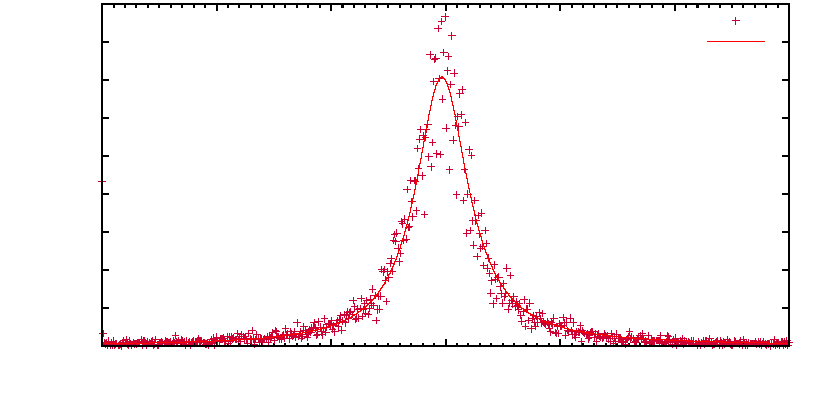
\includegraphics{linienscans_altes_schema_AI}}%
    \gplfronttext
  \end{picture}%
\endgroup

	}\\
 	\subfloat[Zweiter Anregungsschritt @ $772,31018(8)\,$nm]{
		\label{subfig:linienscans_altes_schema_SES}
		% GNUPLOT: LaTeX picture with Postscript
\begingroup
  \makeatletter
  \providecommand\color[2][]{%
    \GenericError{(gnuplot) \space\space\space\@spaces}{%
      Package color not loaded in conjunction with
      terminal option `colourtext'%
    }{See the gnuplot documentation for explanation.%
    }{Either use 'blacktext' in gnuplot or load the package
      color.sty in LaTeX.}%
    \renewcommand\color[2][]{}%
  }%
  \providecommand\includegraphics[2][]{%
    \GenericError{(gnuplot) \space\space\space\@spaces}{%
      Package graphicx or graphics not loaded%
    }{See the gnuplot documentation for explanation.%
    }{The gnuplot epslatex terminal needs graphicx.sty or graphics.sty.}%
    \renewcommand\includegraphics[2][]{}%
  }%
  \providecommand\rotatebox[2]{#2}%
  \@ifundefined{ifGPcolor}{%
    \newif\ifGPcolor
    \GPcolortrue
  }{}%
  \@ifundefined{ifGPblacktext}{%
    \newif\ifGPblacktext
    \GPblacktexttrue
  }{}%
  % define a \g@addto@macro without @ in the name:
  \let\gplgaddtomacro\g@addto@macro
  % define empty templates for all commands taking text:
  \gdef\gplbacktext{}%
  \gdef\gplfronttext{}%
  \makeatother
  \ifGPblacktext
    % no textcolor at all
    \def\colorrgb#1{}%
    \def\colorgray#1{}%
  \else
    % gray or color?
    \ifGPcolor
      \def\colorrgb#1{\color[rgb]{#1}}%
      \def\colorgray#1{\color[gray]{#1}}%
      \expandafter\def\csname LTw\endcsname{\color{white}}%
      \expandafter\def\csname LTb\endcsname{\color{black}}%
      \expandafter\def\csname LTa\endcsname{\color{black}}%
      \expandafter\def\csname LT0\endcsname{\color[rgb]{1,0,0}}%
      \expandafter\def\csname LT1\endcsname{\color[rgb]{0,1,0}}%
      \expandafter\def\csname LT2\endcsname{\color[rgb]{0,0,1}}%
      \expandafter\def\csname LT3\endcsname{\color[rgb]{1,0,1}}%
      \expandafter\def\csname LT4\endcsname{\color[rgb]{0,1,1}}%
      \expandafter\def\csname LT5\endcsname{\color[rgb]{1,1,0}}%
      \expandafter\def\csname LT6\endcsname{\color[rgb]{0,0,0}}%
      \expandafter\def\csname LT7\endcsname{\color[rgb]{1,0.3,0}}%
      \expandafter\def\csname LT8\endcsname{\color[rgb]{0.5,0.5,0.5}}%
    \else
      % gray
      \def\colorrgb#1{\color{black}}%
      \def\colorgray#1{\color[gray]{#1}}%
      \expandafter\def\csname LTw\endcsname{\color{white}}%
      \expandafter\def\csname LTb\endcsname{\color{black}}%
      \expandafter\def\csname LTa\endcsname{\color{black}}%
      \expandafter\def\csname LT0\endcsname{\color{black}}%
      \expandafter\def\csname LT1\endcsname{\color{black}}%
      \expandafter\def\csname LT2\endcsname{\color{black}}%
      \expandafter\def\csname LT3\endcsname{\color{black}}%
      \expandafter\def\csname LT4\endcsname{\color{black}}%
      \expandafter\def\csname LT5\endcsname{\color{black}}%
      \expandafter\def\csname LT6\endcsname{\color{black}}%
      \expandafter\def\csname LT7\endcsname{\color{black}}%
      \expandafter\def\csname LT8\endcsname{\color{black}}%
    \fi
  \fi
  \setlength{\unitlength}{0.0500bp}%
  \begin{picture}(7936.00,3968.00)%
    \gplgaddtomacro\gplbacktext{%
      \csname LTb\endcsname%
      \put(860,640){\makebox(0,0)[r]{\strut{} 0}}%
      \put(860,1051){\makebox(0,0)[r]{\strut{} 50}}%
      \put(860,1462){\makebox(0,0)[r]{\strut{} 100}}%
      \put(860,1873){\makebox(0,0)[r]{\strut{} 150}}%
      \put(860,2283){\makebox(0,0)[r]{\strut{} 200}}%
      \put(860,2694){\makebox(0,0)[r]{\strut{} 250}}%
      \put(860,3105){\makebox(0,0)[r]{\strut{} 300}}%
      \put(860,3516){\makebox(0,0)[r]{\strut{} 350}}%
      \put(860,3927){\makebox(0,0)[r]{\strut{} 400}}%
      \put(980,440){\makebox(0,0){\strut{}-150}}%
      \put(2079,440){\makebox(0,0){\strut{}-100}}%
      \put(3178,440){\makebox(0,0){\strut{}-50}}%
      \put(4278,440){\makebox(0,0){\strut{} 0}}%
      \put(5377,440){\makebox(0,0){\strut{} 50}}%
      \put(6476,440){\makebox(0,0){\strut{} 100}}%
      \put(7575,440){\makebox(0,0){\strut{} 150}}%
      \put(160,2283){\rotatebox{-270}{\makebox(0,0){\strut{}Countrate [s$^{-1}$]}}}%
      \put(4277,140){\makebox(0,0){\strut{}Relativfrequenz [MHz]}}%
      \put(1178,3598){\makebox(0,0)[l]{\strut{}$G(\nu)=A\cdot\frac{1}{\sigma\sqrt{2\pi}}\mathrm{e}^{-\frac{1}{2}\frac{(\nu-\mu)^2}{\sigma^2}}+b$}}%
      \put(1178,3105){\makebox(0,0)[l]{\strut{}$2\sigma = (25.37\pm0.52)\,$MHz}}%
      \put(1178,2875){\makebox(0,0)[l]{\strut{}$\mu = (-2.37\pm0.25)\,$MHz}}%
      \put(1178,2645){\makebox(0,0)[l]{\strut{}$A = (10651\pm206)\,\nicefrac{\text{MHz}}{\text{s}}$}}%
      \put(1178,2415){\makebox(0,0)[l]{\strut{}$b = (0.4\pm1.4)\,$s$^{-1}$}}%
    }%
    \gplgaddtomacro\gplfronttext{%
      \csname LTb\endcsname%
      \put(6672,3764){\makebox(0,0)[r]{\strut{}Messpunkte}}%
      \csname LTb\endcsname%
      \put(6672,3564){\makebox(0,0)[r]{\strut{}Fit}}%
    }%
    \gplbacktext
    \put(0,0){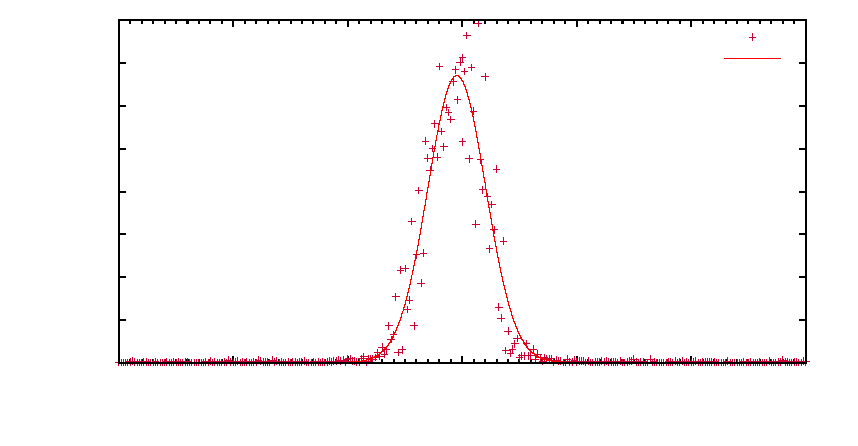
\includegraphics{linienscans_altes_schema_SES}}%
    \gplfronttext
  \end{picture}%
\endgroup

	}\\
	\subfloat[Erster Anregungsschritt @ $415,51422(2)\,$nm]{
		\label{subfig:linienscans_altes_schema_FES}
		% GNUPLOT: LaTeX picture with Postscript
\begingroup
  \makeatletter
  \providecommand\color[2][]{%
    \GenericError{(gnuplot) \space\space\space\@spaces}{%
      Package color not loaded in conjunction with
      terminal option `colourtext'%
    }{See the gnuplot documentation for explanation.%
    }{Either use 'blacktext' in gnuplot or load the package
      color.sty in LaTeX.}%
    \renewcommand\color[2][]{}%
  }%
  \providecommand\includegraphics[2][]{%
    \GenericError{(gnuplot) \space\space\space\@spaces}{%
      Package graphicx or graphics not loaded%
    }{See the gnuplot documentation for explanation.%
    }{The gnuplot epslatex terminal needs graphicx.sty or graphics.sty.}%
    \renewcommand\includegraphics[2][]{}%
  }%
  \providecommand\rotatebox[2]{#2}%
  \@ifundefined{ifGPcolor}{%
    \newif\ifGPcolor
    \GPcolortrue
  }{}%
  \@ifundefined{ifGPblacktext}{%
    \newif\ifGPblacktext
    \GPblacktexttrue
  }{}%
  % define a \g@addto@macro without @ in the name:
  \let\gplgaddtomacro\g@addto@macro
  % define empty templates for all commands taking text:
  \gdef\gplbacktext{}%
  \gdef\gplfronttext{}%
  \makeatother
  \ifGPblacktext
    % no textcolor at all
    \def\colorrgb#1{}%
    \def\colorgray#1{}%
  \else
    % gray or color?
    \ifGPcolor
      \def\colorrgb#1{\color[rgb]{#1}}%
      \def\colorgray#1{\color[gray]{#1}}%
      \expandafter\def\csname LTw\endcsname{\color{white}}%
      \expandafter\def\csname LTb\endcsname{\color{black}}%
      \expandafter\def\csname LTa\endcsname{\color{black}}%
      \expandafter\def\csname LT0\endcsname{\color[rgb]{1,0,0}}%
      \expandafter\def\csname LT1\endcsname{\color[rgb]{0,1,0}}%
      \expandafter\def\csname LT2\endcsname{\color[rgb]{0,0,1}}%
      \expandafter\def\csname LT3\endcsname{\color[rgb]{1,0,1}}%
      \expandafter\def\csname LT4\endcsname{\color[rgb]{0,1,1}}%
      \expandafter\def\csname LT5\endcsname{\color[rgb]{1,1,0}}%
      \expandafter\def\csname LT6\endcsname{\color[rgb]{0,0,0}}%
      \expandafter\def\csname LT7\endcsname{\color[rgb]{1,0.3,0}}%
      \expandafter\def\csname LT8\endcsname{\color[rgb]{0.5,0.5,0.5}}%
    \else
      % gray
      \def\colorrgb#1{\color{black}}%
      \def\colorgray#1{\color[gray]{#1}}%
      \expandafter\def\csname LTw\endcsname{\color{white}}%
      \expandafter\def\csname LTb\endcsname{\color{black}}%
      \expandafter\def\csname LTa\endcsname{\color{black}}%
      \expandafter\def\csname LT0\endcsname{\color{black}}%
      \expandafter\def\csname LT1\endcsname{\color{black}}%
      \expandafter\def\csname LT2\endcsname{\color{black}}%
      \expandafter\def\csname LT3\endcsname{\color{black}}%
      \expandafter\def\csname LT4\endcsname{\color{black}}%
      \expandafter\def\csname LT5\endcsname{\color{black}}%
      \expandafter\def\csname LT6\endcsname{\color{black}}%
      \expandafter\def\csname LT7\endcsname{\color{black}}%
      \expandafter\def\csname LT8\endcsname{\color{black}}%
    \fi
  \fi
  \setlength{\unitlength}{0.0500bp}%
  \begin{picture}(7936.00,3968.00)%
    \gplgaddtomacro\gplbacktext{%
      \csname LTb\endcsname%
      \put(860,640){\makebox(0,0)[r]{\strut{} 0}}%
      \put(860,1005){\makebox(0,0)[r]{\strut{} 50}}%
      \put(860,1370){\makebox(0,0)[r]{\strut{} 100}}%
      \put(860,1736){\makebox(0,0)[r]{\strut{} 150}}%
      \put(860,2101){\makebox(0,0)[r]{\strut{} 200}}%
      \put(860,2466){\makebox(0,0)[r]{\strut{} 250}}%
      \put(860,2831){\makebox(0,0)[r]{\strut{} 300}}%
      \put(860,3197){\makebox(0,0)[r]{\strut{} 350}}%
      \put(860,3562){\makebox(0,0)[r]{\strut{} 400}}%
      \put(860,3927){\makebox(0,0)[r]{\strut{} 450}}%
      \put(980,440){\makebox(0,0){\strut{}-150}}%
      \put(2079,440){\makebox(0,0){\strut{}-100}}%
      \put(3178,440){\makebox(0,0){\strut{}-50}}%
      \put(4278,440){\makebox(0,0){\strut{} 0}}%
      \put(5377,440){\makebox(0,0){\strut{} 50}}%
      \put(6476,440){\makebox(0,0){\strut{} 100}}%
      \put(7575,440){\makebox(0,0){\strut{} 150}}%
      \put(160,2283){\rotatebox{-270}{\makebox(0,0){\strut{}Countrate [s$^{-1}$]}}}%
      \put(4277,140){\makebox(0,0){\strut{}Relativfrequenz [MHz]}}%
      \put(1178,3598){\makebox(0,0)[l]{\strut{}$G(\nu)=A\cdot\frac{1}{\sigma\sqrt{2\pi}}\mathrm{e}^{-\frac{1}{2}\frac{(\nu-\mu)^2}{\sigma^2}}+b$}}%
      \put(1178,3105){\makebox(0,0)[l]{\strut{}$2\sigma = (39.13\pm0.83)\,$MHz}}%
      \put(1178,2875){\makebox(0,0)[l]{\strut{}$\mu = (-10.97\pm0.38)\,$MHz}}%
      \put(1178,2645){\makebox(0,0)[l]{\strut{}$A = (17938\pm376)\,\nicefrac{\text{MHz}}{\text{s}}$}}%
      \put(1178,2415){\makebox(0,0)[l]{\strut{}$b = (1.0\pm2.1)\,$s$^{-1}$}}%
    }%
    \gplgaddtomacro\gplfronttext{%
      \csname LTb\endcsname%
      \put(6672,3764){\makebox(0,0)[r]{\strut{}Messpunkte}}%
      \csname LTb\endcsname%
      \put(6672,3564){\makebox(0,0)[r]{\strut{}Fit}}%
    }%
    \gplbacktext
    \put(0,0){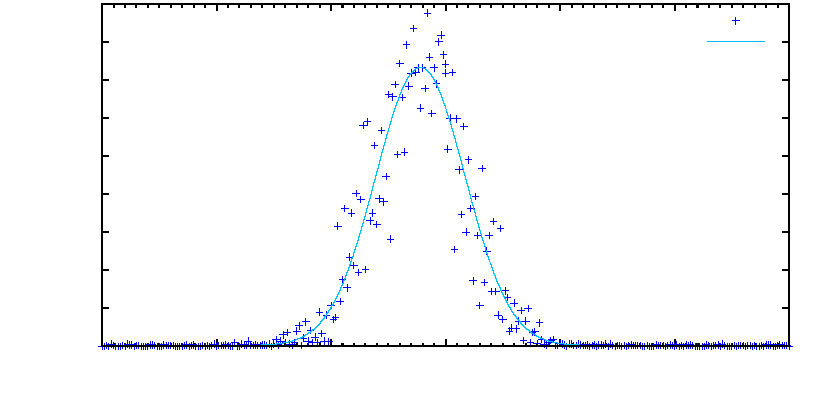
\includegraphics{linienscans_altes_schema_FES}}%
    \gplfronttext
  \end{picture}%
\endgroup

	}
	}}
	\caption[Anregungsschritte, altes System]{Linien aller drei Übergänge des
	alten Schemas.}
	\label{fig:linienscans_altes_schema}
\end{figure}
Die jeweiligen Anpassungsfunktionen finden sich an den einzelnen Plots. Erste
und zweite Schritte werden mit Gaußprofilen angepasst. Für
AI-Linien wird - sofern nicht anders sinnvoller - ein Fano-Profil angenommen.
Die angegebenen Wellenlängen in den Bildüberschriften beziehen sich auf die
Relativfrequenz "'$0$"'. Daten von
Plots mit Relativfrequenzen wurden automatisch aufgenommen. Im Falle der
manuellen Aufnahme mit dem Wavemeter sind Absolutfrequenzen angegeben. Der
jeweilige Fehler der Wellenlänge setzt sich aus der Unsicherheiten der
Peaklage des Fits und der Ungenauigkeit des Wavemeters
($40\,$MHz, systematisch) zusammen.
Der Fehler des jeweiligen Energieniveaus setzt sich aus allen
Peaklage-Unsicherheiten der zur Besetzung verwendeten Übergänge und dem
systematischen Fehler des Wavemeters zusammen.
Die sehr schmalen Linienbreiten erlauben isotopenselektive Ionisation mit eine Selektivität von
$2,5\cdot10^7$, was in \cite{raeder:2011:dissertation} gezeigt wurde. Ziel ist
es, ein ähnlich selektives und effizientes Schema mit dem neuen,
zukunftsorientierteren Lasersystem zu finden.

\subsection{Suche nach neuen Anregungsschemata}\label{subsec:schema_suche}
Für die Suche der neuen Anregungsschemata wurde das alte System parallel als
Referenzsystem verwendet, um Vergleiche zu anderen Anregungsleitern ziehen
zu können. Als Grundlage neuer Schemata dient die Arbeit
\cite{raeder:2011:dissertation}, aus der einige Spektren zweiter und dritter
Anregungsschritte entnommen wurden, die von verschiedenen FES ausgehen. Hierbei
bieten sich drei erste Schritte an, die mit dem blauen $405\,$nm-Diodenlaser aus dem neuen System erreicht werden können. Dabei wird allerdings nicht vom GZ, sondern von einem thermisch angeregten
Zustand ausgegangen ($620,323\,$cm$^{-1}$ über dem GZ). Die als
Grundlage dienenden Spektren wurden in Mainz mit gepulst betriebenen
Ti:Sa-Lasern aufgenommen. Die FES liegen bei $25235,7\,$cm$^{-1}$,
$25319,3\,$cm$^{-1}$ und $25349,0\,$cm$^{-1}$, welche Übergangswellenlängen von $406,25\,$nm, $404,88\,$nm und $404,39\,$nm
entsprechen. Die im Rahmen dieser Arbeit durchgeführten Untersuchungen mit
cw-Diodenlasern beschränken sich bis zum Zeitpunkt der Abgabe dieser Arbeit auf
die ersten Schritte mit $404,88\,$nm und $404,39\,$nm und sollen im Folgenden genauer
betrachtet werden.\par
\begin{figure}[h]
 	\centering
 	\fbox{\parbox{\dimexpr \linewidth - 2\fboxrule - 2\fboxsep}{
 	\centering
	    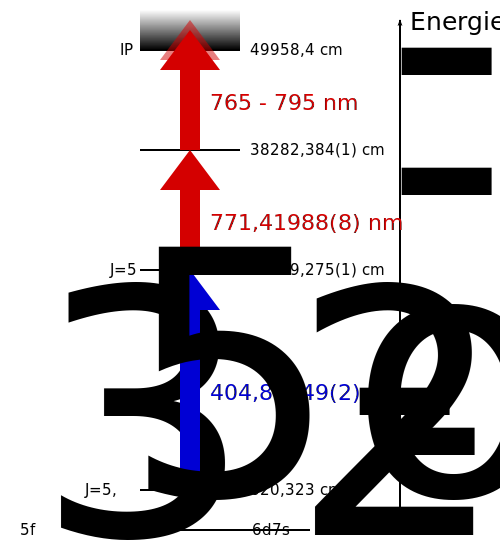
\includegraphics[width=\textwidth-7cm]{gfx/anregungsschema_neu_01}
	    }}
	\caption[Anregungsschema, neu (1)]{Erstes Anregungsschema des neuen
	Systems.}
	\label{fig:anregungsschema_neu_01}
\end{figure}
Nach den Untersuchungen aus \cite{raeder:2011:dissertation} bietet sich das in
Abb. \ref{fig:anregungsschema_neu_01} dargestellte Anregungsschema aufrund der
Erreichbarkeit mit den Lasern des neuen Systems an. Da die bisher
aufgenommenen AI-Spektren dieses Schemas breitbandig und mit niedriger Auflösung vorliegen, war es nötig eine Auswahl von
interessanten AIs (schmal und intensiv) im mit dem \textit{TA-Pro} erreichbaren
Bereich von $765$ bis $795\,$nm vorzunehmen. Es stellte
sich heraus, dass es sich bei den untersuchten AIs ausschließlich um mehrere GHz
breite Strukturen handelt, die sich nicht für HR-RIMS eignen, wie das Beispiel
in Abb. \ref{fig:linienscans_neues_schema_01_AI_bsp} zeigt.
\begin{figure}[h]
 	\centering
 	\footnotesize
	% GNUPLOT: LaTeX picture with Postscript
\begingroup
  \makeatletter
  \providecommand\color[2][]{%
    \GenericError{(gnuplot) \space\space\space\@spaces}{%
      Package color not loaded in conjunction with
      terminal option `colourtext'%
    }{See the gnuplot documentation for explanation.%
    }{Either use 'blacktext' in gnuplot or load the package
      color.sty in LaTeX.}%
    \renewcommand\color[2][]{}%
  }%
  \providecommand\includegraphics[2][]{%
    \GenericError{(gnuplot) \space\space\space\@spaces}{%
      Package graphicx or graphics not loaded%
    }{See the gnuplot documentation for explanation.%
    }{The gnuplot epslatex terminal needs graphicx.sty or graphics.sty.}%
    \renewcommand\includegraphics[2][]{}%
  }%
  \providecommand\rotatebox[2]{#2}%
  \@ifundefined{ifGPcolor}{%
    \newif\ifGPcolor
    \GPcolortrue
  }{}%
  \@ifundefined{ifGPblacktext}{%
    \newif\ifGPblacktext
    \GPblacktexttrue
  }{}%
  % define a \g@addto@macro without @ in the name:
  \let\gplgaddtomacro\g@addto@macro
  % define empty templates for all commands taking text:
  \gdef\gplbacktext{}%
  \gdef\gplfronttext{}%
  \makeatother
  \ifGPblacktext
    % no textcolor at all
    \def\colorrgb#1{}%
    \def\colorgray#1{}%
  \else
    % gray or color?
    \ifGPcolor
      \def\colorrgb#1{\color[rgb]{#1}}%
      \def\colorgray#1{\color[gray]{#1}}%
      \expandafter\def\csname LTw\endcsname{\color{white}}%
      \expandafter\def\csname LTb\endcsname{\color{black}}%
      \expandafter\def\csname LTa\endcsname{\color{black}}%
      \expandafter\def\csname LT0\endcsname{\color[rgb]{1,0,0}}%
      \expandafter\def\csname LT1\endcsname{\color[rgb]{0,1,0}}%
      \expandafter\def\csname LT2\endcsname{\color[rgb]{0,0,1}}%
      \expandafter\def\csname LT3\endcsname{\color[rgb]{1,0,1}}%
      \expandafter\def\csname LT4\endcsname{\color[rgb]{0,1,1}}%
      \expandafter\def\csname LT5\endcsname{\color[rgb]{1,1,0}}%
      \expandafter\def\csname LT6\endcsname{\color[rgb]{0,0,0}}%
      \expandafter\def\csname LT7\endcsname{\color[rgb]{1,0.3,0}}%
      \expandafter\def\csname LT8\endcsname{\color[rgb]{0.5,0.5,0.5}}%
    \else
      % gray
      \def\colorrgb#1{\color{black}}%
      \def\colorgray#1{\color[gray]{#1}}%
      \expandafter\def\csname LTw\endcsname{\color{white}}%
      \expandafter\def\csname LTb\endcsname{\color{black}}%
      \expandafter\def\csname LTa\endcsname{\color{black}}%
      \expandafter\def\csname LT0\endcsname{\color{black}}%
      \expandafter\def\csname LT1\endcsname{\color{black}}%
      \expandafter\def\csname LT2\endcsname{\color{black}}%
      \expandafter\def\csname LT3\endcsname{\color{black}}%
      \expandafter\def\csname LT4\endcsname{\color{black}}%
      \expandafter\def\csname LT5\endcsname{\color{black}}%
      \expandafter\def\csname LT6\endcsname{\color{black}}%
      \expandafter\def\csname LT7\endcsname{\color{black}}%
      \expandafter\def\csname LT8\endcsname{\color{black}}%
    \fi
  \fi
  \setlength{\unitlength}{0.0500bp}%
  \begin{picture}(7936.00,3968.00)%
    \gplgaddtomacro\gplbacktext{%
      \csname LTb\endcsname%
      \put(980,640){\makebox(0,0)[r]{\strut{} 1000}}%
      \put(980,1297){\makebox(0,0)[r]{\strut{} 2000}}%
      \put(980,1955){\makebox(0,0)[r]{\strut{} 3000}}%
      \put(980,2612){\makebox(0,0)[r]{\strut{} 4000}}%
      \put(980,3270){\makebox(0,0)[r]{\strut{} 5000}}%
      \put(980,3927){\makebox(0,0)[r]{\strut{} 6000}}%
      \put(1100,440){\makebox(0,0){\strut{}387.884}}%
      \put(2395,440){\makebox(0,0){\strut{}387.888}}%
      \put(3690,440){\makebox(0,0){\strut{}387.892}}%
      \put(4985,440){\makebox(0,0){\strut{}387.896}}%
      \put(6280,440){\makebox(0,0){\strut{}387.900}}%
      \put(7575,440){\makebox(0,0){\strut{}387.904}}%
      \put(160,2283){\rotatebox{-270}{\makebox(0,0){\strut{}Countrate [s$^{-1}$]}}}%
      \put(4337,140){\makebox(0,0){\strut{}Frequenz [THz]}}%
      \put(3366,2119){\makebox(0,0)[l]{\strut{}$G(\nu)=A\cdot\frac{1}{\sigma\sqrt{2\pi}}\mathrm{e}^{-\frac{1}{2}\frac{(\nu-\mu)^2}{\sigma^2}}+b$}}%
      \put(3366,1626){\makebox(0,0)[l]{\strut{}$2\sigma = (10.59\pm0.54)\,$GHz}}%
      \put(3366,1396){\makebox(0,0)[l]{\strut{}$\mu = (387.895592\pm0.000068)\,$THz}}%
      \put(3366,1166){\makebox(0,0)[l]{\strut{}$A = (38.5\pm4.0)\,\nicefrac{\text{MHz}}{\text{s}}$}}%
      \put(3366,936){\makebox(0,0)[l]{\strut{}$b = (2039\pm168)\,$s$^{-1}$}}%
    }%
    \gplgaddtomacro\gplfronttext{%
      \csname LTb\endcsname%
      \put(6672,3764){\makebox(0,0)[r]{\strut{}Messpunkte}}%
      \csname LTb\endcsname%
      \put(6672,3564){\makebox(0,0)[r]{\strut{}Fit}}%
    }%
    \gplbacktext
    \put(0,0){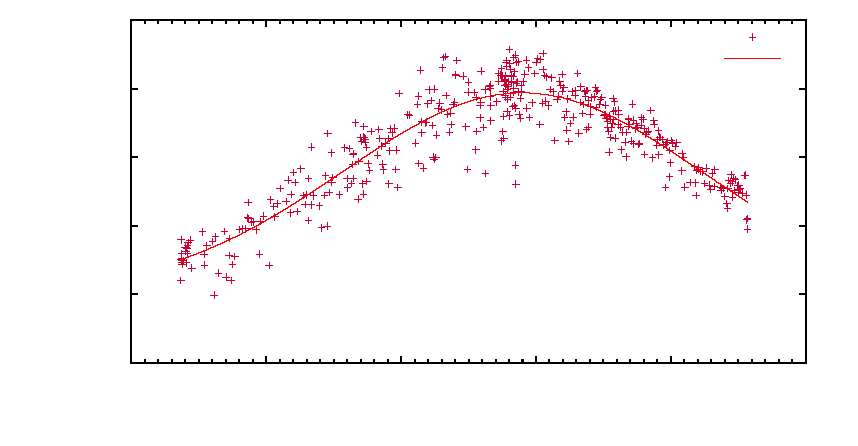
\includegraphics{linienscans_neues_schema_01_AI_bsp_mean}}%
    \gplfronttext
  \end{picture}%
\endgroup

	\caption[AI Beispiel, neues Schema (1)]{Beispiel eines sehr breiten AIs aus dem
	Anregungsschema in Abb. \ref{fig:anregungsschema_neu_01}. Die
	Zentralwellenlänge liegt bei $772,8690(2)\,$nm}.
	\label{fig:linienscans_neues_schema_01_AI_bsp}
\end{figure}
Im Zentrum einer dieser AIs wurden für die ersten beiden Anregungsschritte
Linienprofile aufgenommen, welche sich in Abb. \ref{fig:linienscans_neues_schema_01} finden.
\begin{figure}[hp]
 	\centering
 	\footnotesize
 	\fbox{\parbox{\dimexpr \linewidth - 2\fboxrule - 2\fboxsep}{
 	\subfloat[Zweiter Anregungsschritt @ $771,41988(8)\,$nm]{
		\label{subfig:linienscans_neues_schema_01_SES}
		% GNUPLOT: LaTeX picture with Postscript
\begingroup
  \makeatletter
  \providecommand\color[2][]{%
    \GenericError{(gnuplot) \space\space\space\@spaces}{%
      Package color not loaded in conjunction with
      terminal option `colourtext'%
    }{See the gnuplot documentation for explanation.%
    }{Either use 'blacktext' in gnuplot or load the package
      color.sty in LaTeX.}%
    \renewcommand\color[2][]{}%
  }%
  \providecommand\includegraphics[2][]{%
    \GenericError{(gnuplot) \space\space\space\@spaces}{%
      Package graphicx or graphics not loaded%
    }{See the gnuplot documentation for explanation.%
    }{The gnuplot epslatex terminal needs graphicx.sty or graphics.sty.}%
    \renewcommand\includegraphics[2][]{}%
  }%
  \providecommand\rotatebox[2]{#2}%
  \@ifundefined{ifGPcolor}{%
    \newif\ifGPcolor
    \GPcolortrue
  }{}%
  \@ifundefined{ifGPblacktext}{%
    \newif\ifGPblacktext
    \GPblacktexttrue
  }{}%
  % define a \g@addto@macro without @ in the name:
  \let\gplgaddtomacro\g@addto@macro
  % define empty templates for all commands taking text:
  \gdef\gplbacktext{}%
  \gdef\gplfronttext{}%
  \makeatother
  \ifGPblacktext
    % no textcolor at all
    \def\colorrgb#1{}%
    \def\colorgray#1{}%
  \else
    % gray or color?
    \ifGPcolor
      \def\colorrgb#1{\color[rgb]{#1}}%
      \def\colorgray#1{\color[gray]{#1}}%
      \expandafter\def\csname LTw\endcsname{\color{white}}%
      \expandafter\def\csname LTb\endcsname{\color{black}}%
      \expandafter\def\csname LTa\endcsname{\color{black}}%
      \expandafter\def\csname LT0\endcsname{\color[rgb]{1,0,0}}%
      \expandafter\def\csname LT1\endcsname{\color[rgb]{0,1,0}}%
      \expandafter\def\csname LT2\endcsname{\color[rgb]{0,0,1}}%
      \expandafter\def\csname LT3\endcsname{\color[rgb]{1,0,1}}%
      \expandafter\def\csname LT4\endcsname{\color[rgb]{0,1,1}}%
      \expandafter\def\csname LT5\endcsname{\color[rgb]{1,1,0}}%
      \expandafter\def\csname LT6\endcsname{\color[rgb]{0,0,0}}%
      \expandafter\def\csname LT7\endcsname{\color[rgb]{1,0.3,0}}%
      \expandafter\def\csname LT8\endcsname{\color[rgb]{0.5,0.5,0.5}}%
    \else
      % gray
      \def\colorrgb#1{\color{black}}%
      \def\colorgray#1{\color[gray]{#1}}%
      \expandafter\def\csname LTw\endcsname{\color{white}}%
      \expandafter\def\csname LTb\endcsname{\color{black}}%
      \expandafter\def\csname LTa\endcsname{\color{black}}%
      \expandafter\def\csname LT0\endcsname{\color{black}}%
      \expandafter\def\csname LT1\endcsname{\color{black}}%
      \expandafter\def\csname LT2\endcsname{\color{black}}%
      \expandafter\def\csname LT3\endcsname{\color{black}}%
      \expandafter\def\csname LT4\endcsname{\color{black}}%
      \expandafter\def\csname LT5\endcsname{\color{black}}%
      \expandafter\def\csname LT6\endcsname{\color{black}}%
      \expandafter\def\csname LT7\endcsname{\color{black}}%
      \expandafter\def\csname LT8\endcsname{\color{black}}%
    \fi
  \fi
  \setlength{\unitlength}{0.0500bp}%
  \begin{picture}(7936.00,3968.00)%
    \gplgaddtomacro\gplbacktext{%
      \csname LTb\endcsname%
      \put(860,640){\makebox(0,0)[r]{\strut{} 0}}%
      \put(860,1051){\makebox(0,0)[r]{\strut{} 100}}%
      \put(860,1462){\makebox(0,0)[r]{\strut{} 200}}%
      \put(860,1873){\makebox(0,0)[r]{\strut{} 300}}%
      \put(860,2283){\makebox(0,0)[r]{\strut{} 400}}%
      \put(860,2694){\makebox(0,0)[r]{\strut{} 500}}%
      \put(860,3105){\makebox(0,0)[r]{\strut{} 600}}%
      \put(860,3516){\makebox(0,0)[r]{\strut{} 700}}%
      \put(860,3927){\makebox(0,0)[r]{\strut{} 800}}%
      \put(980,440){\makebox(0,0){\strut{}-200}}%
      \put(1804,440){\makebox(0,0){\strut{}-150}}%
      \put(2629,440){\makebox(0,0){\strut{}-100}}%
      \put(3453,440){\makebox(0,0){\strut{}-50}}%
      \put(4278,440){\makebox(0,0){\strut{} 0}}%
      \put(5102,440){\makebox(0,0){\strut{} 50}}%
      \put(5926,440){\makebox(0,0){\strut{} 100}}%
      \put(6751,440){\makebox(0,0){\strut{} 150}}%
      \put(7575,440){\makebox(0,0){\strut{} 200}}%
      \put(160,2283){\rotatebox{-270}{\makebox(0,0){\strut{}Countrate [s$^{-1}$]}}}%
      \put(4277,140){\makebox(0,0){\strut{}Relativfrequenz [MHz]}}%
      \put(1178,3598){\makebox(0,0)[l]{\strut{}$G(\nu)=A\cdot\frac{1}{\sigma\sqrt{2\pi}}\mathrm{e}^{-\frac{1}{2}\frac{(\nu-\mu)^2}{\sigma^2}}+b$}}%
      \put(1178,3105){\makebox(0,0)[l]{\strut{}$2\sigma = (18.49\pm0.20)\,$MHz}}%
      \put(1178,2875){\makebox(0,0)[l]{\strut{}$\mu = (17.13\pm0.10)\,$MHz}}%
      \put(1178,2645){\makebox(0,0)[l]{\strut{}$A = (16391\pm158)\,\nicefrac{\text{MHz}}{\text{s}}$}}%
      \put(1178,2415){\makebox(0,0)[l]{\strut{}$b = (15.4\pm1.1)\,$s$^{-1}$}}%
    }%
    \gplgaddtomacro\gplfronttext{%
      \csname LTb\endcsname%
      \put(6672,3764){\makebox(0,0)[r]{\strut{}Messpunkte}}%
      \csname LTb\endcsname%
      \put(6672,3564){\makebox(0,0)[r]{\strut{}Fit}}%
    }%
    \gplbacktext
    \put(0,0){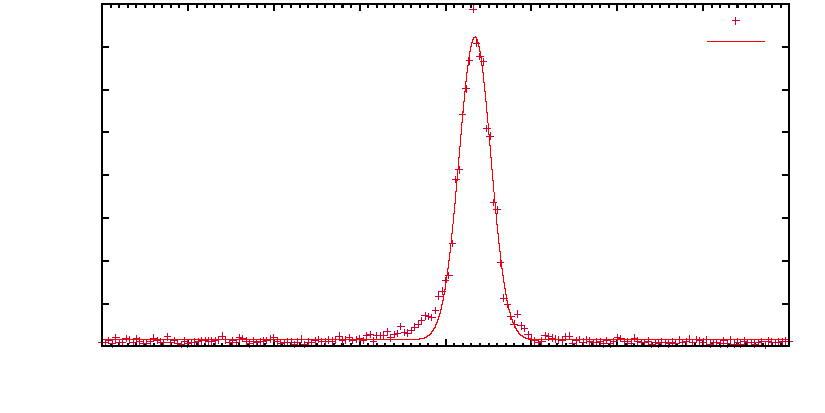
\includegraphics{linienscans_neues_schema_01_SES}}%
    \gplfronttext
  \end{picture}%
\endgroup

	}\\
	\subfloat[Erster Anregungsschritt @ $404,87549(2)\,$nm]{
		\label{subfig:linienscans_neues_schema_01_FES}
		% GNUPLOT: LaTeX picture with Postscript
\begingroup
  \makeatletter
  \providecommand\color[2][]{%
    \GenericError{(gnuplot) \space\space\space\@spaces}{%
      Package color not loaded in conjunction with
      terminal option `colourtext'%
    }{See the gnuplot documentation for explanation.%
    }{Either use 'blacktext' in gnuplot or load the package
      color.sty in LaTeX.}%
    \renewcommand\color[2][]{}%
  }%
  \providecommand\includegraphics[2][]{%
    \GenericError{(gnuplot) \space\space\space\@spaces}{%
      Package graphicx or graphics not loaded%
    }{See the gnuplot documentation for explanation.%
    }{The gnuplot epslatex terminal needs graphicx.sty or graphics.sty.}%
    \renewcommand\includegraphics[2][]{}%
  }%
  \providecommand\rotatebox[2]{#2}%
  \@ifundefined{ifGPcolor}{%
    \newif\ifGPcolor
    \GPcolortrue
  }{}%
  \@ifundefined{ifGPblacktext}{%
    \newif\ifGPblacktext
    \GPblacktexttrue
  }{}%
  % define a \g@addto@macro without @ in the name:
  \let\gplgaddtomacro\g@addto@macro
  % define empty templates for all commands taking text:
  \gdef\gplbacktext{}%
  \gdef\gplfronttext{}%
  \makeatother
  \ifGPblacktext
    % no textcolor at all
    \def\colorrgb#1{}%
    \def\colorgray#1{}%
  \else
    % gray or color?
    \ifGPcolor
      \def\colorrgb#1{\color[rgb]{#1}}%
      \def\colorgray#1{\color[gray]{#1}}%
      \expandafter\def\csname LTw\endcsname{\color{white}}%
      \expandafter\def\csname LTb\endcsname{\color{black}}%
      \expandafter\def\csname LTa\endcsname{\color{black}}%
      \expandafter\def\csname LT0\endcsname{\color[rgb]{1,0,0}}%
      \expandafter\def\csname LT1\endcsname{\color[rgb]{0,1,0}}%
      \expandafter\def\csname LT2\endcsname{\color[rgb]{0,0,1}}%
      \expandafter\def\csname LT3\endcsname{\color[rgb]{1,0,1}}%
      \expandafter\def\csname LT4\endcsname{\color[rgb]{0,1,1}}%
      \expandafter\def\csname LT5\endcsname{\color[rgb]{1,1,0}}%
      \expandafter\def\csname LT6\endcsname{\color[rgb]{0,0,0}}%
      \expandafter\def\csname LT7\endcsname{\color[rgb]{1,0.3,0}}%
      \expandafter\def\csname LT8\endcsname{\color[rgb]{0.5,0.5,0.5}}%
    \else
      % gray
      \def\colorrgb#1{\color{black}}%
      \def\colorgray#1{\color[gray]{#1}}%
      \expandafter\def\csname LTw\endcsname{\color{white}}%
      \expandafter\def\csname LTb\endcsname{\color{black}}%
      \expandafter\def\csname LTa\endcsname{\color{black}}%
      \expandafter\def\csname LT0\endcsname{\color{black}}%
      \expandafter\def\csname LT1\endcsname{\color{black}}%
      \expandafter\def\csname LT2\endcsname{\color{black}}%
      \expandafter\def\csname LT3\endcsname{\color{black}}%
      \expandafter\def\csname LT4\endcsname{\color{black}}%
      \expandafter\def\csname LT5\endcsname{\color{black}}%
      \expandafter\def\csname LT6\endcsname{\color{black}}%
      \expandafter\def\csname LT7\endcsname{\color{black}}%
      \expandafter\def\csname LT8\endcsname{\color{black}}%
    \fi
  \fi
  \setlength{\unitlength}{0.0500bp}%
  \begin{picture}(7936.00,3968.00)%
    \gplgaddtomacro\gplbacktext{%
      \csname LTb\endcsname%
      \put(860,640){\makebox(0,0)[r]{\strut{} 0}}%
      \put(860,969){\makebox(0,0)[r]{\strut{} 20}}%
      \put(860,1297){\makebox(0,0)[r]{\strut{} 40}}%
      \put(860,1626){\makebox(0,0)[r]{\strut{} 60}}%
      \put(860,1955){\makebox(0,0)[r]{\strut{} 80}}%
      \put(860,2283){\makebox(0,0)[r]{\strut{} 100}}%
      \put(860,2612){\makebox(0,0)[r]{\strut{} 120}}%
      \put(860,2941){\makebox(0,0)[r]{\strut{} 140}}%
      \put(860,3270){\makebox(0,0)[r]{\strut{} 160}}%
      \put(860,3598){\makebox(0,0)[r]{\strut{} 180}}%
      \put(860,3927){\makebox(0,0)[r]{\strut{} 200}}%
      \put(980,440){\makebox(0,0){\strut{}-600}}%
      \put(2079,440){\makebox(0,0){\strut{}-400}}%
      \put(3178,440){\makebox(0,0){\strut{}-200}}%
      \put(4278,440){\makebox(0,0){\strut{} 0}}%
      \put(5377,440){\makebox(0,0){\strut{} 200}}%
      \put(6476,440){\makebox(0,0){\strut{} 400}}%
      \put(7575,440){\makebox(0,0){\strut{} 600}}%
      \put(160,2283){\rotatebox{-270}{\makebox(0,0){\strut{}Countrate [s$^{-1}$]}}}%
      \put(4277,140){\makebox(0,0){\strut{}Relativfrequenz [MHz]}}%
      \put(1178,3598){\makebox(0,0)[l]{\strut{}$G(\nu)=A\cdot\frac{1}{\sigma\sqrt{2\pi}}\mathrm{e}^{-\frac{1}{2}\frac{(\nu-\mu)^2}{\sigma^2}}+b$}}%
      \put(1178,3105){\makebox(0,0)[l]{\strut{}$2\sigma = (107.00\pm1.69)\,$MHz}}%
      \put(1178,2875){\makebox(0,0)[l]{\strut{}$\mu = (96.61\pm0.79)\,$MHz}}%
      \put(1178,2645){\makebox(0,0)[l]{\strut{}$A = (22425\pm339)\,\nicefrac{\text{MHz}}{\text{s}}$}}%
      \put(1178,2415){\makebox(0,0)[l]{\strut{}$b = (3.65\pm0.63)\,$s$^{-1}$}}%
    }%
    \gplgaddtomacro\gplfronttext{%
      \csname LTb\endcsname%
      \put(6672,3764){\makebox(0,0)[r]{\strut{}Messpunkte}}%
      \csname LTb\endcsname%
      \put(6672,3564){\makebox(0,0)[r]{\strut{}Fit}}%
    }%
    \gplbacktext
    \put(0,0){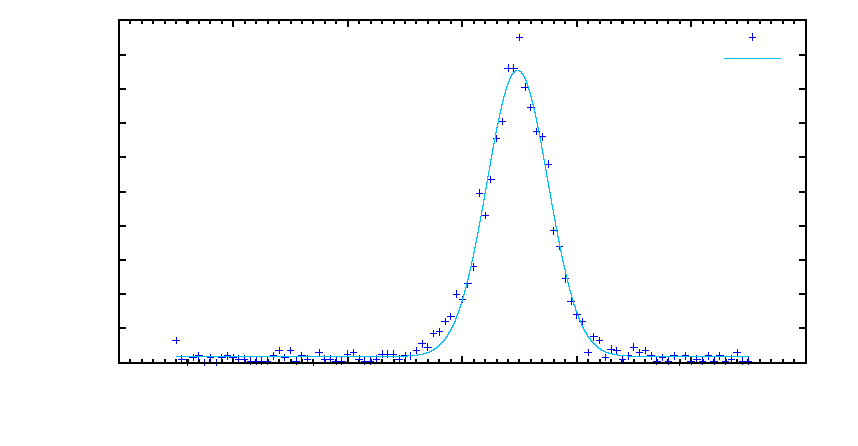
\includegraphics{linienscans_neues_schema_01_FES}}%
    \gplfronttext
  \end{picture}%
\endgroup

	}
	}}
	\caption[erster und zweiter Anregungsschritt, neues System, Schema (1)]{Linien
	der ersten beiden Übergänge des in \ref{fig:anregungsschema_neu_01} gezeigten
	Anregungsschemas.}
	\label{fig:linienscans_neues_schema_01}
\end{figure}
Weiterhin wurde festgestellt, dass sich unter den in
\cite{raeder:2011:dissertation} verzeichneten AI-Spektren Resonanzpeaks
alternativer zweiter Anregungsschritte befinden, da der für den
zweiten Anregungsschritt eingesetzte Laser keinen Einfluss auf das Ionensignal
mehr hatte.
Dabei besetzt der dritte Laser die neu gefundenen SES und
ionisiert gleichzeitig nichtresonant nach. Somit wurden also stichprobenartig
einige vermeintliche AIs als zweite Schritte identifiziert.\par
In diesem Rahmen wurde auch ein signifikant herausstechender zweiter Schritt
gefunden, mit dem $\nicefrac{1}{5}$ der Ionisationsrate des alten Systems mit
nichtresonanter Nachionisation auf gleicher Wellenlänge erreicht wird. Abbildung
\ref{fig:linienscans_neues_schema_01_fake_AI_krass_mean} zeigt das Profil dieses
Anregungsschritts.
\begin{figure}[h]
 	\centering
 	\footnotesize
	% GNUPLOT: LaTeX picture with Postscript
\begingroup
  \makeatletter
  \providecommand\color[2][]{%
    \GenericError{(gnuplot) \space\space\space\@spaces}{%
      Package color not loaded in conjunction with
      terminal option `colourtext'%
    }{See the gnuplot documentation for explanation.%
    }{Either use 'blacktext' in gnuplot or load the package
      color.sty in LaTeX.}%
    \renewcommand\color[2][]{}%
  }%
  \providecommand\includegraphics[2][]{%
    \GenericError{(gnuplot) \space\space\space\@spaces}{%
      Package graphicx or graphics not loaded%
    }{See the gnuplot documentation for explanation.%
    }{The gnuplot epslatex terminal needs graphicx.sty or graphics.sty.}%
    \renewcommand\includegraphics[2][]{}%
  }%
  \providecommand\rotatebox[2]{#2}%
  \@ifundefined{ifGPcolor}{%
    \newif\ifGPcolor
    \GPcolortrue
  }{}%
  \@ifundefined{ifGPblacktext}{%
    \newif\ifGPblacktext
    \GPblacktexttrue
  }{}%
  % define a \g@addto@macro without @ in the name:
  \let\gplgaddtomacro\g@addto@macro
  % define empty templates for all commands taking text:
  \gdef\gplbacktext{}%
  \gdef\gplfronttext{}%
  \makeatother
  \ifGPblacktext
    % no textcolor at all
    \def\colorrgb#1{}%
    \def\colorgray#1{}%
  \else
    % gray or color?
    \ifGPcolor
      \def\colorrgb#1{\color[rgb]{#1}}%
      \def\colorgray#1{\color[gray]{#1}}%
      \expandafter\def\csname LTw\endcsname{\color{white}}%
      \expandafter\def\csname LTb\endcsname{\color{black}}%
      \expandafter\def\csname LTa\endcsname{\color{black}}%
      \expandafter\def\csname LT0\endcsname{\color[rgb]{1,0,0}}%
      \expandafter\def\csname LT1\endcsname{\color[rgb]{0,1,0}}%
      \expandafter\def\csname LT2\endcsname{\color[rgb]{0,0,1}}%
      \expandafter\def\csname LT3\endcsname{\color[rgb]{1,0,1}}%
      \expandafter\def\csname LT4\endcsname{\color[rgb]{0,1,1}}%
      \expandafter\def\csname LT5\endcsname{\color[rgb]{1,1,0}}%
      \expandafter\def\csname LT6\endcsname{\color[rgb]{0,0,0}}%
      \expandafter\def\csname LT7\endcsname{\color[rgb]{1,0.3,0}}%
      \expandafter\def\csname LT8\endcsname{\color[rgb]{0.5,0.5,0.5}}%
    \else
      % gray
      \def\colorrgb#1{\color{black}}%
      \def\colorgray#1{\color[gray]{#1}}%
      \expandafter\def\csname LTw\endcsname{\color{white}}%
      \expandafter\def\csname LTb\endcsname{\color{black}}%
      \expandafter\def\csname LTa\endcsname{\color{black}}%
      \expandafter\def\csname LT0\endcsname{\color{black}}%
      \expandafter\def\csname LT1\endcsname{\color{black}}%
      \expandafter\def\csname LT2\endcsname{\color{black}}%
      \expandafter\def\csname LT3\endcsname{\color{black}}%
      \expandafter\def\csname LT4\endcsname{\color{black}}%
      \expandafter\def\csname LT5\endcsname{\color{black}}%
      \expandafter\def\csname LT6\endcsname{\color{black}}%
      \expandafter\def\csname LT7\endcsname{\color{black}}%
      \expandafter\def\csname LT8\endcsname{\color{black}}%
    \fi
  \fi
  \setlength{\unitlength}{0.0500bp}%
  \begin{picture}(7936.00,3968.00)%
    \gplgaddtomacro\gplbacktext{%
      \csname LTb\endcsname%
      \put(1100,640){\makebox(0,0)[r]{\strut{} 0}}%
      \put(1100,969){\makebox(0,0)[r]{\strut{} 1000}}%
      \put(1100,1297){\makebox(0,0)[r]{\strut{} 2000}}%
      \put(1100,1626){\makebox(0,0)[r]{\strut{} 3000}}%
      \put(1100,1955){\makebox(0,0)[r]{\strut{} 4000}}%
      \put(1100,2283){\makebox(0,0)[r]{\strut{} 5000}}%
      \put(1100,2612){\makebox(0,0)[r]{\strut{} 6000}}%
      \put(1100,2941){\makebox(0,0)[r]{\strut{} 7000}}%
      \put(1100,3270){\makebox(0,0)[r]{\strut{} 8000}}%
      \put(1100,3598){\makebox(0,0)[r]{\strut{} 9000}}%
      \put(1100,3927){\makebox(0,0)[r]{\strut{} 10000}}%
      \put(2179,440){\makebox(0,0){\strut{}385.263100}}%
      \put(3378,440){\makebox(0,0){\strut{}385.263150}}%
      \put(4577,440){\makebox(0,0){\strut{}385.263200}}%
      \put(5776,440){\makebox(0,0){\strut{}385.263250}}%
      \put(6975,440){\makebox(0,0){\strut{}385.263300}}%
      \put(160,2283){\rotatebox{-270}{\makebox(0,0){\strut{}Countrate [s$^{-1}$]}}}%
      \put(4397,140){\makebox(0,0){\strut{}Frequenz [THz]}}%
      \put(4080,2809){\makebox(0,0)[l]{\strut{}$G(\nu)=A\cdot\frac{1}{\sigma\sqrt{2\pi}}\mathrm{e}^{-\frac{1}{2}\frac{(\nu-\mu)^2}{\sigma^2}}+b$}}%
      \put(4080,2316){\makebox(0,0)[l]{\strut{}$2\sigma = (28.65\pm0.54)\,$MHz}}%
      \put(4080,2086){\makebox(0,0)[l]{\strut{}$\mu = (385.26314326\pm0.00000021)\,$THz}}%
      \put(4080,1856){\makebox(0,0)[l]{\strut{}$A = (0.3121\pm0.0066)\,\nicefrac{\text{MHz}}{\text{s}}$}}%
      \put(4080,1626){\makebox(0,0)[l]{\strut{}$b = (543\pm66)\,$s$^{-1}$}}%
    }%
    \gplgaddtomacro\gplfronttext{%
      \csname LTb\endcsname%
      \put(6672,3764){\makebox(0,0)[r]{\strut{}Messpunkte}}%
      \csname LTb\endcsname%
      \put(6672,3564){\makebox(0,0)[r]{\strut{}Fit}}%
    }%
    \gplbacktext
    \put(0,0){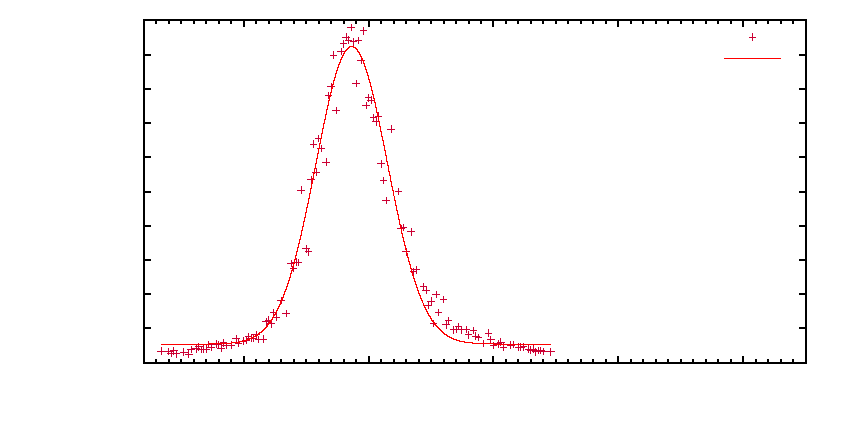
\includegraphics{linienscans_neues_schema_01_fake_AI_krass_mean}}%
    \gplfronttext
  \end{picture}%
\endgroup

	\caption[zweiter Schritt aus AI-Spektren]{Profil eines zweiten
	Anregungsschritts mit nichtresonanter Nachionisation. Dieser Schritt wurde im
	Rahmen der Überprüfung der in \cite{raeder:2011:dissertation} dokumentierten
	AI-Spektren gefunden. Die Zentralwellenlänge liegt bei $778,14986(8)\,$nm.}
	\label{fig:linienscans_neues_schema_01_fake_AI_krass_mean}
\end{figure}
Es wurde getestet, ob die ungewöhnlich hohe, nichtresonante Ionisationsrate für
diesen Schritt durch einen in der Nähe dieser Frequenz liegenden AI verursacht
wird. Dazu wurde der \textit{DL-Pro} auf den gefundenen zweiten Schritt
eingestellt und ein mehrere GHz breiter Scan in der Umgebung mit dem \textit{TA-Pro} durchgeführt.
Das Ergebnis ist in Abb.
\ref{fig:linienscans_neues_schema_01_fake_AI_krass_umgebung_mean} zu sehen.
\begin{figure}[h]
 	\centering
 	\footnotesize
	% GNUPLOT: LaTeX picture with Postscript
\begingroup
  \makeatletter
  \providecommand\color[2][]{%
    \GenericError{(gnuplot) \space\space\space\@spaces}{%
      Package color not loaded in conjunction with
      terminal option `colourtext'%
    }{See the gnuplot documentation for explanation.%
    }{Either use 'blacktext' in gnuplot or load the package
      color.sty in LaTeX.}%
    \renewcommand\color[2][]{}%
  }%
  \providecommand\includegraphics[2][]{%
    \GenericError{(gnuplot) \space\space\space\@spaces}{%
      Package graphicx or graphics not loaded%
    }{See the gnuplot documentation for explanation.%
    }{The gnuplot epslatex terminal needs graphicx.sty or graphics.sty.}%
    \renewcommand\includegraphics[2][]{}%
  }%
  \providecommand\rotatebox[2]{#2}%
  \@ifundefined{ifGPcolor}{%
    \newif\ifGPcolor
    \GPcolortrue
  }{}%
  \@ifundefined{ifGPblacktext}{%
    \newif\ifGPblacktext
    \GPblacktexttrue
  }{}%
  % define a \g@addto@macro without @ in the name:
  \let\gplgaddtomacro\g@addto@macro
  % define empty templates for all commands taking text:
  \gdef\gplbacktext{}%
  \gdef\gplfronttext{}%
  \makeatother
  \ifGPblacktext
    % no textcolor at all
    \def\colorrgb#1{}%
    \def\colorgray#1{}%
  \else
    % gray or color?
    \ifGPcolor
      \def\colorrgb#1{\color[rgb]{#1}}%
      \def\colorgray#1{\color[gray]{#1}}%
      \expandafter\def\csname LTw\endcsname{\color{white}}%
      \expandafter\def\csname LTb\endcsname{\color{black}}%
      \expandafter\def\csname LTa\endcsname{\color{black}}%
      \expandafter\def\csname LT0\endcsname{\color[rgb]{1,0,0}}%
      \expandafter\def\csname LT1\endcsname{\color[rgb]{0,1,0}}%
      \expandafter\def\csname LT2\endcsname{\color[rgb]{0,0,1}}%
      \expandafter\def\csname LT3\endcsname{\color[rgb]{1,0,1}}%
      \expandafter\def\csname LT4\endcsname{\color[rgb]{0,1,1}}%
      \expandafter\def\csname LT5\endcsname{\color[rgb]{1,1,0}}%
      \expandafter\def\csname LT6\endcsname{\color[rgb]{0,0,0}}%
      \expandafter\def\csname LT7\endcsname{\color[rgb]{1,0.3,0}}%
      \expandafter\def\csname LT8\endcsname{\color[rgb]{0.5,0.5,0.5}}%
    \else
      % gray
      \def\colorrgb#1{\color{black}}%
      \def\colorgray#1{\color[gray]{#1}}%
      \expandafter\def\csname LTw\endcsname{\color{white}}%
      \expandafter\def\csname LTb\endcsname{\color{black}}%
      \expandafter\def\csname LTa\endcsname{\color{black}}%
      \expandafter\def\csname LT0\endcsname{\color{black}}%
      \expandafter\def\csname LT1\endcsname{\color{black}}%
      \expandafter\def\csname LT2\endcsname{\color{black}}%
      \expandafter\def\csname LT3\endcsname{\color{black}}%
      \expandafter\def\csname LT4\endcsname{\color{black}}%
      \expandafter\def\csname LT5\endcsname{\color{black}}%
      \expandafter\def\csname LT6\endcsname{\color{black}}%
      \expandafter\def\csname LT7\endcsname{\color{black}}%
      \expandafter\def\csname LT8\endcsname{\color{black}}%
    \fi
  \fi
  \setlength{\unitlength}{0.0500bp}%
  \begin{picture}(7936.00,3968.00)%
    \gplgaddtomacro\gplbacktext{%
      \csname LTb\endcsname%
      \put(1100,640){\makebox(0,0)[r]{\strut{} 0}}%
      \put(1100,1110){\makebox(0,0)[r]{\strut{} 2000}}%
      \put(1100,1579){\makebox(0,0)[r]{\strut{} 4000}}%
      \put(1100,2049){\makebox(0,0)[r]{\strut{} 6000}}%
      \put(1100,2518){\makebox(0,0)[r]{\strut{} 8000}}%
      \put(1100,2988){\makebox(0,0)[r]{\strut{} 10000}}%
      \put(1100,3457){\makebox(0,0)[r]{\strut{} 12000}}%
      \put(1100,3927){\makebox(0,0)[r]{\strut{} 14000}}%
      \put(1220,440){\makebox(0,0){\strut{}385.255}}%
      \put(2128,440){\makebox(0,0){\strut{}385.260}}%
      \put(3036,440){\makebox(0,0){\strut{}385.265}}%
      \put(3944,440){\makebox(0,0){\strut{}385.270}}%
      \put(4851,440){\makebox(0,0){\strut{}385.275}}%
      \put(5759,440){\makebox(0,0){\strut{}385.280}}%
      \put(6667,440){\makebox(0,0){\strut{}385.285}}%
      \put(7575,440){\makebox(0,0){\strut{}385.290}}%
      \put(160,2283){\rotatebox{-270}{\makebox(0,0){\strut{}Countrate [s$^{-1}$]}}}%
      \put(4397,140){\makebox(0,0){\strut{}Frequenz [THz]}}%
    }%
    \gplgaddtomacro\gplfronttext{%
      \csname LTb\endcsname%
      \put(6672,3764){\makebox(0,0)[r]{\strut{}Messpunkte}}%
    }%
    \gplbacktext
    \put(0,0){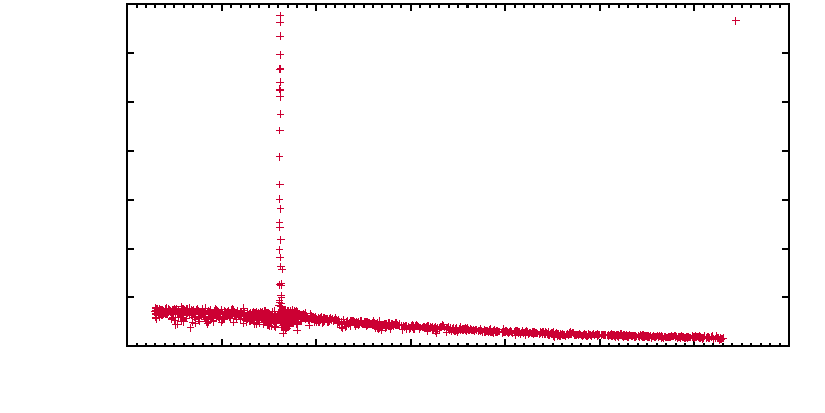
\includegraphics{linienscans_neues_schema_01_fake_AI_krass_umgebung_mean}}%
    \gplfronttext
  \end{picture}%
\endgroup

	\caption[zweiter Schritt aus AI-Spektren, Umgebungsscan]{Mehrere GHz breiten
	AI-Scan in der Frequenzumgebung des neu gefundenen zweiten Schritts aus Abb.
	\ref{fig:linienscans_neues_schema_01_fake_AI_krass_mean}.}
	\label{fig:linienscans_neues_schema_01_fake_AI_krass_umgebung_mean}
\end{figure}
Der Scan zeigt allerdings keinen für die hohe Ionisationrate verantwortlichen AI
in der Umgebung sondern ausschließlich die Resonanzüberhöhung bei
$385,263\,$nm, wenn beide Laser resonant auf dem zweiten Übergang stehen.
Weitere Untersuchungen dieses bisher noch nicht vollständig verstandenen
Phänomens stehen noch an.\par
Es hat sich in der Vergangenheit herausgestellt, dass weit
über dem IP (in diesem Fall $900$ bis $1400\,$cm$^{-1}$) keine
schmalen AI-Strukturen mehr existieren, die sich für HR-RIMS eignen. Wie in
\cite{Bushaw2007485} gezeigt, finden sich aber knapp über dem IP durchaus verwendbare AIs.
Aufgrund dieser Vermutungen wurde ein neues Schema angesetzt
(Abb. \ref{fig:anregungsschema_neu_02}). Dazu wurde für den zweiten
Anregungsschritt ein weiterer Diodenlaser mit $830\,$nm alternativ zum
\textit{DL-Pro} aufgebaut. Die Profile der ersten beiden
Anregungsschritte sind in Abb. \ref{fig:linienscans_neues_schema_02}
dargestellt, wobei zur Ionisation ein AI bei $782,32\,$nm genutzt werden konnte,
zu dem es aber noch keine auswertbare Daten gibt. Abbildung
\ref{fig:linienscans_neues_schema_02_AIs} zeigt einige der zuletzt gemessenen
AIs aus diesem Schema.
\begin{figure}[h]
 	\centering
 	\fbox{\parbox{\dimexpr \linewidth - 2\fboxrule - 2\fboxsep}{
 	\centering
	    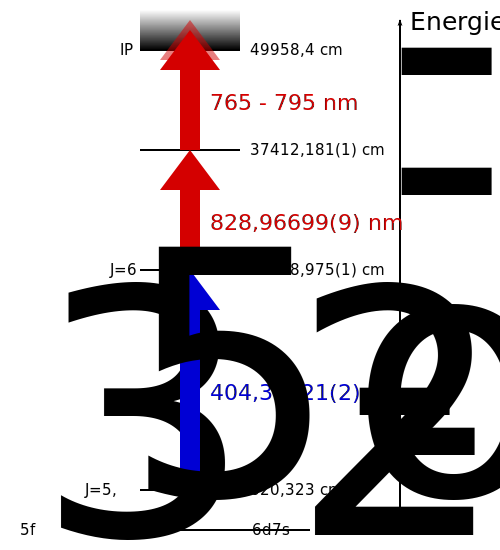
\includegraphics[width=\textwidth-7cm]{gfx/anregungsschema_neu_02}
	    }}
	\caption[Anregungsschema, neu (1)]{Zweites Anregungsschema des neuen
	Systems.}
	\label{fig:anregungsschema_neu_02}
\end{figure}
\begin{figure}[hp]
 	\centering
 	\footnotesize
 	\fbox{\parbox{\dimexpr \linewidth - 2\fboxrule - 2\fboxsep}{
 	\subfloat[Zweiter Anregungsschritt @ $828,96699(9)\,$nm]{
		\label{subfig:linienscans_neues_schema_02_SES_mean}
		% GNUPLOT: LaTeX picture with Postscript
\begingroup
  \makeatletter
  \providecommand\color[2][]{%
    \GenericError{(gnuplot) \space\space\space\@spaces}{%
      Package color not loaded in conjunction with
      terminal option `colourtext'%
    }{See the gnuplot documentation for explanation.%
    }{Either use 'blacktext' in gnuplot or load the package
      color.sty in LaTeX.}%
    \renewcommand\color[2][]{}%
  }%
  \providecommand\includegraphics[2][]{%
    \GenericError{(gnuplot) \space\space\space\@spaces}{%
      Package graphicx or graphics not loaded%
    }{See the gnuplot documentation for explanation.%
    }{The gnuplot epslatex terminal needs graphicx.sty or graphics.sty.}%
    \renewcommand\includegraphics[2][]{}%
  }%
  \providecommand\rotatebox[2]{#2}%
  \@ifundefined{ifGPcolor}{%
    \newif\ifGPcolor
    \GPcolortrue
  }{}%
  \@ifundefined{ifGPblacktext}{%
    \newif\ifGPblacktext
    \GPblacktexttrue
  }{}%
  % define a \g@addto@macro without @ in the name:
  \let\gplgaddtomacro\g@addto@macro
  % define empty templates for all commands taking text:
  \gdef\gplbacktext{}%
  \gdef\gplfronttext{}%
  \makeatother
  \ifGPblacktext
    % no textcolor at all
    \def\colorrgb#1{}%
    \def\colorgray#1{}%
  \else
    % gray or color?
    \ifGPcolor
      \def\colorrgb#1{\color[rgb]{#1}}%
      \def\colorgray#1{\color[gray]{#1}}%
      \expandafter\def\csname LTw\endcsname{\color{white}}%
      \expandafter\def\csname LTb\endcsname{\color{black}}%
      \expandafter\def\csname LTa\endcsname{\color{black}}%
      \expandafter\def\csname LT0\endcsname{\color[rgb]{1,0,0}}%
      \expandafter\def\csname LT1\endcsname{\color[rgb]{0,1,0}}%
      \expandafter\def\csname LT2\endcsname{\color[rgb]{0,0,1}}%
      \expandafter\def\csname LT3\endcsname{\color[rgb]{1,0,1}}%
      \expandafter\def\csname LT4\endcsname{\color[rgb]{0,1,1}}%
      \expandafter\def\csname LT5\endcsname{\color[rgb]{1,1,0}}%
      \expandafter\def\csname LT6\endcsname{\color[rgb]{0,0,0}}%
      \expandafter\def\csname LT7\endcsname{\color[rgb]{1,0.3,0}}%
      \expandafter\def\csname LT8\endcsname{\color[rgb]{0.5,0.5,0.5}}%
    \else
      % gray
      \def\colorrgb#1{\color{black}}%
      \def\colorgray#1{\color[gray]{#1}}%
      \expandafter\def\csname LTw\endcsname{\color{white}}%
      \expandafter\def\csname LTb\endcsname{\color{black}}%
      \expandafter\def\csname LTa\endcsname{\color{black}}%
      \expandafter\def\csname LT0\endcsname{\color{black}}%
      \expandafter\def\csname LT1\endcsname{\color{black}}%
      \expandafter\def\csname LT2\endcsname{\color{black}}%
      \expandafter\def\csname LT3\endcsname{\color{black}}%
      \expandafter\def\csname LT4\endcsname{\color{black}}%
      \expandafter\def\csname LT5\endcsname{\color{black}}%
      \expandafter\def\csname LT6\endcsname{\color{black}}%
      \expandafter\def\csname LT7\endcsname{\color{black}}%
      \expandafter\def\csname LT8\endcsname{\color{black}}%
    \fi
  \fi
  \setlength{\unitlength}{0.0500bp}%
  \begin{picture}(7936.00,3968.00)%
    \gplgaddtomacro\gplbacktext{%
      \csname LTb\endcsname%
      \put(980,640){\makebox(0,0)[r]{\strut{} 0}}%
      \put(980,1005){\makebox(0,0)[r]{\strut{} 200}}%
      \put(980,1370){\makebox(0,0)[r]{\strut{} 400}}%
      \put(980,1736){\makebox(0,0)[r]{\strut{} 600}}%
      \put(980,2101){\makebox(0,0)[r]{\strut{} 800}}%
      \put(980,2466){\makebox(0,0)[r]{\strut{} 1000}}%
      \put(980,2831){\makebox(0,0)[r]{\strut{} 1200}}%
      \put(980,3197){\makebox(0,0)[r]{\strut{} 1400}}%
      \put(980,3562){\makebox(0,0)[r]{\strut{} 1600}}%
      \put(980,3927){\makebox(0,0)[r]{\strut{} 1800}}%
      \put(1100,440){\makebox(0,0){\strut{}361.645650}}%
      \put(2179,440){\makebox(0,0){\strut{}361.645700}}%
      \put(3258,440){\makebox(0,0){\strut{}361.645750}}%
      \put(4337,440){\makebox(0,0){\strut{}361.645800}}%
      \put(5417,440){\makebox(0,0){\strut{}361.645850}}%
      \put(6496,440){\makebox(0,0){\strut{}361.645900}}%
      \put(7575,440){\makebox(0,0){\strut{}361.645950}}%
      \put(160,2283){\rotatebox{-270}{\makebox(0,0){\strut{}Countrate [s$^{-1}$]}}}%
      \put(4337,140){\makebox(0,0){\strut{}Frequenz [THz]}}%
      \put(1294,3598){\makebox(0,0)[l]{\strut{}$G(\nu)=A\cdot\frac{1}{\sigma\sqrt{2\pi}}\mathrm{e}^{-\frac{1}{2}\frac{(\nu-\mu)^2}{\sigma^2}}+b$}}%
      \put(1294,3105){\makebox(0,0)[l]{\strut{}$2\sigma = (26.64\pm0.52)\,$MHz}}%
      \put(1294,2875){\makebox(0,0)[l]{\strut{}$\mu = (361.64583384\pm0.00000022)\,$THz}}%
      \put(1294,2645){\makebox(0,0)[l]{\strut{}$A = (0.0541\pm0.0011)\,\nicefrac{\text{MHz}}{\text{s}}$}}%
      \put(1294,2415){\makebox(0,0)[l]{\strut{}$b = (30.0\pm9.9)\,$s$^{-1}$}}%
    }%
    \gplgaddtomacro\gplfronttext{%
      \csname LTb\endcsname%
      \put(6672,3764){\makebox(0,0)[r]{\strut{}Messpunkte}}%
      \csname LTb\endcsname%
      \put(6672,3564){\makebox(0,0)[r]{\strut{}Fit}}%
    }%
    \gplbacktext
    \put(0,0){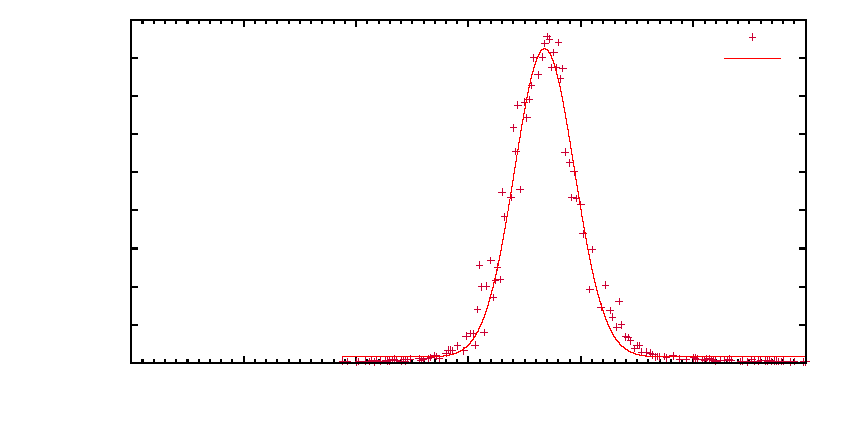
\includegraphics{linienscans_neues_schema_02_SES_mean}}%
    \gplfronttext
  \end{picture}%
\endgroup

	}\\
 	\subfloat[Erster Anregungsschritt @ $404,38921(2)\,$nm]{
		\label{subfig:linienscans_neues_schema_02_FES}
		% GNUPLOT: LaTeX picture with Postscript
\begingroup
  \makeatletter
  \providecommand\color[2][]{%
    \GenericError{(gnuplot) \space\space\space\@spaces}{%
      Package color not loaded in conjunction with
      terminal option `colourtext'%
    }{See the gnuplot documentation for explanation.%
    }{Either use 'blacktext' in gnuplot or load the package
      color.sty in LaTeX.}%
    \renewcommand\color[2][]{}%
  }%
  \providecommand\includegraphics[2][]{%
    \GenericError{(gnuplot) \space\space\space\@spaces}{%
      Package graphicx or graphics not loaded%
    }{See the gnuplot documentation for explanation.%
    }{The gnuplot epslatex terminal needs graphicx.sty or graphics.sty.}%
    \renewcommand\includegraphics[2][]{}%
  }%
  \providecommand\rotatebox[2]{#2}%
  \@ifundefined{ifGPcolor}{%
    \newif\ifGPcolor
    \GPcolortrue
  }{}%
  \@ifundefined{ifGPblacktext}{%
    \newif\ifGPblacktext
    \GPblacktexttrue
  }{}%
  % define a \g@addto@macro without @ in the name:
  \let\gplgaddtomacro\g@addto@macro
  % define empty templates for all commands taking text:
  \gdef\gplbacktext{}%
  \gdef\gplfronttext{}%
  \makeatother
  \ifGPblacktext
    % no textcolor at all
    \def\colorrgb#1{}%
    \def\colorgray#1{}%
  \else
    % gray or color?
    \ifGPcolor
      \def\colorrgb#1{\color[rgb]{#1}}%
      \def\colorgray#1{\color[gray]{#1}}%
      \expandafter\def\csname LTw\endcsname{\color{white}}%
      \expandafter\def\csname LTb\endcsname{\color{black}}%
      \expandafter\def\csname LTa\endcsname{\color{black}}%
      \expandafter\def\csname LT0\endcsname{\color[rgb]{1,0,0}}%
      \expandafter\def\csname LT1\endcsname{\color[rgb]{0,1,0}}%
      \expandafter\def\csname LT2\endcsname{\color[rgb]{0,0,1}}%
      \expandafter\def\csname LT3\endcsname{\color[rgb]{1,0,1}}%
      \expandafter\def\csname LT4\endcsname{\color[rgb]{0,1,1}}%
      \expandafter\def\csname LT5\endcsname{\color[rgb]{1,1,0}}%
      \expandafter\def\csname LT6\endcsname{\color[rgb]{0,0,0}}%
      \expandafter\def\csname LT7\endcsname{\color[rgb]{1,0.3,0}}%
      \expandafter\def\csname LT8\endcsname{\color[rgb]{0.5,0.5,0.5}}%
    \else
      % gray
      \def\colorrgb#1{\color{black}}%
      \def\colorgray#1{\color[gray]{#1}}%
      \expandafter\def\csname LTw\endcsname{\color{white}}%
      \expandafter\def\csname LTb\endcsname{\color{black}}%
      \expandafter\def\csname LTa\endcsname{\color{black}}%
      \expandafter\def\csname LT0\endcsname{\color{black}}%
      \expandafter\def\csname LT1\endcsname{\color{black}}%
      \expandafter\def\csname LT2\endcsname{\color{black}}%
      \expandafter\def\csname LT3\endcsname{\color{black}}%
      \expandafter\def\csname LT4\endcsname{\color{black}}%
      \expandafter\def\csname LT5\endcsname{\color{black}}%
      \expandafter\def\csname LT6\endcsname{\color{black}}%
      \expandafter\def\csname LT7\endcsname{\color{black}}%
      \expandafter\def\csname LT8\endcsname{\color{black}}%
    \fi
  \fi
  \setlength{\unitlength}{0.0500bp}%
  \begin{picture}(7936.00,3968.00)%
    \gplgaddtomacro\gplbacktext{%
      \csname LTb\endcsname%
      \put(980,640){\makebox(0,0)[r]{\strut{} 0}}%
      \put(980,1005){\makebox(0,0)[r]{\strut{} 200}}%
      \put(980,1370){\makebox(0,0)[r]{\strut{} 400}}%
      \put(980,1736){\makebox(0,0)[r]{\strut{} 600}}%
      \put(980,2101){\makebox(0,0)[r]{\strut{} 800}}%
      \put(980,2466){\makebox(0,0)[r]{\strut{} 1000}}%
      \put(980,2831){\makebox(0,0)[r]{\strut{} 1200}}%
      \put(980,3197){\makebox(0,0)[r]{\strut{} 1400}}%
      \put(980,3562){\makebox(0,0)[r]{\strut{} 1600}}%
      \put(980,3927){\makebox(0,0)[r]{\strut{} 1800}}%
      \put(1100,440){\makebox(0,0){\strut{}-200}}%
      \put(1909,440){\makebox(0,0){\strut{}-150}}%
      \put(2719,440){\makebox(0,0){\strut{}-100}}%
      \put(3528,440){\makebox(0,0){\strut{}-50}}%
      \put(4338,440){\makebox(0,0){\strut{} 0}}%
      \put(5147,440){\makebox(0,0){\strut{} 50}}%
      \put(5956,440){\makebox(0,0){\strut{} 100}}%
      \put(6766,440){\makebox(0,0){\strut{} 150}}%
      \put(7575,440){\makebox(0,0){\strut{} 200}}%
      \put(160,2283){\rotatebox{-270}{\makebox(0,0){\strut{}Countrate [s$^{-1}$]}}}%
      \put(4337,140){\makebox(0,0){\strut{}Relativfrequenz [MHz]}}%
      \put(1294,3598){\makebox(0,0)[l]{\strut{}$G(\nu)=A\cdot\frac{1}{\sigma\sqrt{2\pi}}\mathrm{e}^{-\frac{1}{2}\frac{(\nu-\mu)^2}{\sigma^2}}+b$}}%
      \put(1294,3105){\makebox(0,0)[l]{\strut{}$2\sigma = (39.89\pm0.70)\,$MHz}}%
      \put(1294,2875){\makebox(0,0)[l]{\strut{}$\mu = (-5.30\pm0.33)\,$MHz}}%
      \put(1294,2645){\makebox(0,0)[l]{\strut{}$A = (88229\pm1466)\,\nicefrac{\text{MHz}}{\text{s}}$}}%
      \put(1294,2415){\makebox(0,0)[l]{\strut{}$b = (11.3\pm7.1)\,$s$^{-1}$}}%
    }%
    \gplgaddtomacro\gplfronttext{%
      \csname LTb\endcsname%
      \put(6672,3764){\makebox(0,0)[r]{\strut{}Messpunkte}}%
      \csname LTb\endcsname%
      \put(6672,3564){\makebox(0,0)[r]{\strut{}Fit}}%
    }%
    \gplbacktext
    \put(0,0){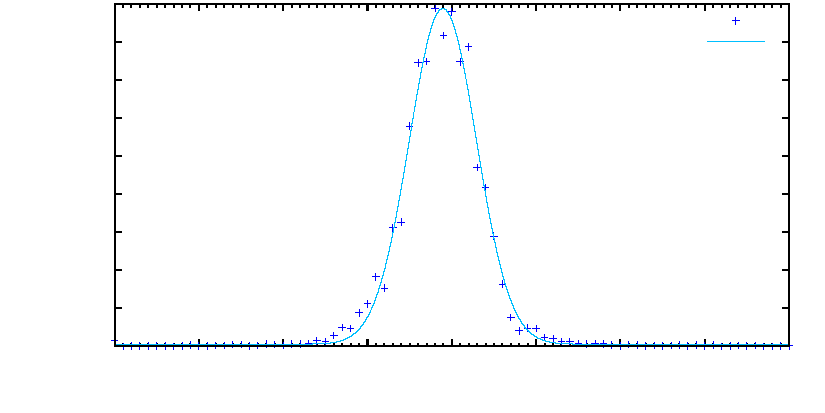
\includegraphics{linienscans_neues_schema_02_FES}}%
    \gplfronttext
  \end{picture}%
\endgroup

	}
	}}
	\caption[erster und zweiter Anregungsschritt, neues System, Schema (2)]{Linien
	der ersten beiden Übergänge des in Abb. \ref{fig:anregungsschema_neu_02}
	gezeigten Anregungsschemas.}
	\label{fig:linienscans_neues_schema_02}
\end{figure}
% \begin{figure}[hp]
%  	\centering
%  	\footnotesize
%  	\fbox{\parbox{\dimexpr \linewidth - 2\fboxrule - 2\fboxsep}{
%  	\subfloat[AI-Resonanzen zwischen $785,150\,$nm und $785,175\,$nm]{
% 		\label{subfig:linienscans_neues_schema_02_AI_01_mean}
% %		% GNUPLOT: LaTeX picture with Postscript
\begingroup
  \makeatletter
  \providecommand\color[2][]{%
    \GenericError{(gnuplot) \space\space\space\@spaces}{%
      Package color not loaded in conjunction with
      terminal option `colourtext'%
    }{See the gnuplot documentation for explanation.%
    }{Either use 'blacktext' in gnuplot or load the package
      color.sty in LaTeX.}%
    \renewcommand\color[2][]{}%
  }%
  \providecommand\includegraphics[2][]{%
    \GenericError{(gnuplot) \space\space\space\@spaces}{%
      Package graphicx or graphics not loaded%
    }{See the gnuplot documentation for explanation.%
    }{The gnuplot epslatex terminal needs graphicx.sty or graphics.sty.}%
    \renewcommand\includegraphics[2][]{}%
  }%
  \providecommand\rotatebox[2]{#2}%
  \@ifundefined{ifGPcolor}{%
    \newif\ifGPcolor
    \GPcolortrue
  }{}%
  \@ifundefined{ifGPblacktext}{%
    \newif\ifGPblacktext
    \GPblacktexttrue
  }{}%
  % define a \g@addto@macro without @ in the name:
  \let\gplgaddtomacro\g@addto@macro
  % define empty templates for all commands taking text:
  \gdef\gplbacktext{}%
  \gdef\gplfronttext{}%
  \makeatother
  \ifGPblacktext
    % no textcolor at all
    \def\colorrgb#1{}%
    \def\colorgray#1{}%
  \else
    % gray or color?
    \ifGPcolor
      \def\colorrgb#1{\color[rgb]{#1}}%
      \def\colorgray#1{\color[gray]{#1}}%
      \expandafter\def\csname LTw\endcsname{\color{white}}%
      \expandafter\def\csname LTb\endcsname{\color{black}}%
      \expandafter\def\csname LTa\endcsname{\color{black}}%
      \expandafter\def\csname LT0\endcsname{\color[rgb]{1,0,0}}%
      \expandafter\def\csname LT1\endcsname{\color[rgb]{0,1,0}}%
      \expandafter\def\csname LT2\endcsname{\color[rgb]{0,0,1}}%
      \expandafter\def\csname LT3\endcsname{\color[rgb]{1,0,1}}%
      \expandafter\def\csname LT4\endcsname{\color[rgb]{0,1,1}}%
      \expandafter\def\csname LT5\endcsname{\color[rgb]{1,1,0}}%
      \expandafter\def\csname LT6\endcsname{\color[rgb]{0,0,0}}%
      \expandafter\def\csname LT7\endcsname{\color[rgb]{1,0.3,0}}%
      \expandafter\def\csname LT8\endcsname{\color[rgb]{0.5,0.5,0.5}}%
    \else
      % gray
      \def\colorrgb#1{\color{black}}%
      \def\colorgray#1{\color[gray]{#1}}%
      \expandafter\def\csname LTw\endcsname{\color{white}}%
      \expandafter\def\csname LTb\endcsname{\color{black}}%
      \expandafter\def\csname LTa\endcsname{\color{black}}%
      \expandafter\def\csname LT0\endcsname{\color{black}}%
      \expandafter\def\csname LT1\endcsname{\color{black}}%
      \expandafter\def\csname LT2\endcsname{\color{black}}%
      \expandafter\def\csname LT3\endcsname{\color{black}}%
      \expandafter\def\csname LT4\endcsname{\color{black}}%
      \expandafter\def\csname LT5\endcsname{\color{black}}%
      \expandafter\def\csname LT6\endcsname{\color{black}}%
      \expandafter\def\csname LT7\endcsname{\color{black}}%
      \expandafter\def\csname LT8\endcsname{\color{black}}%
    \fi
  \fi
  \setlength{\unitlength}{0.0500bp}%
  \begin{picture}(7936.00,3968.00)%
    \gplgaddtomacro\gplbacktext{%
      \csname LTb\endcsname%
      \put(980,640){\makebox(0,0)[r]{\strut{} 0}}%
      \put(980,1297){\makebox(0,0)[r]{\strut{} 500}}%
      \put(980,1955){\makebox(0,0)[r]{\strut{} 1000}}%
      \put(980,2612){\makebox(0,0)[r]{\strut{} 1500}}%
      \put(980,3270){\makebox(0,0)[r]{\strut{} 2000}}%
      \put(980,3927){\makebox(0,0)[r]{\strut{} 2500}}%
      \put(1100,440){\makebox(0,0){\strut{} 381.816}}%
      \put(2025,440){\makebox(0,0){\strut{} 381.818}}%
      \put(2950,440){\makebox(0,0){\strut{} 381.82}}%
      \put(3875,440){\makebox(0,0){\strut{} 381.822}}%
      \put(4800,440){\makebox(0,0){\strut{} 381.824}}%
      \put(5725,440){\makebox(0,0){\strut{} 381.826}}%
      \put(6650,440){\makebox(0,0){\strut{} 381.828}}%
      \put(7575,440){\makebox(0,0){\strut{} 381.83}}%
      \put(160,2283){\rotatebox{-270}{\makebox(0,0){\strut{}Countrate [s$^{-1}$]}}}%
      \put(4337,140){\makebox(0,0){\strut{}Frequenz [THz]}}%
      \put(4338,2941){\makebox(0,0)[l]{\strut{}$F_{\text{sum}}=\sum\limits_{k=1}^2\frac{\left(\nicefrac{q_k\Gamma_k}{2}+\nu-\nu_k\right)^2}{(\nu-\nu_k)^2+\left(\nicefrac{\Gamma_k}{2}\right)^2}$}}%
      \put(4338,2382){\makebox(0,0)[l]{\strut{}$\Gamma_1 = (1.233\pm0.012)\,$GHz}}%
      \put(4338,2152){\makebox(0,0)[l]{\strut{}$\nu_1 = (381.818729\pm0.000006)\,$THz}}%
      \put(4338,1922){\makebox(0,0)[l]{\strut{}$q_1 = 46.11\pm0.16$}}%
      \put(4338,1692){\makebox(0,0)[l]{\strut{}$\Gamma_2 = (2.0\pm1.2)\,$GHz}}%
      \put(4338,1462){\makebox(0,0)[l]{\strut{}$\nu_2 = (381.82658\pm0.00041)\,$THz}}%
      \put(4338,1232){\makebox(0,0)[l]{\strut{}$q_2 = 8.1\pm1.7$}}%
    }%
    \gplgaddtomacro\gplfronttext{%
      \csname LTb\endcsname%
      \put(6672,3764){\makebox(0,0)[r]{\strut{}Messpunkte}}%
      \csname LTb\endcsname%
      \put(6672,3564){\makebox(0,0)[r]{\strut{}Fit}}%
    }%
    \gplbacktext
    \put(0,0){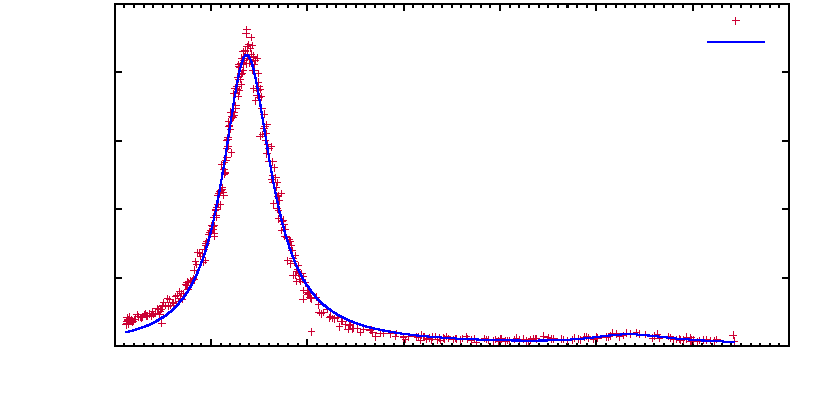
\includegraphics{linienscans_neues_schema_02_AI_01_mean}}%
    \gplfronttext
  \end{picture}%
\endgroup

% 	}\\
%  	\subfloat[AI-Resonanzen zwischen $782,46\,$nm und $782,50\,$nm]{
% 		\label{subfig:linienscans_neues_schema_02_AI_02_mean}
% 		% GNUPLOT: LaTeX picture with Postscript
\begingroup
  \makeatletter
  \providecommand\color[2][]{%
    \GenericError{(gnuplot) \space\space\space\@spaces}{%
      Package color not loaded in conjunction with
      terminal option `colourtext'%
    }{See the gnuplot documentation for explanation.%
    }{Either use 'blacktext' in gnuplot or load the package
      color.sty in LaTeX.}%
    \renewcommand\color[2][]{}%
  }%
  \providecommand\includegraphics[2][]{%
    \GenericError{(gnuplot) \space\space\space\@spaces}{%
      Package graphicx or graphics not loaded%
    }{See the gnuplot documentation for explanation.%
    }{The gnuplot epslatex terminal needs graphicx.sty or graphics.sty.}%
    \renewcommand\includegraphics[2][]{}%
  }%
  \providecommand\rotatebox[2]{#2}%
  \@ifundefined{ifGPcolor}{%
    \newif\ifGPcolor
    \GPcolortrue
  }{}%
  \@ifundefined{ifGPblacktext}{%
    \newif\ifGPblacktext
    \GPblacktexttrue
  }{}%
  % define a \g@addto@macro without @ in the name:
  \let\gplgaddtomacro\g@addto@macro
  % define empty templates for all commands taking text:
  \gdef\gplbacktext{}%
  \gdef\gplfronttext{}%
  \makeatother
  \ifGPblacktext
    % no textcolor at all
    \def\colorrgb#1{}%
    \def\colorgray#1{}%
  \else
    % gray or color?
    \ifGPcolor
      \def\colorrgb#1{\color[rgb]{#1}}%
      \def\colorgray#1{\color[gray]{#1}}%
      \expandafter\def\csname LTw\endcsname{\color{white}}%
      \expandafter\def\csname LTb\endcsname{\color{black}}%
      \expandafter\def\csname LTa\endcsname{\color{black}}%
      \expandafter\def\csname LT0\endcsname{\color[rgb]{1,0,0}}%
      \expandafter\def\csname LT1\endcsname{\color[rgb]{0,1,0}}%
      \expandafter\def\csname LT2\endcsname{\color[rgb]{0,0,1}}%
      \expandafter\def\csname LT3\endcsname{\color[rgb]{1,0,1}}%
      \expandafter\def\csname LT4\endcsname{\color[rgb]{0,1,1}}%
      \expandafter\def\csname LT5\endcsname{\color[rgb]{1,1,0}}%
      \expandafter\def\csname LT6\endcsname{\color[rgb]{0,0,0}}%
      \expandafter\def\csname LT7\endcsname{\color[rgb]{1,0.3,0}}%
      \expandafter\def\csname LT8\endcsname{\color[rgb]{0.5,0.5,0.5}}%
    \else
      % gray
      \def\colorrgb#1{\color{black}}%
      \def\colorgray#1{\color[gray]{#1}}%
      \expandafter\def\csname LTw\endcsname{\color{white}}%
      \expandafter\def\csname LTb\endcsname{\color{black}}%
      \expandafter\def\csname LTa\endcsname{\color{black}}%
      \expandafter\def\csname LT0\endcsname{\color{black}}%
      \expandafter\def\csname LT1\endcsname{\color{black}}%
      \expandafter\def\csname LT2\endcsname{\color{black}}%
      \expandafter\def\csname LT3\endcsname{\color{black}}%
      \expandafter\def\csname LT4\endcsname{\color{black}}%
      \expandafter\def\csname LT5\endcsname{\color{black}}%
      \expandafter\def\csname LT6\endcsname{\color{black}}%
      \expandafter\def\csname LT7\endcsname{\color{black}}%
      \expandafter\def\csname LT8\endcsname{\color{black}}%
    \fi
  \fi
  \setlength{\unitlength}{0.0500bp}%
  \begin{picture}(7936.00,3968.00)%
    \gplgaddtomacro\gplbacktext{%
      \csname LTb\endcsname%
      \put(980,640){\makebox(0,0)[r]{\strut{} 0}}%
      \put(980,969){\makebox(0,0)[r]{\strut{} 100}}%
      \put(980,1297){\makebox(0,0)[r]{\strut{} 200}}%
      \put(980,1626){\makebox(0,0)[r]{\strut{} 300}}%
      \put(980,1955){\makebox(0,0)[r]{\strut{} 400}}%
      \put(980,2283){\makebox(0,0)[r]{\strut{} 500}}%
      \put(980,2612){\makebox(0,0)[r]{\strut{} 600}}%
      \put(980,2941){\makebox(0,0)[r]{\strut{} 700}}%
      \put(980,3270){\makebox(0,0)[r]{\strut{} 800}}%
      \put(980,3598){\makebox(0,0)[r]{\strut{} 900}}%
      \put(980,3927){\makebox(0,0)[r]{\strut{} 1000}}%
      \put(1100,440){\makebox(0,0){\strut{} 383.115}}%
      \put(2025,440){\makebox(0,0){\strut{} 383.12}}%
      \put(2950,440){\makebox(0,0){\strut{} 383.125}}%
      \put(3875,440){\makebox(0,0){\strut{} 383.13}}%
      \put(4800,440){\makebox(0,0){\strut{} 383.135}}%
      \put(5725,440){\makebox(0,0){\strut{} 383.14}}%
      \put(6650,440){\makebox(0,0){\strut{} 383.145}}%
      \put(7575,440){\makebox(0,0){\strut{} 383.15}}%
      \put(160,2283){\rotatebox{-270}{\makebox(0,0){\strut{}Countrate [s$^{-1}$]}}}%
      \put(4337,140){\makebox(0,0){\strut{}Relativfrequenz [MHz]}}%
    }%
    \gplgaddtomacro\gplfronttext{%
      \csname LTb\endcsname%
      \put(6672,3764){\makebox(0,0)[r]{\strut{}Messpunkte}}%
      \csname LTb\endcsname%
      \put(6672,3564){\makebox(0,0)[r]{\strut{}Fit}}%
    }%
    \gplbacktext
    \put(0,0){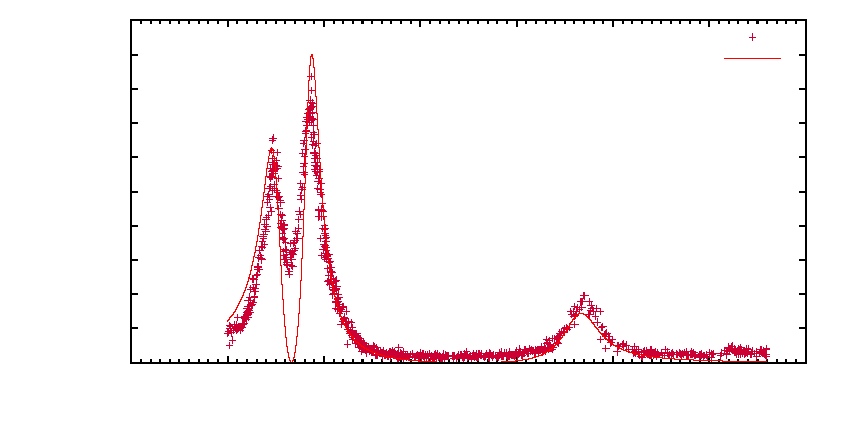
\includegraphics{linienscans_neues_schema_02_AI_02_mean}}%
    \gplfronttext
  \end{picture}%
\endgroup

% 	}
% 	}}
% 	\caption[AIs, neues System, Schema (2)]{AIs für das Schema aus Abb.
% \ref{fig:anregungsschema_neu_02}.}
% \label{fig:linienscans_neues_schema_02_AIs}
% \end{figure}
% TODO: !!!AI-Fits
Wie erwartet sind in diesem AI-Spektrum einige vergleichsweise schmale AIs zu
finden. Um weitere Aussagen über dieses Schema machen zu können, sind in der
Zukunft weitere Messungen vorgesehen.

\subsection{Weitere geplante spektroskopische
Messungen}\label{subsec:geplante_messungen}
In diesem Abschnitt sollen kurz alle weiteren in naher Zukunft geplanten
spektroskopische Messungen aufgelistet werden, deren Ergebnisse in einer in
Arbeit befindlichen Doktorarbeit \cite{hakimi:2012:dissertation} in der
Arbeitsgruppe ausgeführt werden sollen:
\begin{setlength}{\leftmargini}{0cm}
	\begin{description}
	\item[1)]Zunächst soll das alten Schema auf dem neuen System simuliert werden. Dazu
		werden die beiden \textit{Toptica}-Laser als zweiter und dritter Schritt
		parallel mit dem blauen Laser aus dem alten System verwendet. Bei schnellem
		Wechsel auf die Laser des alten Systems z.B. über Verwendung von Klapp- oder
		Magnetspiegeln lässt sich so ein direkter Performacevergleich beider Systeme
		aufstellen.
	\item[2)]Die Untersuchung des neu gefundenen intensiven, zweiten
		Anregungsschritts aus Abb.
		\ref{fig:linienscans_neues_schema_01_fake_AI_krass_mean} soll fortgeführt
		werden. Aus dem FES des zweiten neuen Schemas
		(Abb. \ref{fig:anregungsschema_neu_02}) soll dieser zweite Schritt getestet
		werden. Hierzu sollen auch nochmals breitbandige AI-Scans unter Verwendung
		gepulster Laser durchgeführt werden.
	\item[3)]Eine weitere Idee ist es, alle mit dem $405\,$nm-Diodenlaser erreichbaren
		Niveaus mit dem frequenzverdoppelten Licht des \textit{TA-Pro} ($389\,$nm) zu
		besetzen. Der Vorteil hierbei ist, dass im Gegensatz zu dem thermisch angeregten
		Zustand von dem weitaus stärker besetzten GZ ausgegangen wird, wobei eine
		Steigerung von Effizienz und Selektivität zu erwarten ist.
	\end{description}
\end{setlength} 


% \section{Zählratenfluktuation}\label{sec:countraten_fluktuation}
% Im Rahmen der Spektroskopiemessungen wurden auch Zahlratenfluktuationen beider
% Systeme aufgenommen. Dazu wurde für das alte bzw. neue System das
% Anregungsschema aus Abb. \ref{fig:anregungsschema_alt} bzw.
% \ref{fig:anregungsschema_neu_02} verwendet. Die Zählraten wurden bei
% Integrationszeiten von $0,1\,$s, $1\,$s, $2\,$s und $4\,$s aufgenommen.
% In Tab. \ref{tab:countraten_fluktuationen} und Abb.
% \ref{fig:countraten_fluktuationen} sind die Ergebnisse der Statistik dieser
% Messung dargestellt.
% \begin{table}[h]
% 	%Summe der Breiten muss 0.91 mal \textwidth sein.
% 	\begin{tabular}{cc|cccc}
% 		\toprule
% 		\multicolumn{1}{C{0.07\textwidth}}{T [s]} &
% 		\multicolumn{1}{C{0.07\textwidth}}{} &
% 		\multicolumn{1}{C{0.16\textwidth}}{$n$} &
% 		\multicolumn{1}{C{0.16\textwidth}}{$\mu$ [$\nicefrac{1}{T}$]} &
% 		\multicolumn{1}{C{0.16\textwidth}}{$\sigma$ [$\nicefrac{1}{T}$]} &
% 		\multicolumn{1}{C{0.16\textwidth}}{$\nicefrac{\sigma}{\mu}$ [\%]}\\
% 		\midrule[1px]
% 		\hline
% 		\multirow{2}{*}{0,1} & alt & $215$ & $4447$ & $437$ & $9,8$ \\
% 		& neu & $95$ & $123$ & $19$ & $16$ \\
% 		\hline
% 		\multirow{2}{*}{1} & alt & $101$ & $41387$ & $2019$ & $4,9$ \\
% 		& neu & $46$ & $1265$ & $100$ & $7,9$ \\
% 		\hline
% 		\multirow{2}{*}{2} & alt & $74$ & $90773$ & $4792$ & $5,3$ \\
% 		& neu & $46$ & $2577$ & $137$ & $5,3$ \\
% 		\hline
% 		\multirow{2}{*}{4} & alt & $74$ & $222052$ & $8757$ & $3,9$ \\
% 		& neu & $46$ & $5085$ & $256$ & $5,0$ \\
% 		\bottomrule[1px]
% 	\end{tabular}
% 	\caption[Zählratenfluktuationen]{Ergebnisse der
% 	Zählratenfluktuationsmessung beider Systeme. Berechnet wurden Mittelwert $\mu$
% 	der Zählraten, Standardabweichung $\sigma$ und prozentuale Fluktuation
% 	$\nicefrac{\sigma}{\mu}$ bei verschiedenen Integrationszeiten $T$, wobei $n$ Messwerte in die Berechnung eingeflossen sind.}
% 	\label{tab:countraten_fluktuationen}
% \end{table}
% \begin{figure}[h]
%  	\centering
%  	\footnotesize
% 	% GNUPLOT: LaTeX picture with Postscript
\begingroup
  \makeatletter
  \providecommand\color[2][]{%
    \GenericError{(gnuplot) \space\space\space\@spaces}{%
      Package color not loaded in conjunction with
      terminal option `colourtext'%
    }{See the gnuplot documentation for explanation.%
    }{Either use 'blacktext' in gnuplot or load the package
      color.sty in LaTeX.}%
    \renewcommand\color[2][]{}%
  }%
  \providecommand\includegraphics[2][]{%
    \GenericError{(gnuplot) \space\space\space\@spaces}{%
      Package graphicx or graphics not loaded%
    }{See the gnuplot documentation for explanation.%
    }{The gnuplot epslatex terminal needs graphicx.sty or graphics.sty.}%
    \renewcommand\includegraphics[2][]{}%
  }%
  \providecommand\rotatebox[2]{#2}%
  \@ifundefined{ifGPcolor}{%
    \newif\ifGPcolor
    \GPcolortrue
  }{}%
  \@ifundefined{ifGPblacktext}{%
    \newif\ifGPblacktext
    \GPblacktexttrue
  }{}%
  % define a \g@addto@macro without @ in the name:
  \let\gplgaddtomacro\g@addto@macro
  % define empty templates for all commands taking text:
  \gdef\gplbacktext{}%
  \gdef\gplfronttext{}%
  \makeatother
  \ifGPblacktext
    % no textcolor at all
    \def\colorrgb#1{}%
    \def\colorgray#1{}%
  \else
    % gray or color?
    \ifGPcolor
      \def\colorrgb#1{\color[rgb]{#1}}%
      \def\colorgray#1{\color[gray]{#1}}%
      \expandafter\def\csname LTw\endcsname{\color{white}}%
      \expandafter\def\csname LTb\endcsname{\color{black}}%
      \expandafter\def\csname LTa\endcsname{\color{black}}%
      \expandafter\def\csname LT0\endcsname{\color[rgb]{1,0,0}}%
      \expandafter\def\csname LT1\endcsname{\color[rgb]{0,1,0}}%
      \expandafter\def\csname LT2\endcsname{\color[rgb]{0,0,1}}%
      \expandafter\def\csname LT3\endcsname{\color[rgb]{1,0,1}}%
      \expandafter\def\csname LT4\endcsname{\color[rgb]{0,1,1}}%
      \expandafter\def\csname LT5\endcsname{\color[rgb]{1,1,0}}%
      \expandafter\def\csname LT6\endcsname{\color[rgb]{0,0,0}}%
      \expandafter\def\csname LT7\endcsname{\color[rgb]{1,0.3,0}}%
      \expandafter\def\csname LT8\endcsname{\color[rgb]{0.5,0.5,0.5}}%
    \else
      % gray
      \def\colorrgb#1{\color{black}}%
      \def\colorgray#1{\color[gray]{#1}}%
      \expandafter\def\csname LTw\endcsname{\color{white}}%
      \expandafter\def\csname LTb\endcsname{\color{black}}%
      \expandafter\def\csname LTa\endcsname{\color{black}}%
      \expandafter\def\csname LT0\endcsname{\color{black}}%
      \expandafter\def\csname LT1\endcsname{\color{black}}%
      \expandafter\def\csname LT2\endcsname{\color{black}}%
      \expandafter\def\csname LT3\endcsname{\color{black}}%
      \expandafter\def\csname LT4\endcsname{\color{black}}%
      \expandafter\def\csname LT5\endcsname{\color{black}}%
      \expandafter\def\csname LT6\endcsname{\color{black}}%
      \expandafter\def\csname LT7\endcsname{\color{black}}%
      \expandafter\def\csname LT8\endcsname{\color{black}}%
    \fi
  \fi
  \setlength{\unitlength}{0.0500bp}%
  \begin{picture}(7200.00,5040.00)%
    \gplgaddtomacro\gplbacktext{%
      \csname LTb\endcsname%
      \put(740,640){\makebox(0,0)[r]{\strut{} 2}}%
      \put(740,1234){\makebox(0,0)[r]{\strut{} 4}}%
      \put(740,1828){\makebox(0,0)[r]{\strut{} 6}}%
      \put(740,2422){\makebox(0,0)[r]{\strut{} 8}}%
      \put(740,3017){\makebox(0,0)[r]{\strut{} 10}}%
      \put(740,3611){\makebox(0,0)[r]{\strut{} 12}}%
      \put(740,4205){\makebox(0,0)[r]{\strut{} 14}}%
      \put(740,4799){\makebox(0,0)[r]{\strut{} 16}}%
      \put(860,440){\makebox(0,0){\strut{} 0}}%
      \put(1607,440){\makebox(0,0){\strut{} 0.5}}%
      \put(2355,440){\makebox(0,0){\strut{} 1}}%
      \put(3102,440){\makebox(0,0){\strut{} 1.5}}%
      \put(3850,440){\makebox(0,0){\strut{} 2}}%
      \put(4597,440){\makebox(0,0){\strut{} 2.5}}%
      \put(5344,440){\makebox(0,0){\strut{} 3}}%
      \put(6092,440){\makebox(0,0){\strut{} 3.5}}%
      \put(6839,440){\makebox(0,0){\strut{} 4}}%
      \put(160,2719){\rotatebox{-270}{\makebox(0,0){\strut{}Fluktuation [\%]}}}%
      \put(3849,140){\makebox(0,0){\strut{}Integrationszeit [s]}}%
    }%
    \gplgaddtomacro\gplfronttext{%
      \csname LTb\endcsname%
      \put(5936,4636){\makebox(0,0)[r]{\strut{}altes System}}%
      \csname LTb\endcsname%
      \put(5936,4436){\makebox(0,0)[r]{\strut{}neues System}}%
    }%
    \gplbacktext
    \put(0,0){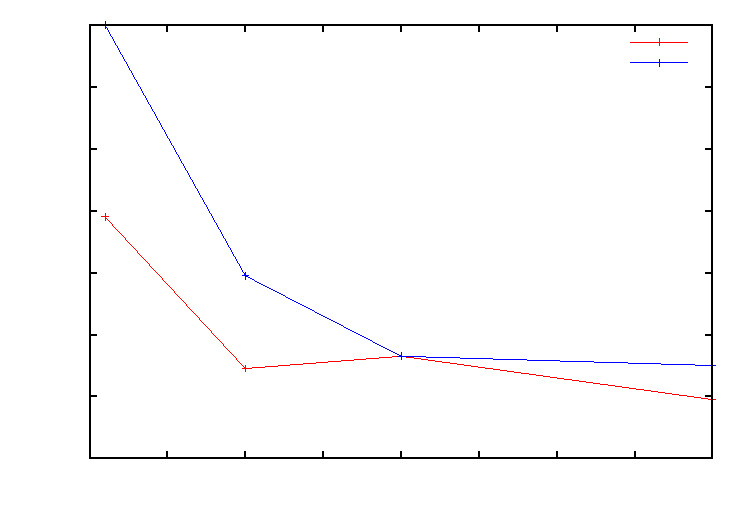
\includegraphics{countraten_fluktuationen}}%
    \gplfronttext
  \end{picture}%
\endgroup

% 	\caption[Zählratenfluktuationen]{Geplottet sind die
% 	prozentualen Zählratenfluktuationen gegen die Integrationszeit.}
% 	\label{fig:countraten_fluktuationen}
% \end{figure}
% Das neue System weist mit dem momentanen Aufbau eine höhere Zählratenfluktuation
% auf, was alleine auf das Laserfrequenzverhalten bezogen einen Widerspruch
% darstellt. Es wird vermutet, dass die erhöhte Fluktuation aus dem wesentlich
% längen Strahltransport resultiert, wobei räumliche Fluktuationen eine
% entscheidende Rolle spielen.
